\documentclass{article}
\input{../../../LaTex/preamble/preamble_article.tex}

\begin{comment}
    重复语句
    \subsubsection{}
    \includegraphics[width=50em,keepaspectratio]{}

    \begin{itemize}
        \item 错选:\quad
        \item 正解:\quad
        \item 总结:\quad
        \item 扩展:\quad
    \end{itemize}

\end{comment}


\title{高中物理精题集}
\author{马祥芸}

\begin{document}
\maketitle
\tableofcontents
\newpage

\section{高一}

\subsection{2022-2023年度(下)重庆八中高一期末}

\subsubsection{I-7:荷质比问题}
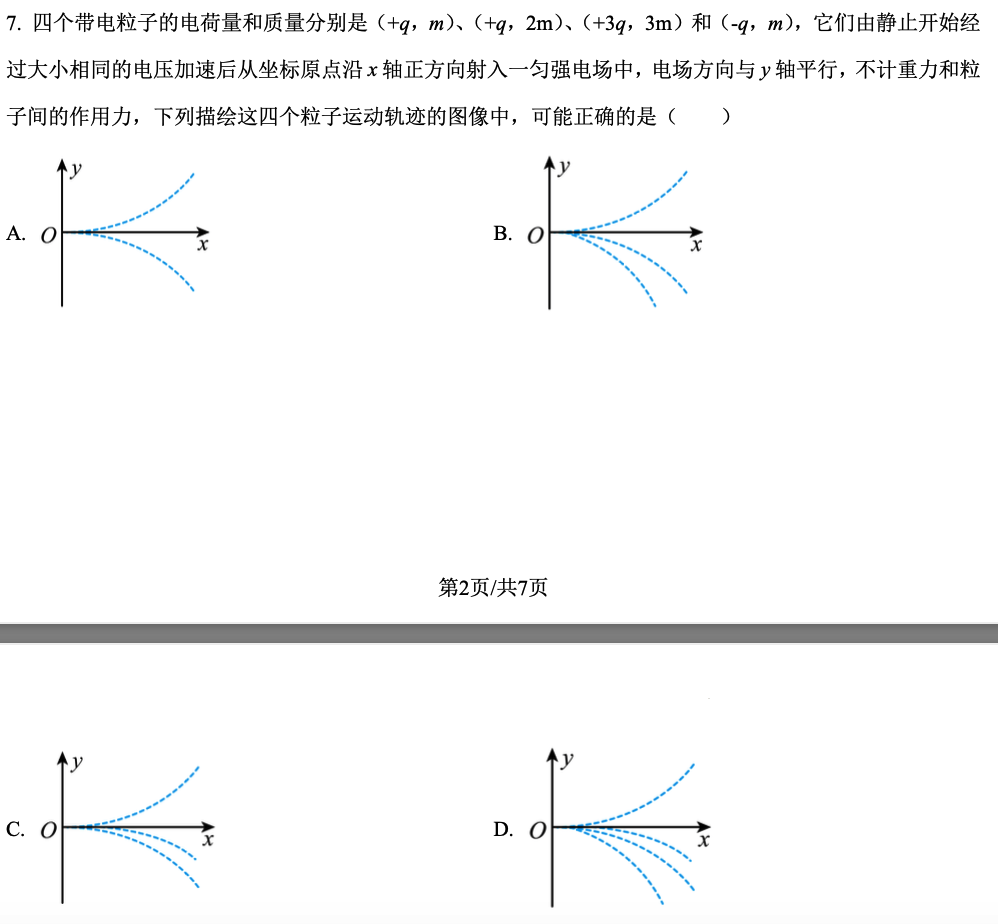
\includegraphics[width=0.95\textwidth,keepaspectratio]{./pictures/1.1-1.png}

\begin{itemize}
    \item 正解:\quad $A$
    \item 总结:最终要给出\textbf{轨迹方程,即$ y = f(x) $},同时注意\textbf{电荷的正负性}决定着轨迹函数所在的区间
    \item 扩展:荷质比相关题目,粒子回旋加速期、粒子速度筛选器等
\end{itemize}

\vspace{2em}

\subsubsection{II-9:不同类型的碰撞}
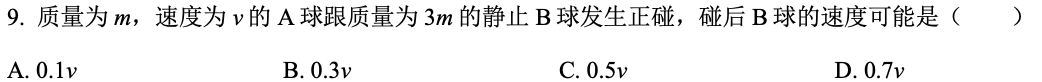
\includegraphics[width=0.95\textwidth,keepaspectratio]{./pictures/1.1-2.png}

\begin{itemize}
    \item 正解:\quad $BC$
    \item 总结:\quad 容易用不等式解法去求得$3m$物块的最大速度,但是无法计算最小速度。事实上$3m$物体碰
          后的\textbf{速度区间取决于碰撞过程中的动能损失程度}。
          \begin{itemize}
              \item \textbf{弹性碰撞(完全弹性碰撞)},系统机械能损失\textbf{最小},获得被碰物体\textbf{最大速度}
              \item \textbf{非弹性碰撞},系统机能损失,特点是碰后两物块\textbf{分离}
              \item \textbf{完全非弹性碰撞},碰撞后物体"粘连"  $ \lra mv_{0} = (m+3m)v^{'} $在一起,系统动能损失\textbf{最大},被碰物体获得\textbf{最小速度}。
          \end{itemize}
\end{itemize}

\vspace{2em}

\subsubsection{II-10:匀强电场下的斜射}
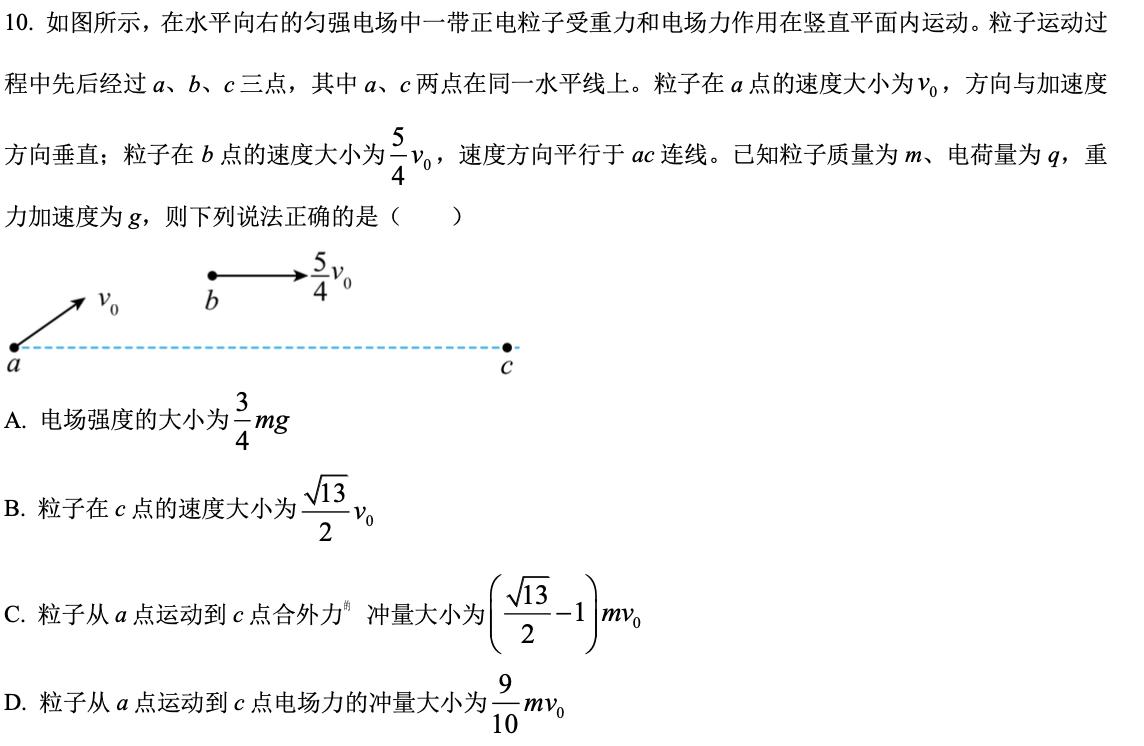
\includegraphics[width=0.95\textwidth,keepaspectratio]{./pictures/1.1-3.png}

\begin{itemize}
    \item 正解:\quad $BD$
    \item 总结:\quad
          \begin{itemize}
              \item 选项A \\
                    重点在于粒子在$a$点时的速度方向与加速度方向垂直。因此 \quad $b$点的速度在初速度方向的投影 \quad 与 \quad 初速度的大小一致。由此可以求得初始速度方向与水平方向的夹角$\theta$。再通过
                    相同时间内($a \rightarrow b$),重力冲量与电场力冲量下对两个方向的动量改变量,获得的两个方程消去时间$\triangle t$,得到$Eq$与$mg$的数量关系(选项$A$量纲错误)。
                    $$
                        \begin{cases}
                            mg \vdot \triangle t = m v_{0} \vdot \sin{\theta} \\
                            Eq \vdot \triangle t = \frac{5}{4} m v_{0} - m v_{0} \vdot \cos{\theta}
                        \end{cases}
                    $$

              \item 选项B \\
                    在同一水平面上,$a \rightarrow c$的时间为$a \rightarrow b$的时间的两倍(竖直运动的对称性).

                    \begin{align*}
                        mg \vdot t                     & = 2 m v_{0} \sin{\theta} \lra t = \frac{6 v_{0}}{5 g} \\
                        m v_{x} - m v_{0} \cos{\theta} & = Eq \vdot t \quad (Eq = \frac{3}{4} mg)
                    \end{align*}
                    计算合速度可以先使用水平方向上的冲量定理计算出水平方向上的速度。或者直接用动能定理(重力势能不变),计算出$a \rightarrow c$的水平距离,进而得到电场力做功。
          \end{itemize}
\end{itemize}

\vspace{2em}

\subsubsection{III-1:实验中的Q/U-t图像}
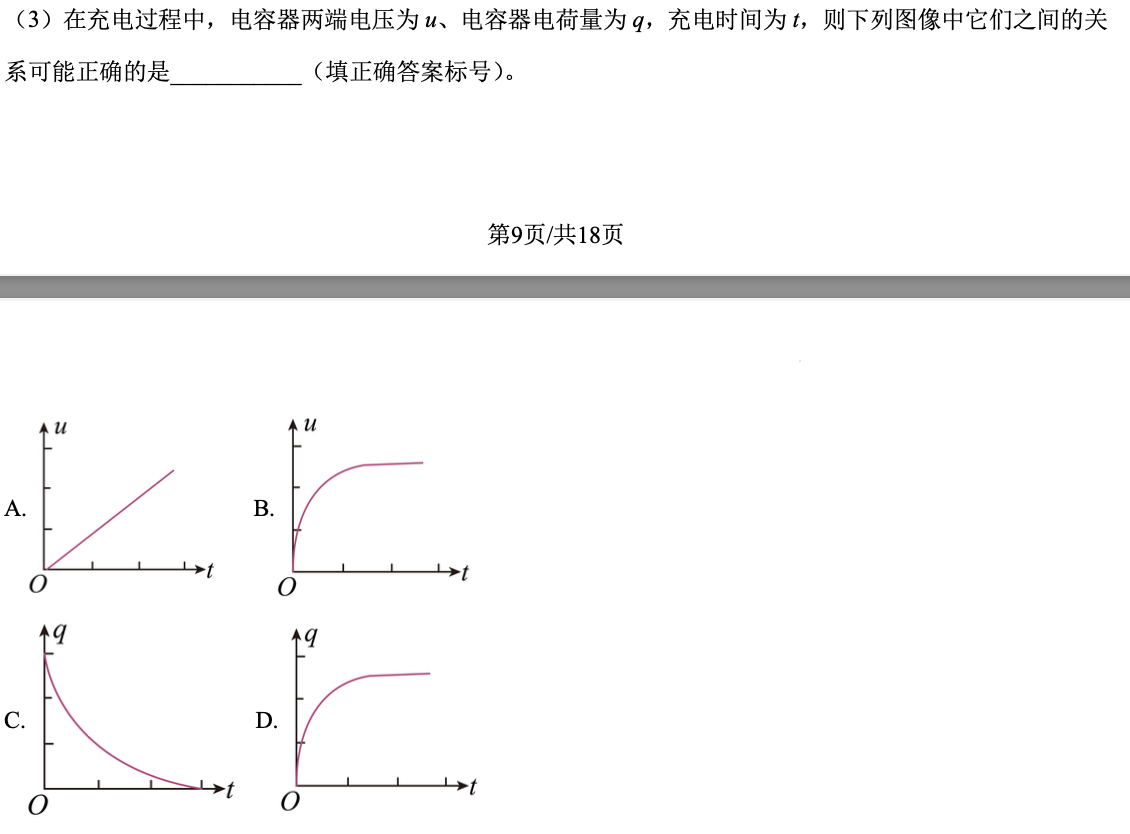
\includegraphics[width=0.95\textwidth,keepaspectratio]{./pictures/1.1-4.png}

\begin{itemize}
    \item 正解:\quad $BD$
    \item 总结:\quad 电容器的电压并非在一瞬间就获得,同样是电荷累计的结果
\end{itemize}

\vspace{2em}

\subsection{2022-2023育才中学期末模拟题(八)}

\subsubsection{I-4:关联体旋转运动分析}
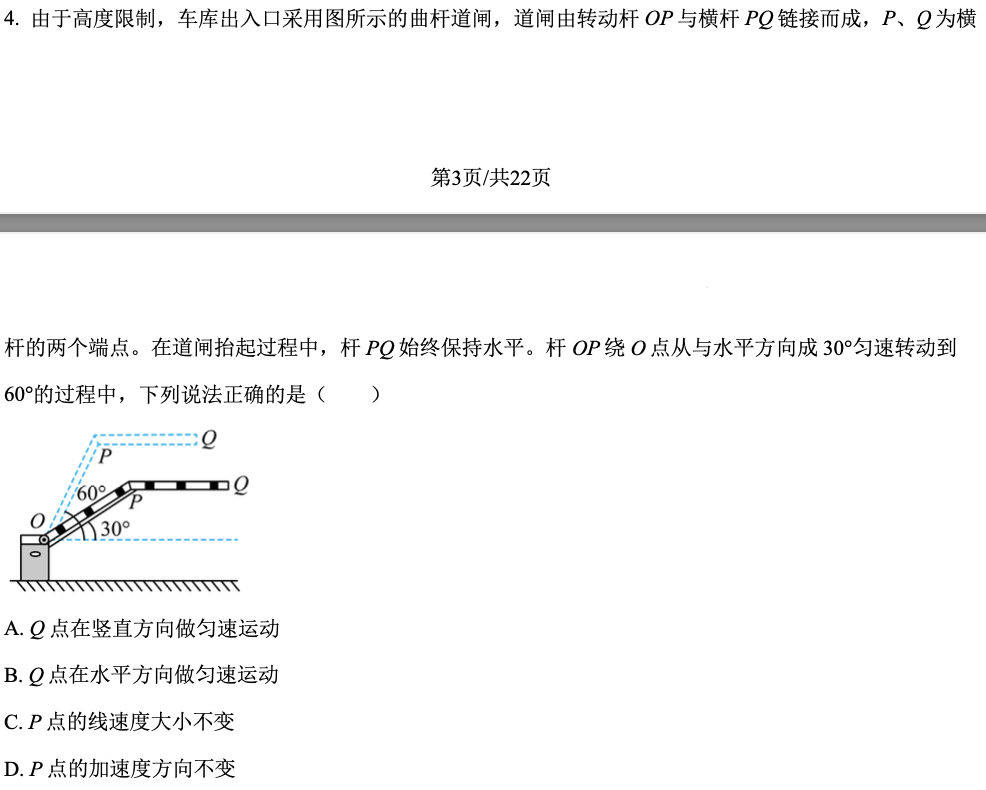
\includegraphics[width=0.95\textwidth,keepaspectratio]{./pictures/1.2-1.png}

\begin{itemize}
    \item 正解:\quad $C$
    \item 总结:\quad 选出正确答案并不难,本质是$\omega_{//}$
    \item 扩展:\quad 进一步思考本题,$P$点的运动为匀速圆周运动,因此其坐标$(x,y)$是可以被表示的.
          $$
              P_(x,y) = (\cos{(\omega t + \phi_{0})} , \sin{(\omega t + \phi_{0})})
          $$
          同时$Q$点的坐标也是可以被表示的,存在\textbf{几何约束},$P$到$Q$的距离为固定值线段$\overline{PQ} = L$,显然$Q$也是做匀速圆周运动
          圆心为距离圆心$O$右侧$L$处,且角速度小于$P$点.
\end{itemize}

\vspace{2em}

\subsubsection{I-7:P-t图问题}
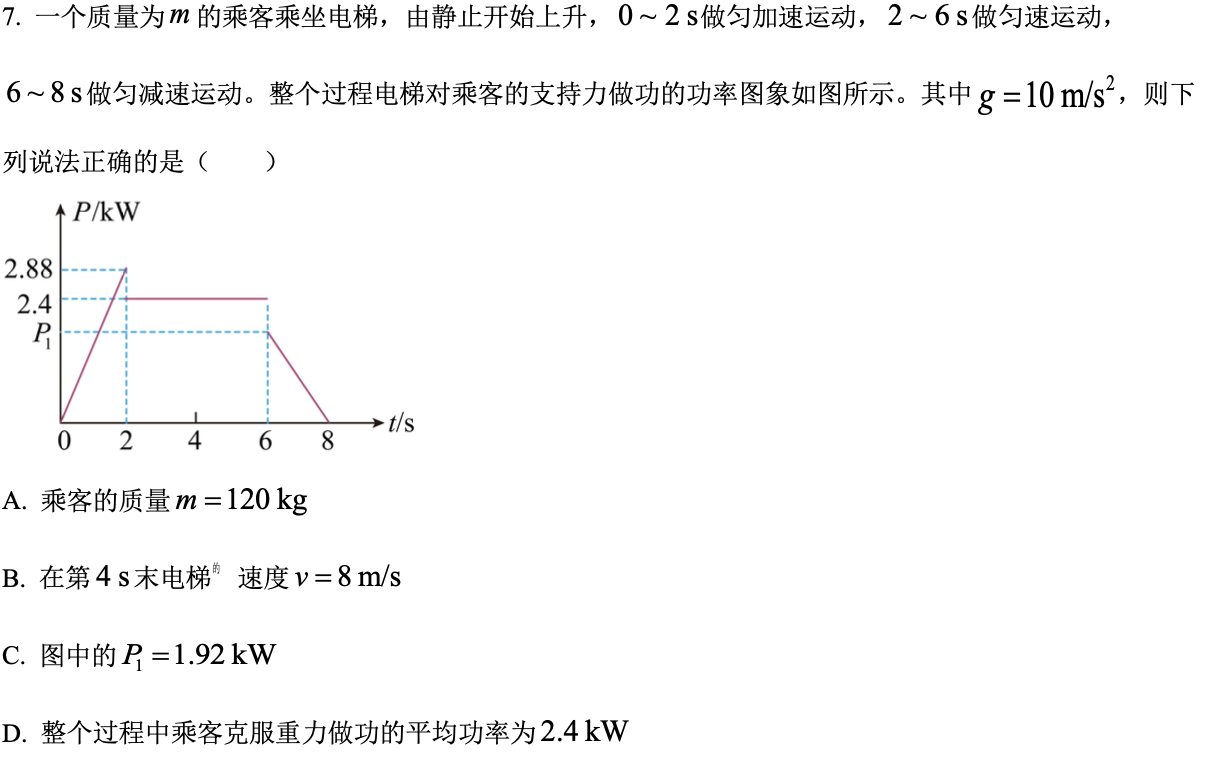
\includegraphics[width=0.95\textwidth,keepaspectratio]{./pictures/1.2-2.png}

\begin{itemize}
    \item 正解:\quad $C$
    \item 总结:\quad 此题分为三个阶段,同时存在一个重要的速度节点,即$t = 2s$时的速度.所列方程众多,因此理清阶段,以及要求的目标量.
          $$
              \begin{cases}
                  P_{1} = N \vdot a \vdot t = 2880 w \\
                  P_{2} = mg \vdot a \vdot t  = 2400 w
              \end{cases}
          $$
          选项$D$,可以有两种思路;第一种:计算出位移,得到重力势能做功.第二种$P-t$图所围成的面积为支持力做功的平均功率,在此过程中无
          其他力做功且初末动能均为0,因此支持力做功的平均功率等于克服重力做功的平均功率.
          $$ W = 1920j + 2880j + 9600 j \qquad t_{total} = 8s \qquad \overline{P} = \frac{W}{t_{total}} = 1.8kw $$

    \item 扩展:
          \begin{align}
              P & = N \vdot v \qquad v = v_{0} + a t \qquad v_{0} = 0 \qquad a = \frac{N-mg}{m} \\
              P & = \frac{N(N-mg)}{m} t \qquad  k = \frac{N(N-mg)}{m}
          \end{align}
\end{itemize}

\vspace{2em}

\subsubsection{II-8:水平内的碰撞+环形追及问题}
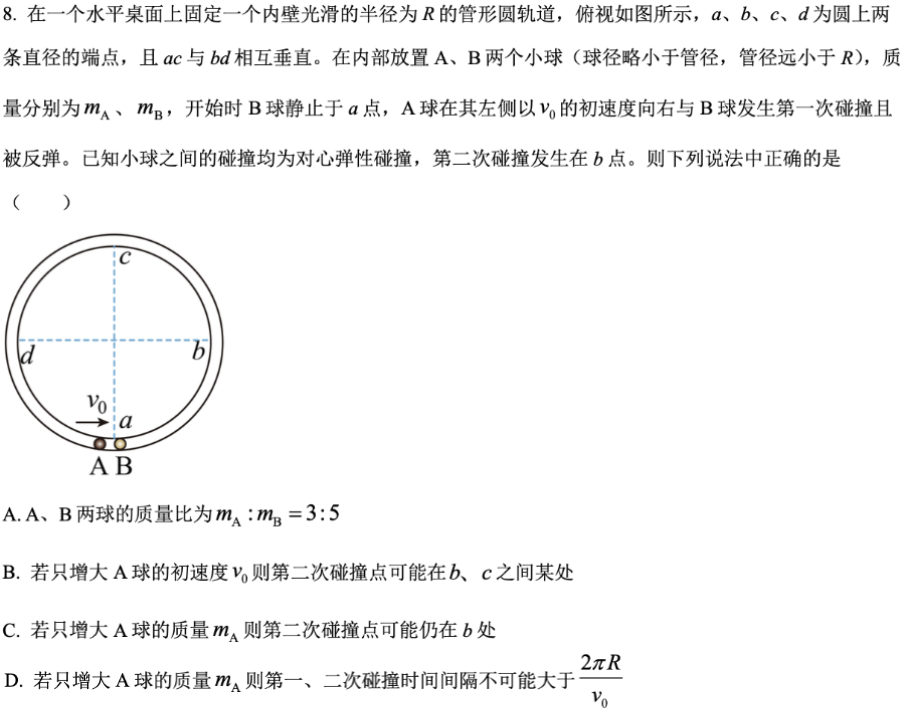
\includegraphics[width=0.95\textwidth,keepaspectratio]{./pictures/1.2-3.png}

\begin{itemize}
    \item 正解:\quad $CD$
    \item 总结:\quad 此物理情景发生在水平桌面上,所以不用考虑重力.所以本质是一个追及问题。同时第二次碰撞满足三个方程,第一个方程控制碰撞约束,第二、三个方程控制具体
          碰撞点
          $$
              \begin{cases}
                  v_{A} t + v_{B} t = 2 \pi R \\
                  v_{B} t  = \frac{\pi}{2}    \\
                  v_{A} t = \frac{3\pi}{2}
              \end{cases}
          $$
          选项$B$,通过前面的计算碰撞发生的时间为$t = \frac{2\pi R}{v_{0}}$ 仅仅与$v_{0}$有关,但碰后的速度也发生了变化,因此我们需要设出
          碰撞时的角度(这里取与水平线上为$\alpha$),计算出该角度的函数表达式(关于初速度质量等)
          $$
              \begin{cases}
                  v_{A} t & = (\frac{3\pi}{2} - \alpha) R           \\
                  v_{B} t & = (\frac{\pi}{2} + \alpha) R            \\
                  v_{A}   & = \frac{m_{B} - m{A}}{m_{A}+m{B}} v_{0} \\
                  v_{B}   & = \frac{2 m{A}}{m_{A}+m{B}} v_{0}
              \end{cases}
          $$

          $$
              \alpha = \frac{7 \pi}{2} \vdot \frac{m_{A} - m_{B}}{m_{A} + m_{B}}
          $$
          其碰撞点与初速度无关所以$B$错,与质量相关,当碰撞点在$b$时存在球$A$反向碰撞(题目初始情况)与球$A$同向被套圈碰撞,所以$C$对,满足$m_{A} : m_{B} = 5 : 3$
\end{itemize}

\vspace{2em}

\subsubsection{II-9:外轨道圆周运动问题}

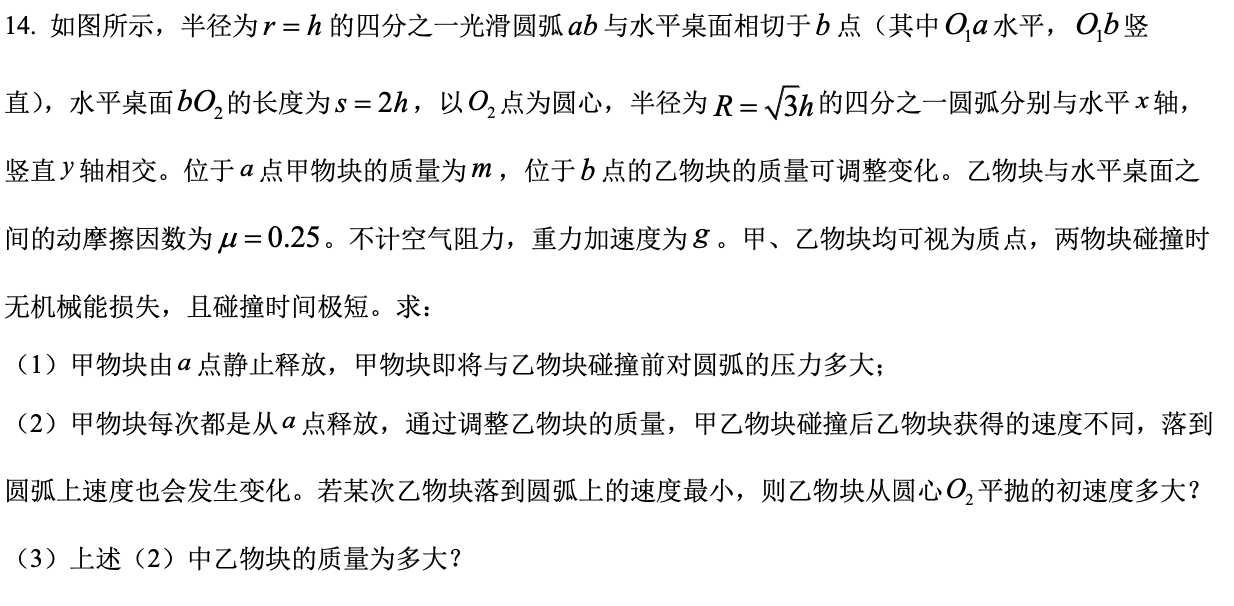
\includegraphics[width=0.95\textwidth,keepaspectratio]{./pictures/1.2-7.png}

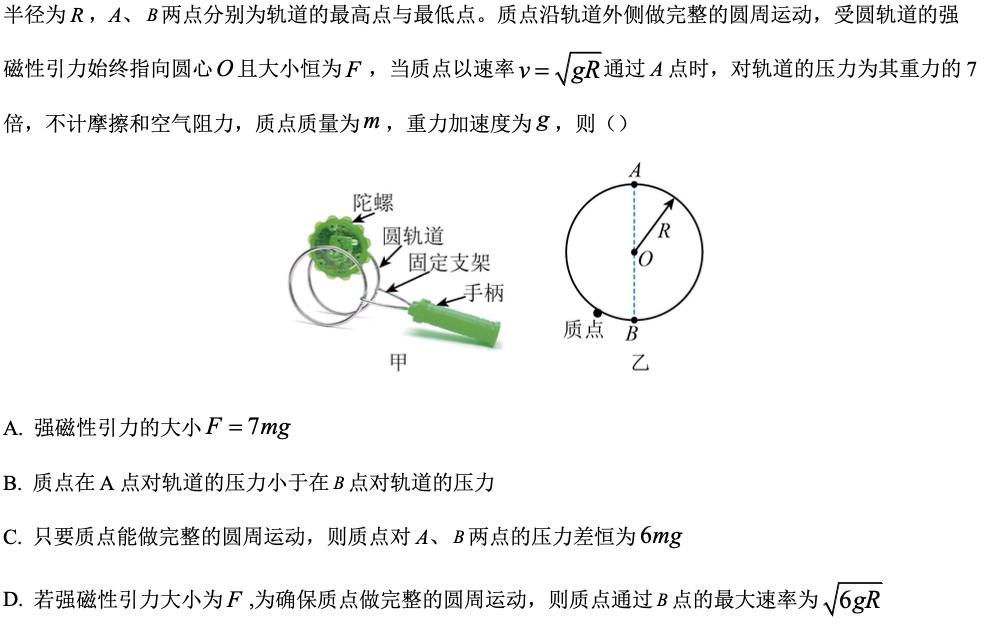
\includegraphics[width=0.95\textwidth,keepaspectratio]{./pictures/1.2-8.png}



\vspace{2em}

\subsubsection{III-12:动量守恒实验-圆弧约束}
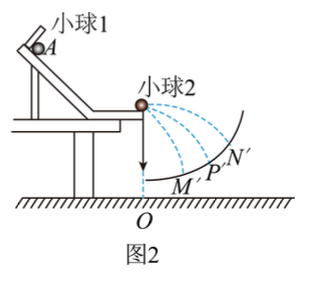
\includegraphics[width=0.95\textwidth,keepaspectratio]{./pictures/1.2-4.png}

\begin{itemize}
    \item 总结:夹角$\alpha$为位移偏转角.这类题目已知位移偏转角同时还有几何约束那么易得
          $$
              \begin{cases}
                  x = R \cos{\alpha} = v_{x} t             \\
                  y = R \sin{\alpha} = \frac{1}{2} g t^{2} \\
              \end{cases}
          $$

          $$
              \lra v_{x} = \sqrt{\frac{gR}{2}} \vdot \sqrt{\frac{\cos^{2}{\alpha}}{\sin{\alpha}}} \quad  \llra \quad  v_{x}  \propto  \sqrt{\frac{\cos^{2}{\alpha}}{\sin{\alpha}}}
          $$

\end{itemize}

\vspace{2em}

\subsubsection{IV-2:平抛-圆弧约束的最值问题}
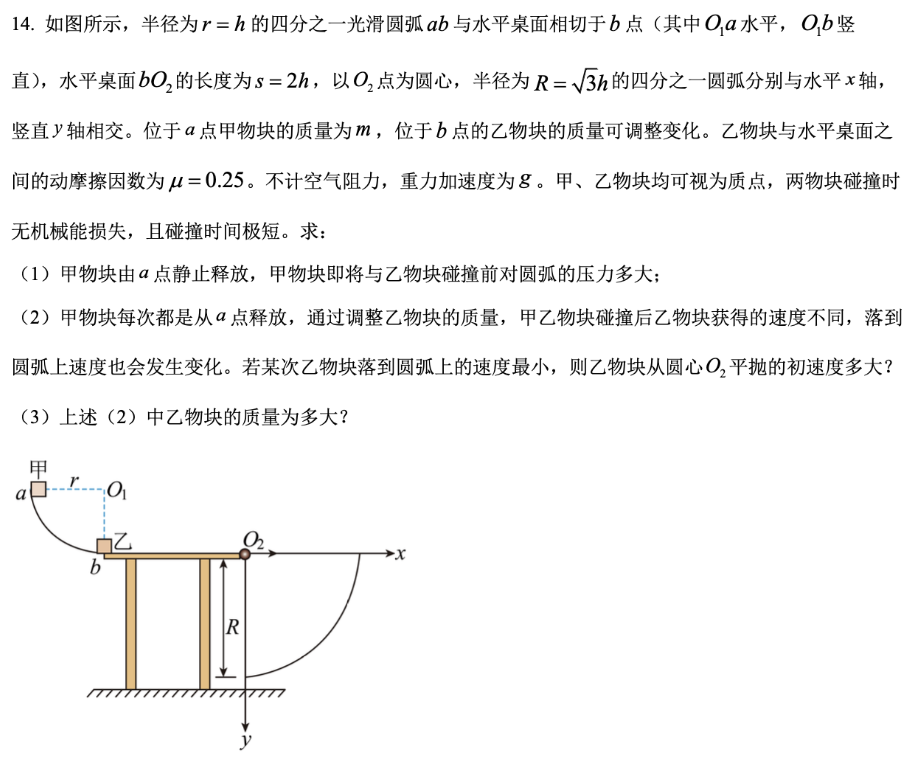
\includegraphics[width=0.95\textwidth,keepaspectratio]{./pictures/1.2-6.png}


\begin{itemize}
    \item 总结:\quad 在解方程组的时候,选择去消掉$t$直接得到$v = f(v_{0})$是非常困难的,事实上先解出$v = f(y)$求得最小的
          $y_{min}$,那么就可得到最小的$v_{ymin}$进而得到最小的$v = \sqrt{gh}$
\end{itemize}

\vspace{2em}


\subsection{2022-2023巴蜀中学下学期期末}
\subsubsection{I-13:电路中的变化量分析}
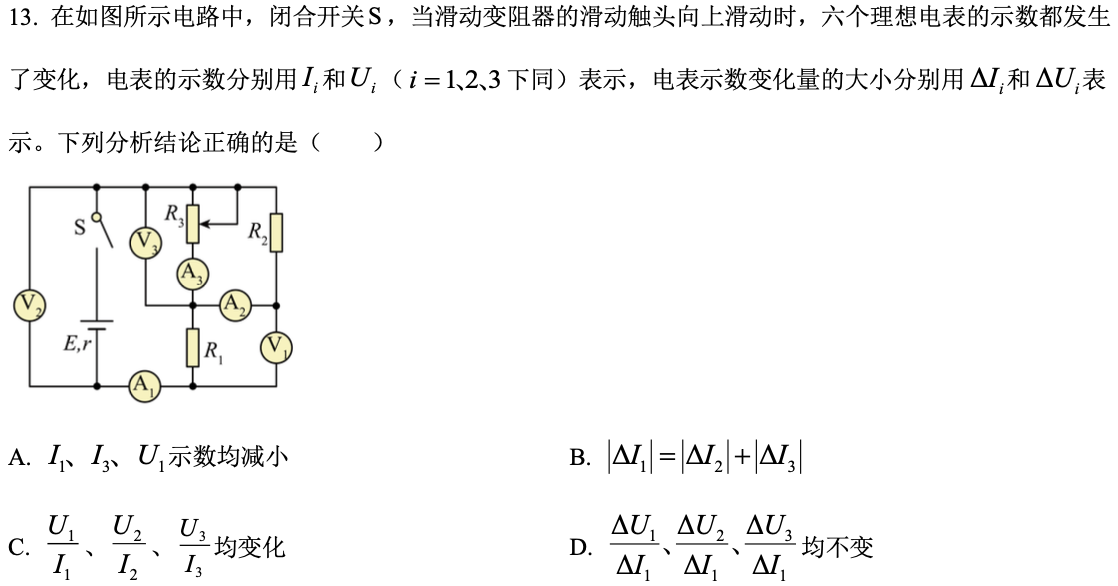
\includegraphics[width=0.95\textwidth,keepaspectratio]{./pictures/1.3-2.png}

\begin{itemize}
    \item 总结: \quad 最好写出回路的表达式$E = U_{2} + I_{1}r  \quad U_{3} = E - I_{1}(R_{1} + r)$
\end{itemize}

\vspace{2em}

\subsubsection{II-2:电路的测量误差}
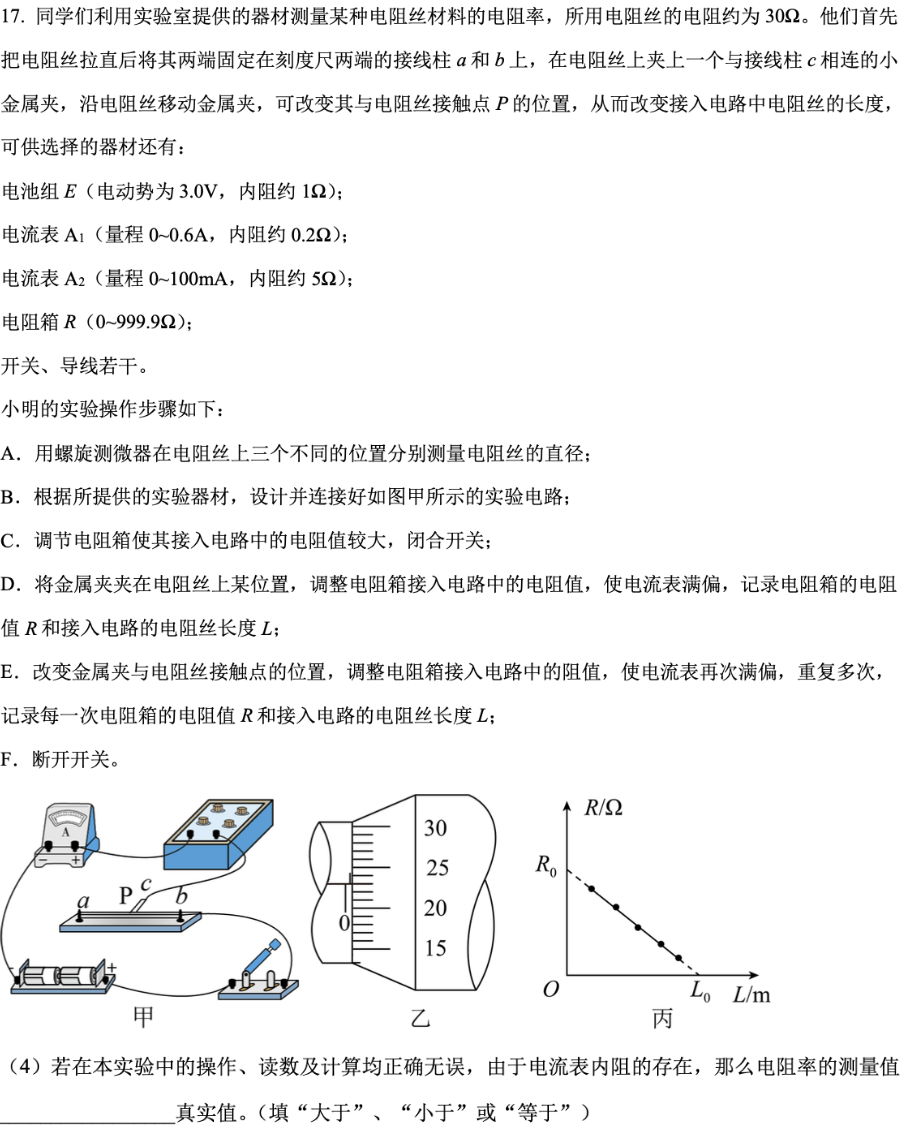
\includegraphics[width=0.95\textwidth,keepaspectratio]{./pictures/1.3-3.png}

\begin{itemize}
    \item 总结:\quad 官解结果正确但是思路奇怪,$R_{0}$会发生变化,存在电流表内阻时
          $$
              R_{0} = \frac{E}{I} - r
          $$
          所以$R_{0}$测量值偏小,但事实上实验步骤并不直接得到$R_{0}$,而是通过延长线的方式,因此$L_{0}$并非不变化的

          $$
              R_{i} = \frac{E}{I_{满偏}} - r -\frac{4\rho}{\pi d^{2}} L_{i}
          $$

          实验的测量值是准确的,因此忽略电流表内阻与仅仅是将直线向下移动,并不影响斜率,所以结果是等于
\end{itemize}

\vspace{2em}

\subsection{2022-2023南开中学高一下期末}
\subsubsection{I-6:光的几何表示问题}
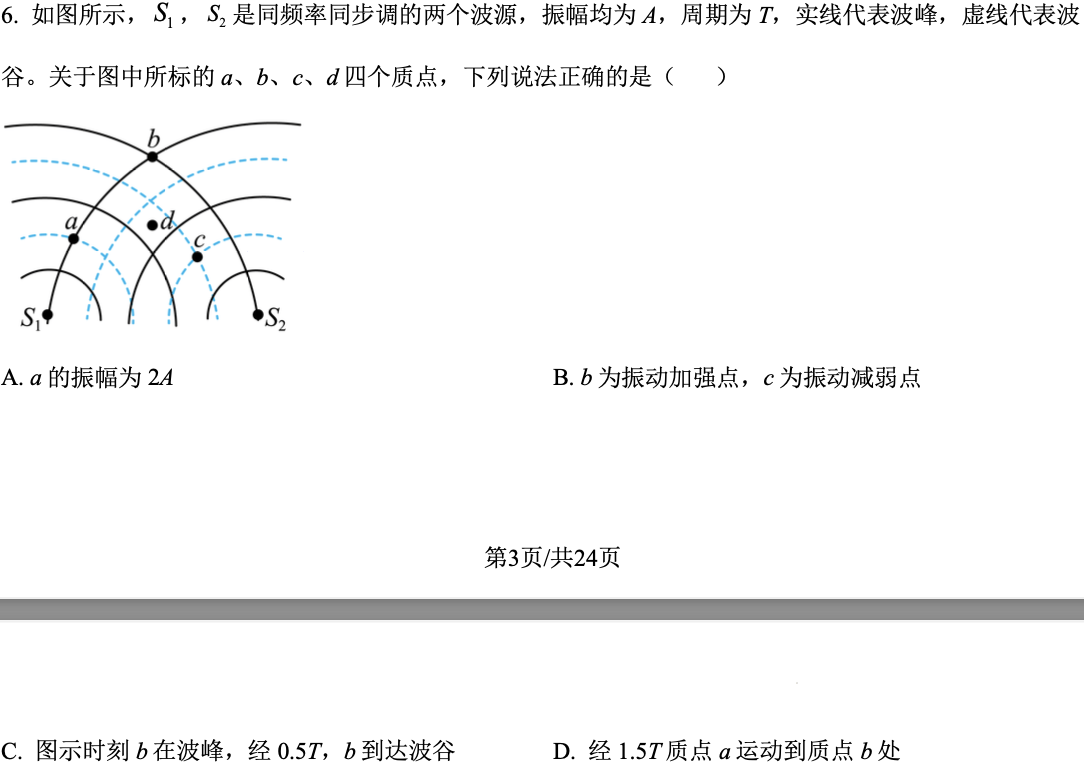
\includegraphics[width=0.95\textwidth,keepaspectratio]{./pictures/1.4-1.png}

\begin{itemize}
    \item 正解:\quad $C$
    \item 总结:\quad 此为光波的另一种表现方式,同时\textbf{振动加强点包括波峰叠加和波谷叠加},D选项,质点$a$实际仅在平衡位置振动,并不产生其它方向的位移
\end{itemize}

\vspace{2em}


\subsubsection{I-8:单摆+受迫振动}
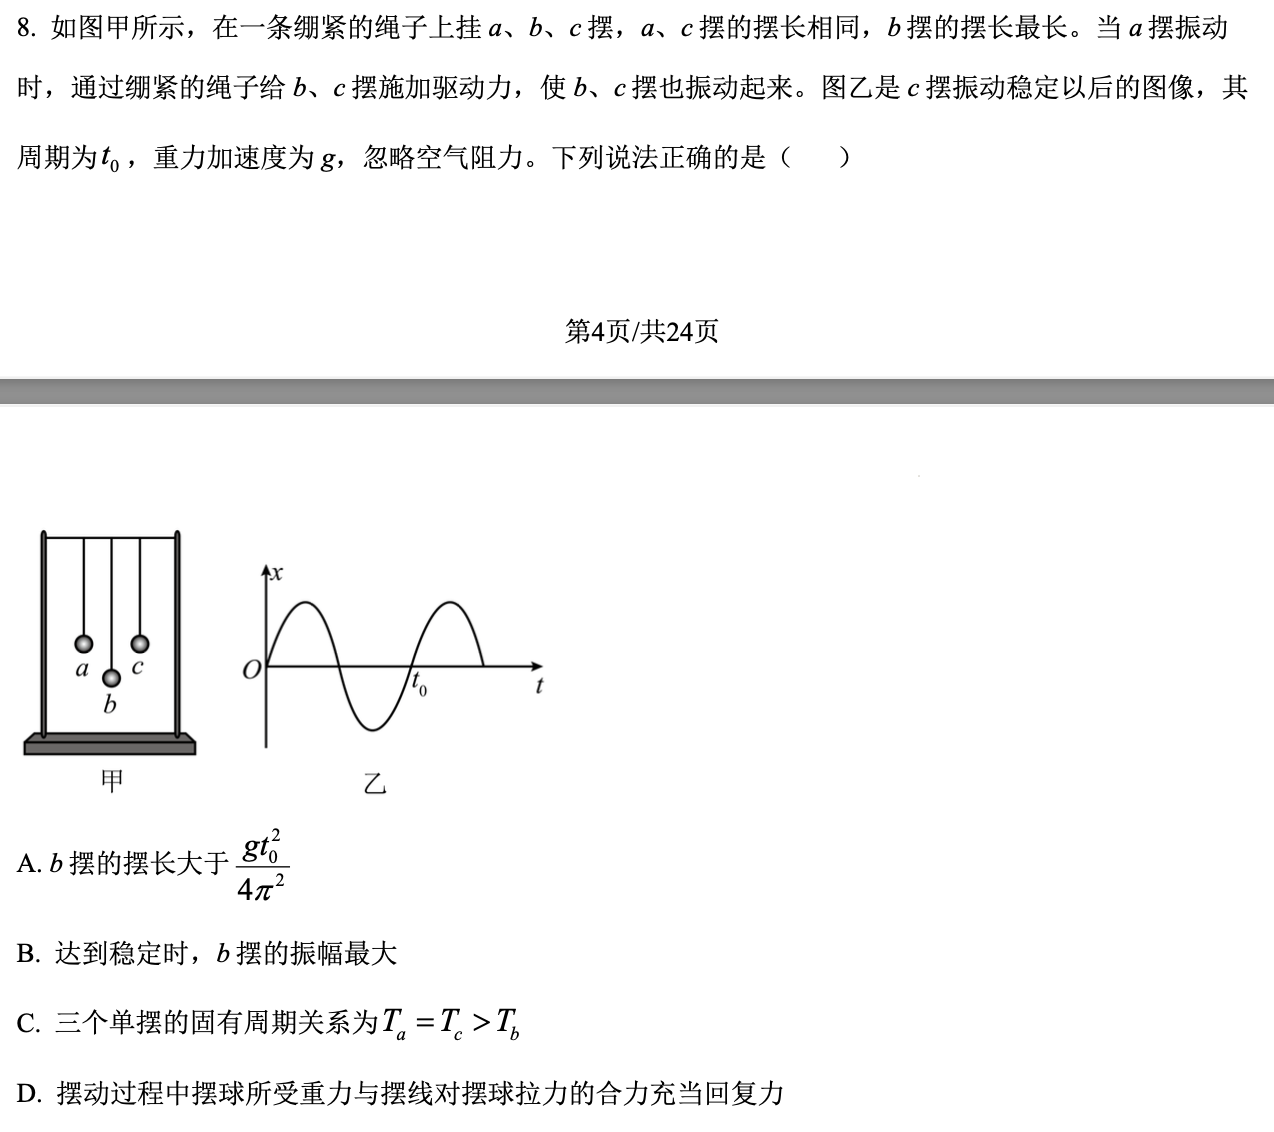
\includegraphics[width=0.95\textwidth,keepaspectratio]{./pictures/1.4-2.png}

\begin{itemize}
    \item 正解:\quad $A$
    \item 总结:\quad 单摆周期公式死记硬背,受迫振动:在周期性外力的持续作用下而进行的振动称为\textbf{受迫振动},振动稳定后齐\textbf{频率}等于外力驱动频率
          $$
              T = 2 \pi \sqrt{\frac{L}{g}}
          $$

          \begin{itemize}
              \item[]
                  \begin{proof}
                      证明运动为简谐运动,仅需证明回复力$F = -kx$(多次进行小量近似,很简单)\\
                  \end{proof}
              \item[]
                  \begin{proof}
                      证明简谐运动的周期(更复杂的方法请参考朗道等高阶解法)
                      \begin{align*}
                          F = -\frac{mg}{L} \vdot x                                               & = m \dv[2]{x}{t}           \\
                          \dv[2]{x}{t} + \frac{g}{L}x                                             & = 0                        \\
                          \text{令} \quad \omega                                                   & = \sqrt{\frac{g}{L}}       \\
                          \dv[2]{x}{t} + \omega^{2}x                                              & = 0                        \\
                          \text{特征根方程} \quad r^{2} = \omega^{2} \quad r                           & = \pm \omega i             \\
                          x = C \sin{(\omega t + \phi)} \quad \lra \quad T = \frac{2 \pi}{\omega} & = 2 \pi \sqrt{\frac{L}{g}}
                      \end{align*}
                  \end{proof}
          \end{itemize}
\end{itemize}

\begin{figure}[h]
    \centering
    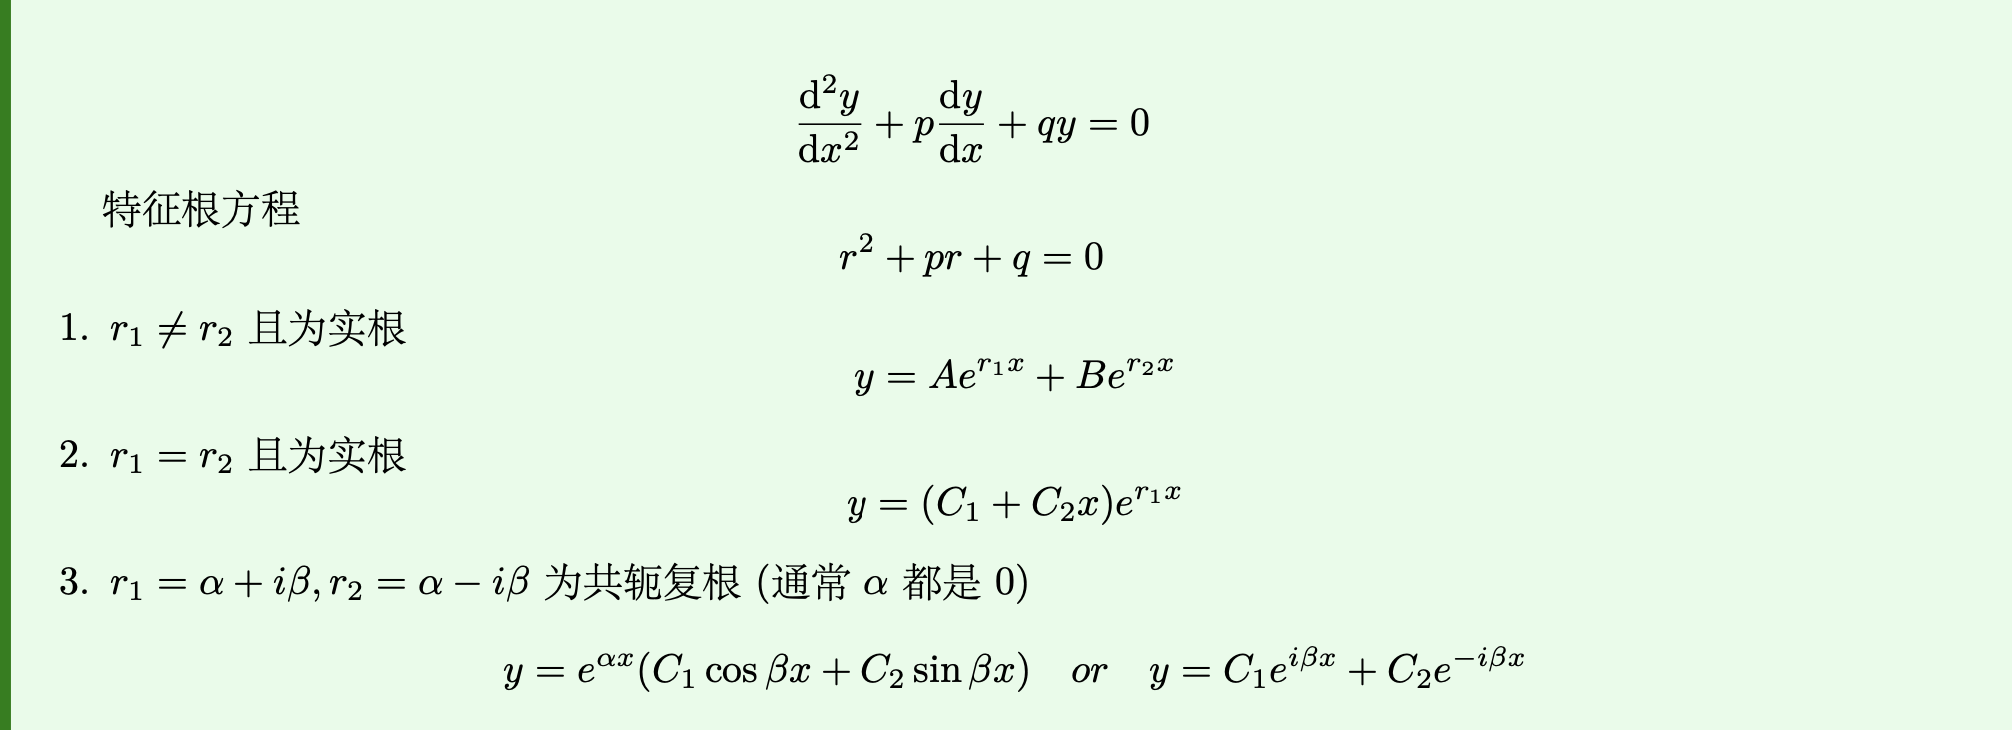
\includegraphics[width=\textwidth,keepaspectratio]{./pictures/1.4-3.png}
\end{figure}

\vspace{2em}

\subsubsection{I-10:折射率问题}
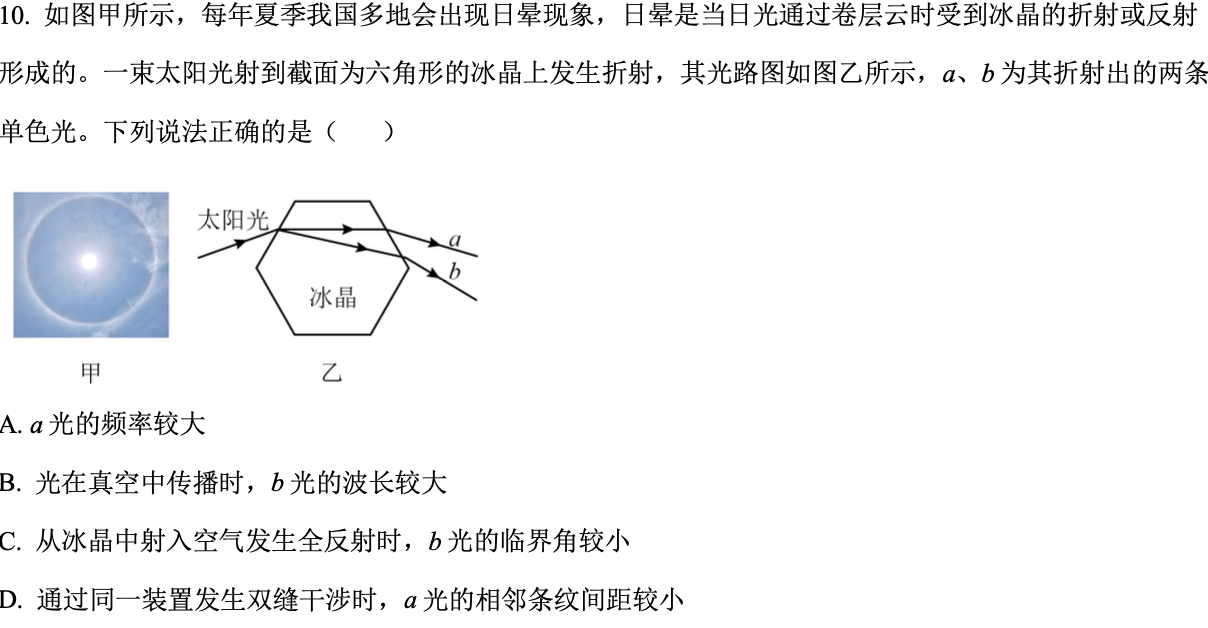
\includegraphics[width=0.95\textwidth,keepaspectratio]{./pictures/1.4-4.png}

\begin{itemize}
    \item 正解:\quad $C$
    \item 总结:\quad
          \begin{itemize}
              \item 光的\textbf{频率}$\nu$是本质属性,在任何介质下传播都不发生改变
              \item 同一介质中不同频率的光,\textbf{其折射率随频率单调递增}
              \item 同一光在不同介质的折射率不同
          \end{itemize}
    \item 扩展:\quad
          \begin{formal}
              符号说明

              \begin{tabular}{|c|c|c|c|c|c|c|c|c|c|}
                  \hline
                  频率  & 折射率 & 速度  & 临界角 & 波长        & 动量  & 干涉            & 能量            & 逸出功     & 逃逸光子动能  \\
                  \hline
                  $f$ & $n$ & $v$ & $C$ & $\lambda$ & $p$ & $\triangle x$ & $\varepsilon$ & $w_{0}$ & $E_{k}$ \\
                  \hline
              \end{tabular}

              \vspace*{2em}

              \begin{itemize}
                  \item 同一介质中不同频率的光

                        \vspace*{1em}
                        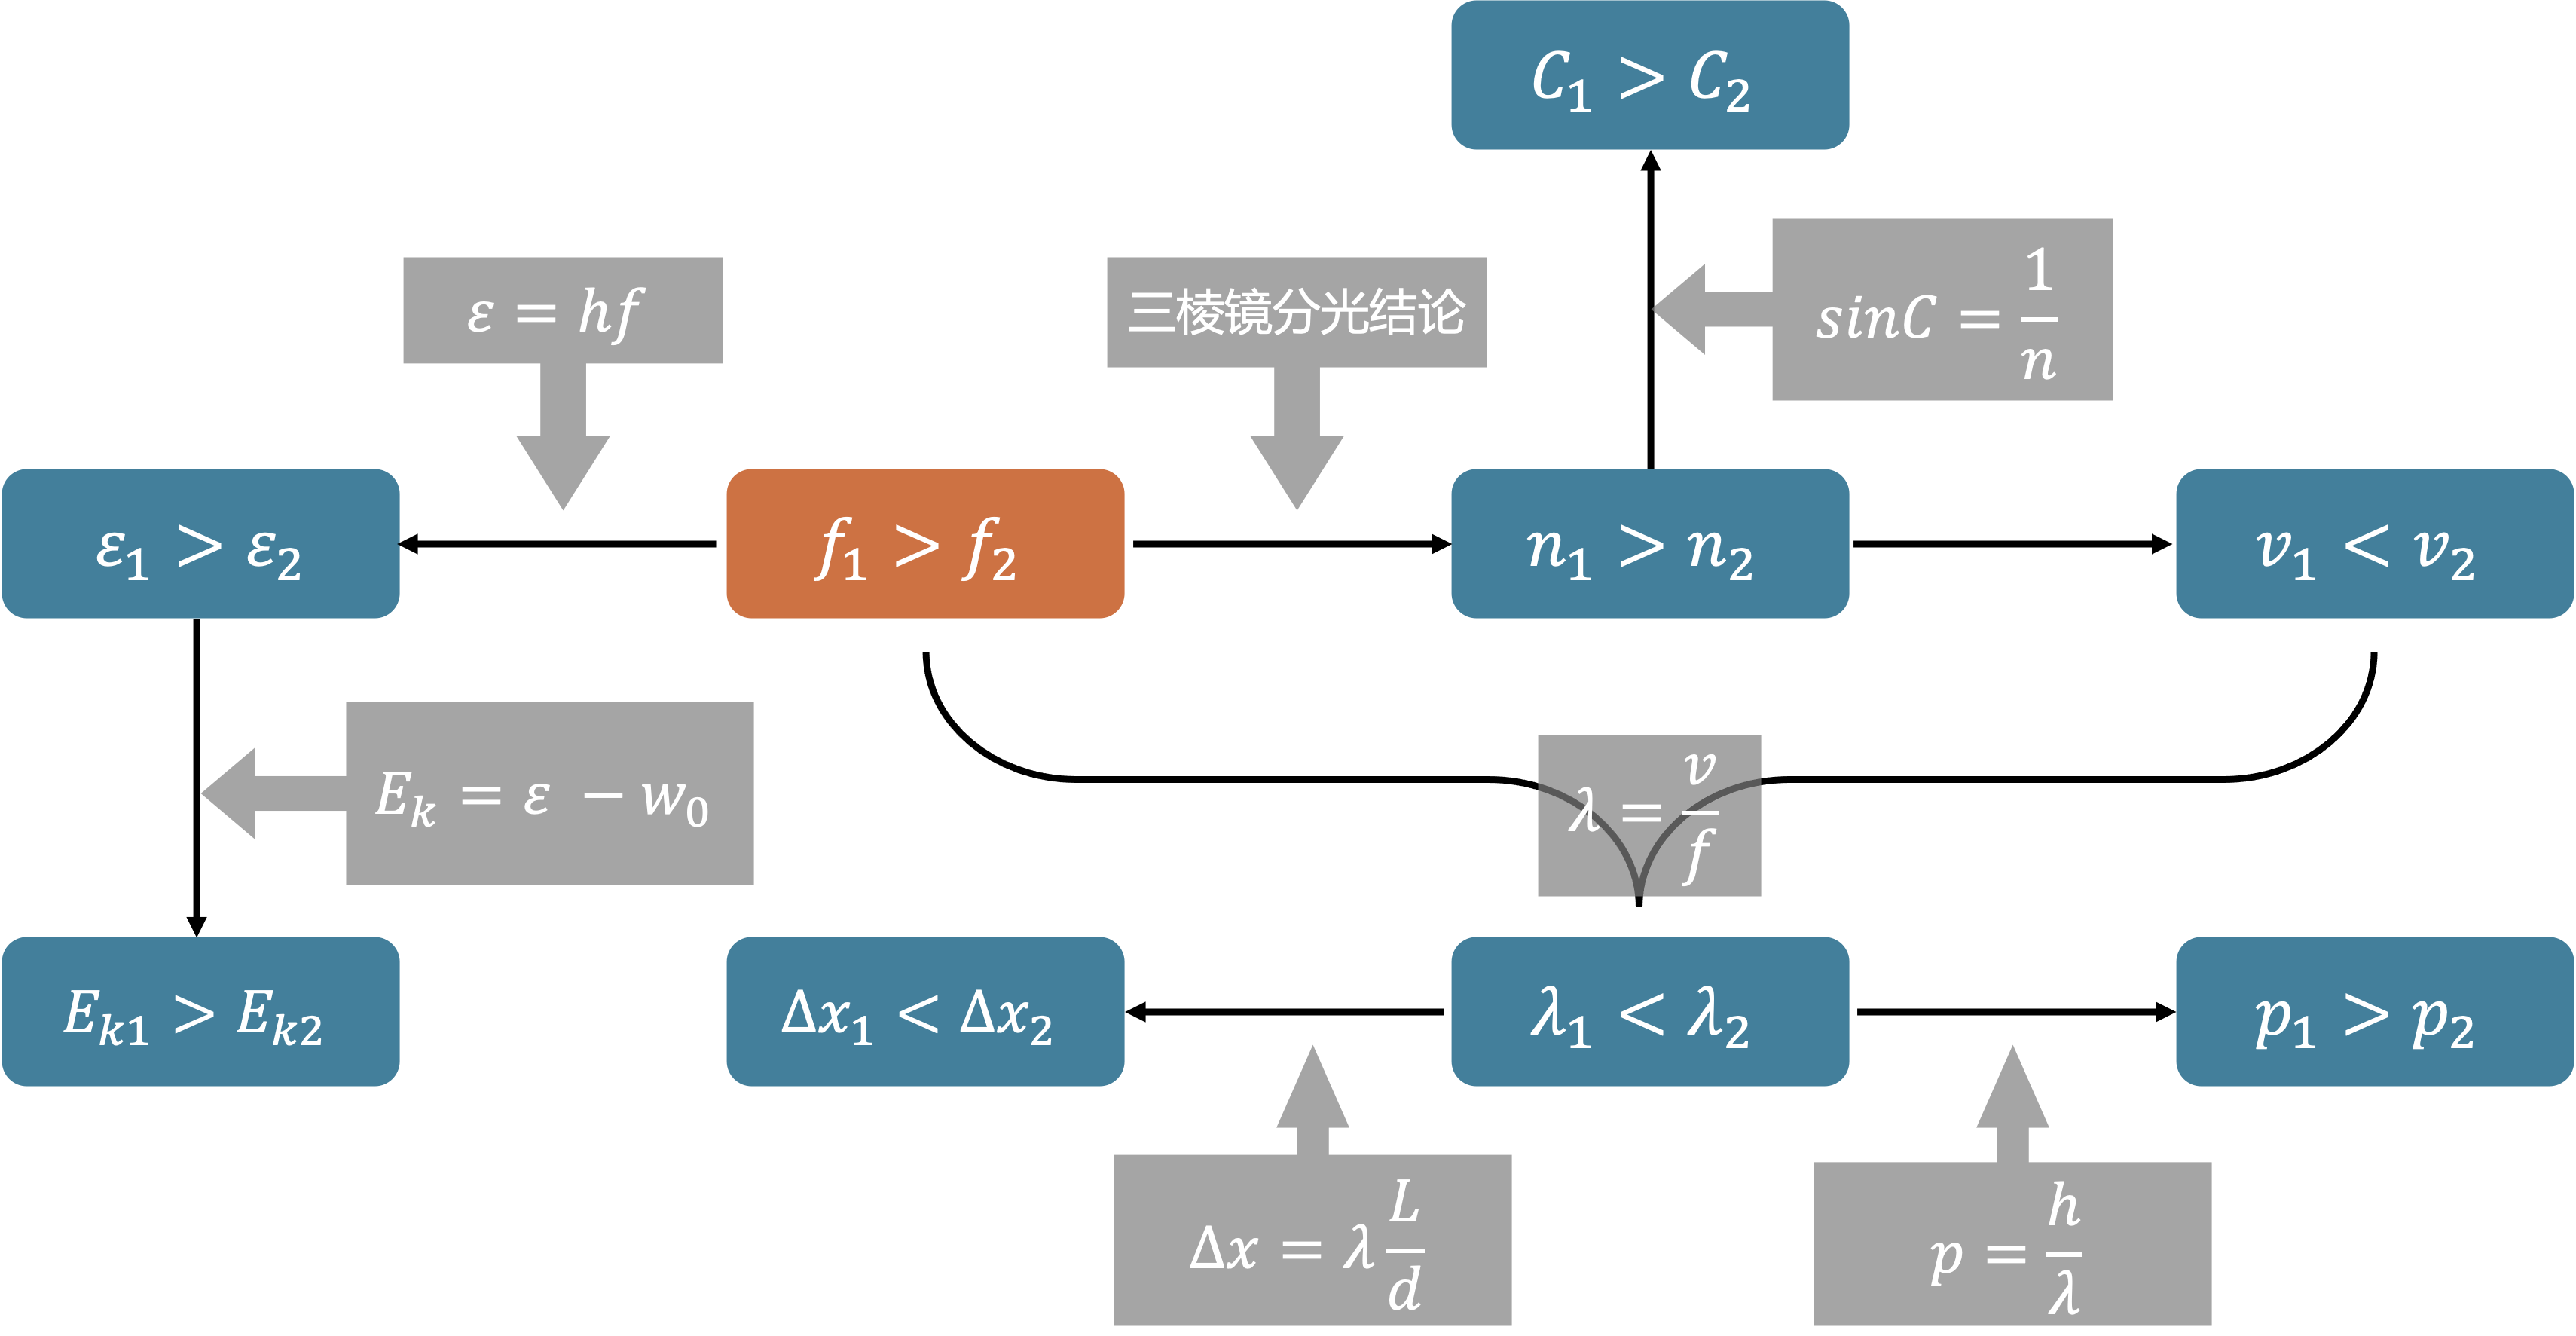
\includegraphics[width=40em,keepaspectratio]{./pictures/1.4-5.png}

                        \vspace*{2em}

                  \item 同一频率的光在不同介质(下标表示不同介质中)中

                        \vspace*{1em}
                        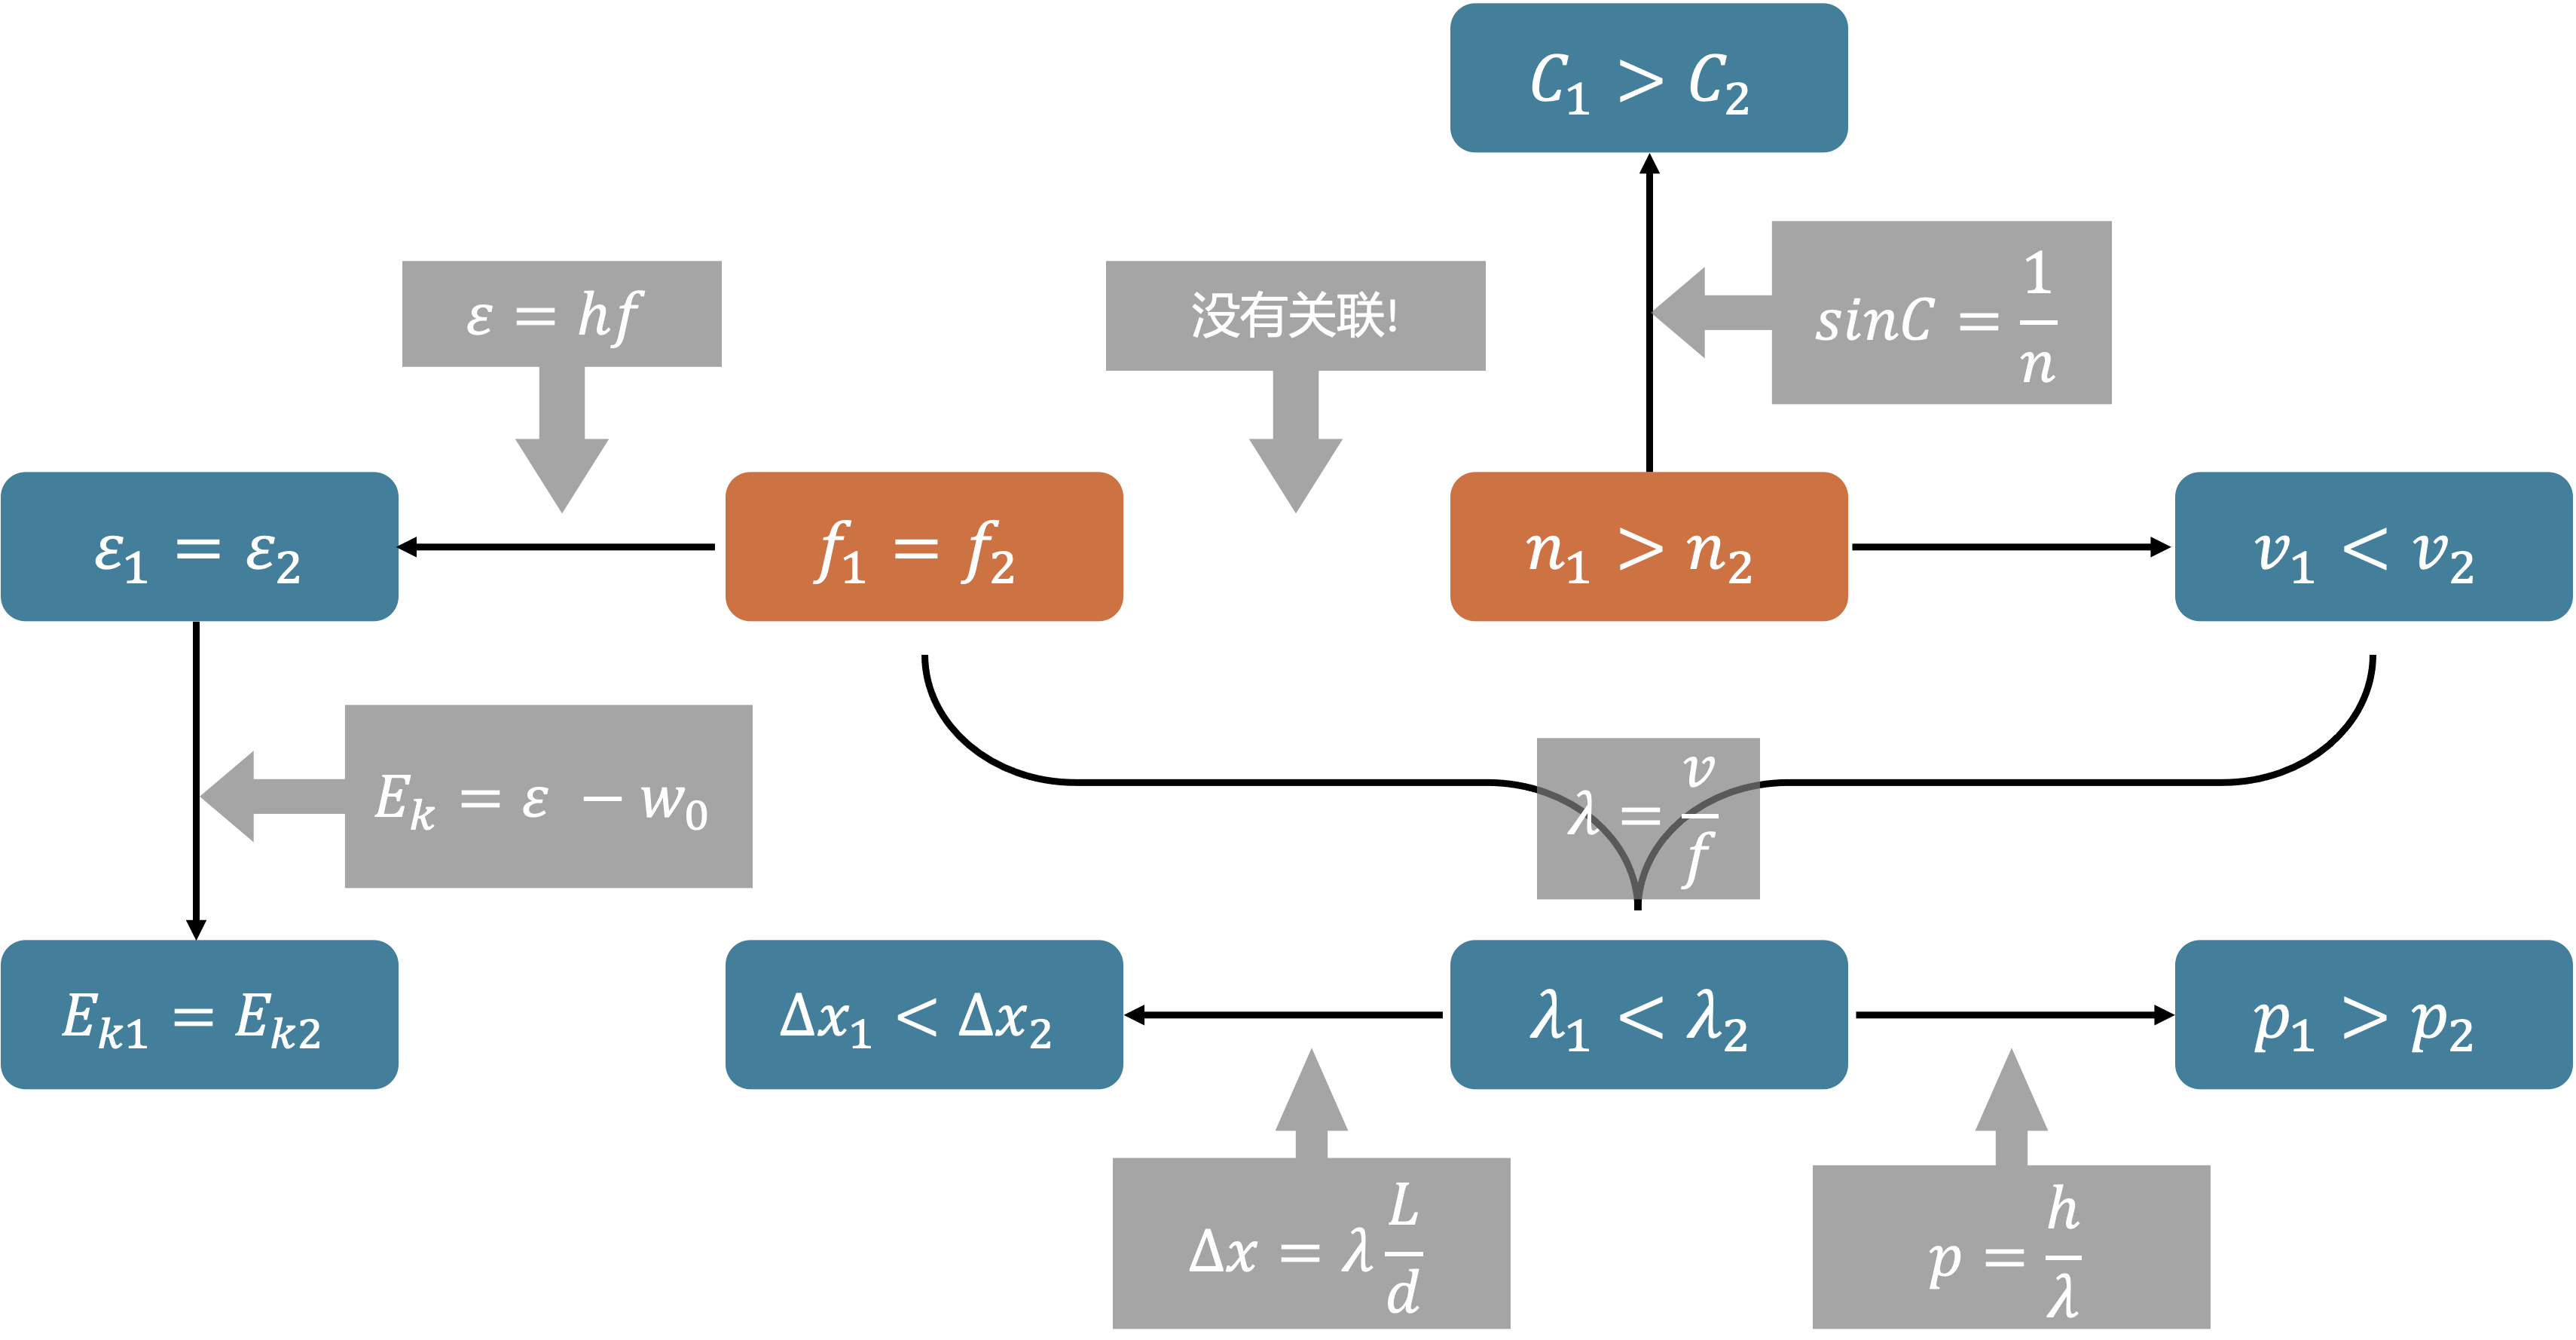
\includegraphics[width=40em,keepaspectratio]{./pictures/1.4-6.png}
              \end{itemize}
          \end{formal}
\end{itemize}

\vspace{2em}

\subsection{2022-2023育才中学期末模拟题(六)}
\subsubsection{II-3:水平初动量不为0的杆相互作用模型}

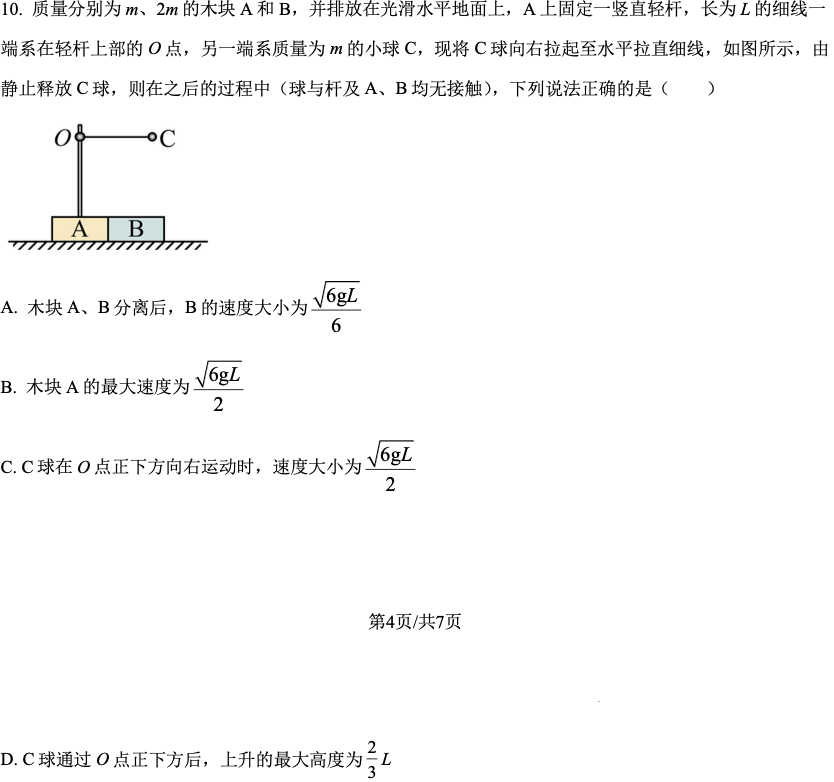
\includegraphics[width=0.95\textwidth,keepaspectratio]{./pictures/1.5-1.png}

\begin{itemize}
    \item 正解:\quad $ABD$
    \item 总结:\quad 是一类通过杆相互作用的水平动量守恒模型,但是注意系统初动量不为0
\end{itemize}

\vspace{2em}

\subsection{2022-2023育才中学期末模拟题(三)}
\subsubsection{I-6:调和定律-新颖题目}

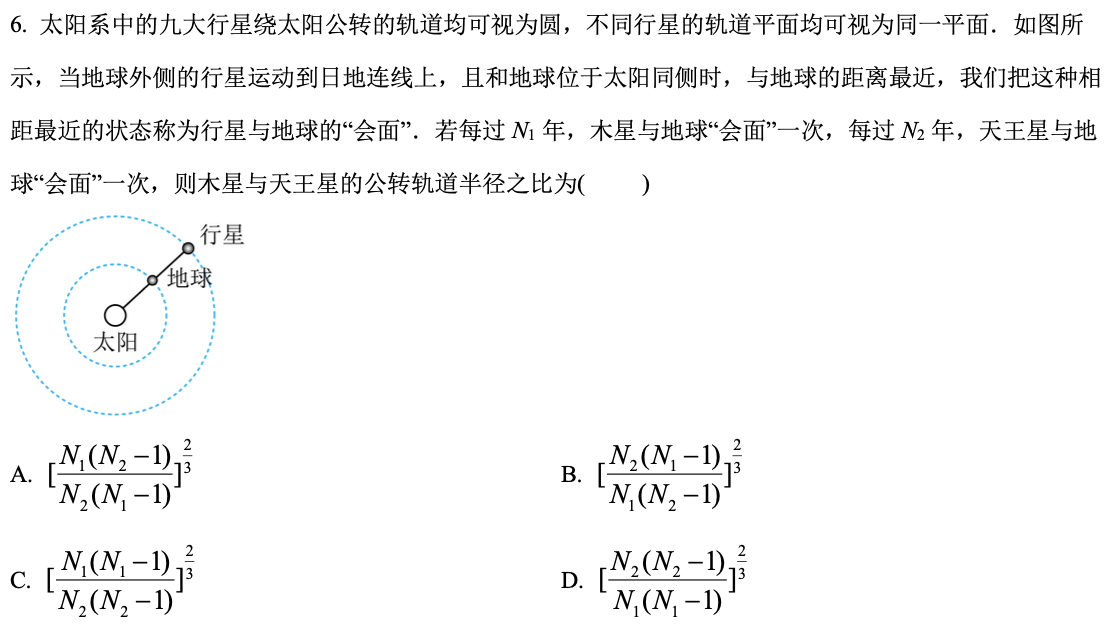
\includegraphics[width=0.95\textwidth,keepaspectratio]{./pictures/1.5-2.png}

\begin{itemize}
    \item 正解:\quad $A$
    \item 总结:\quad 注意理解一年的意义
\end{itemize}

\subsubsection{II-3:连续弹碰(牛顿摆)}

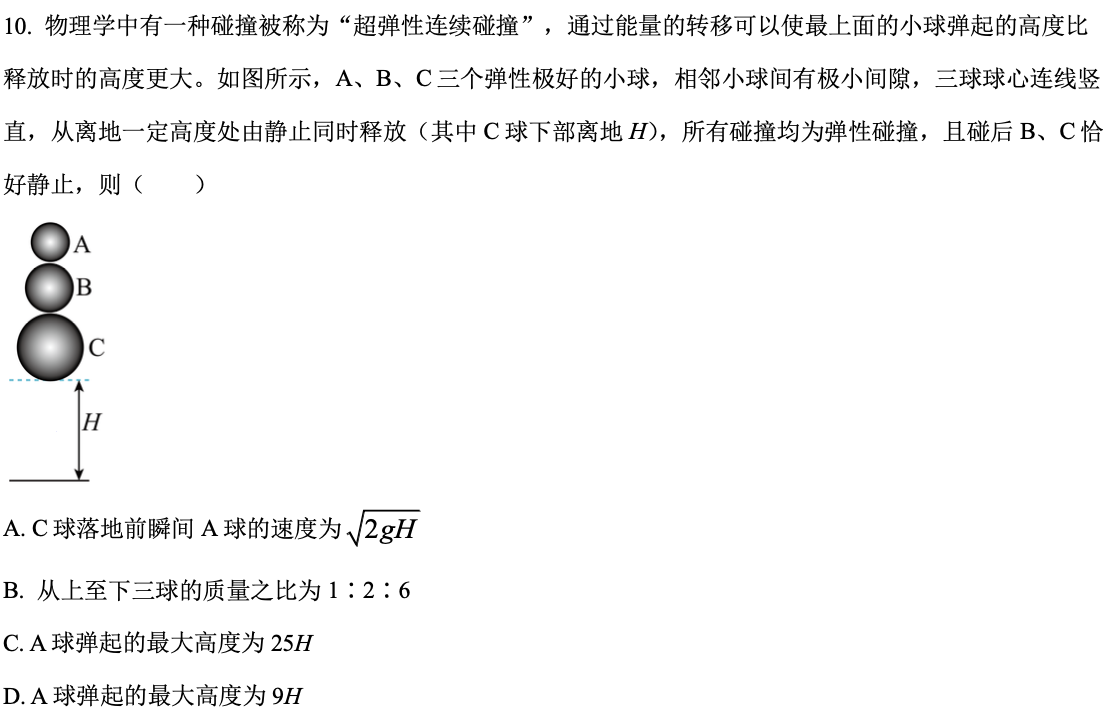
\includegraphics[width=0.95\textwidth,keepaspectratio]{./pictures/1.5-3.png}

\begin{itemize}
    \item 正解:\quad $ABD$
    \item 总结:\quad 逐个分析即可
    \item 扩展:\quad 牛顿摆的分析方法也是先研究瞬时碰撞的两个物体,并进行传递
\end{itemize}

\vspace{2em}

\subsection{2022-2023一中高一下期末}
\subsubsection{III-1:折射率实验}

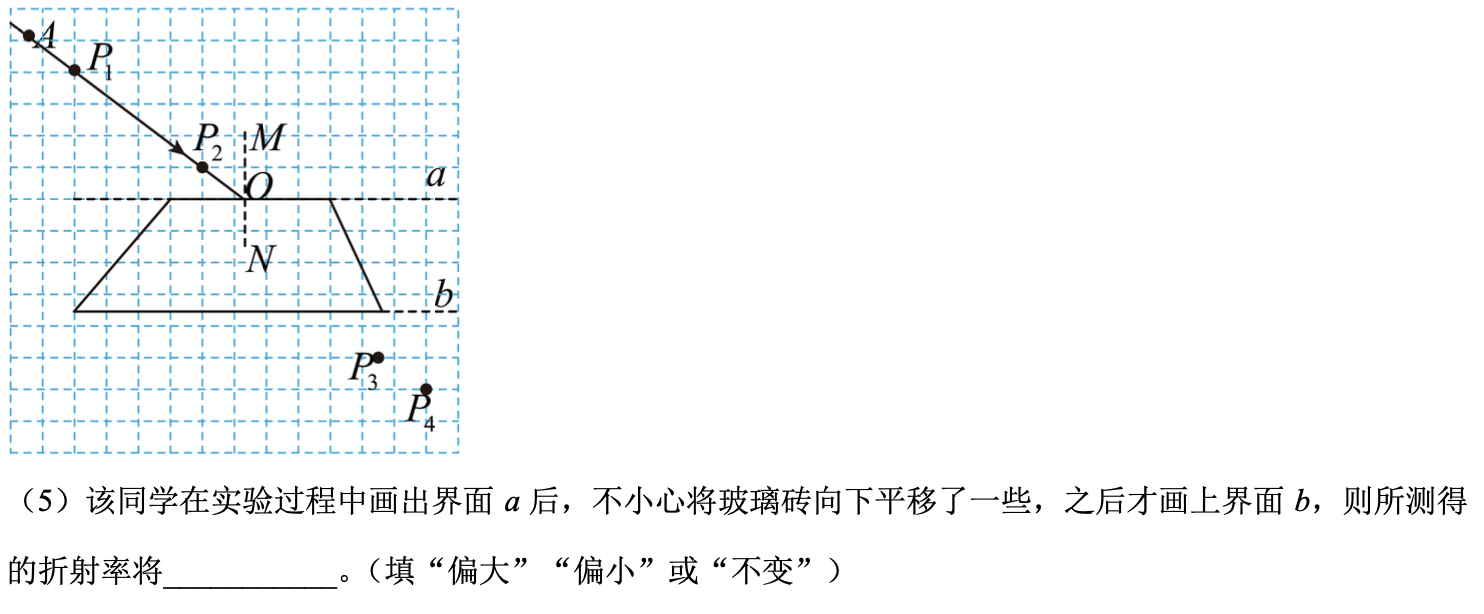
\includegraphics[width=0.95\textwidth,keepaspectratio]{./pictures/1.6-1.png}

\begin{itemize}
    \item 正解:\quad 偏小
    \item 总结:\quad 玻璃砖整体平移,非平行玻璃砖的测量是准确的;
          其他情况$d_{\text{画}}$\,$d_{\text{玻}}$的大小关系与$n_{\text{测}}$\,$n_{\text{真}}$相反    \\
          此题中由于将玻璃下移后才画上下边界,因此$d_{\text{画}} > d_{\text{真}} \quad \lra \quad n_{\text{测}} < n_{\text{真}}$
\end{itemize}

\vspace{2em}

\subsection{2024育才高一下期末}
\subsubsection{I-1: 飞机功率计算问题}

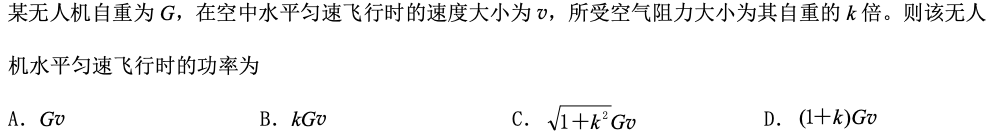
\includegraphics[width=0.95\textwidth,keepaspectratio]{./pictures/1.7-1.png}


\begin{itemize}
    \item 正解:\quad $A$
    \item 总结:\quad 飞机水平匀速运动过程中,发动机不需要提供向上的力,这部分力由升力提供
\end{itemize}

\subsubsection{III-1: 纸带钩码研究动能定理}
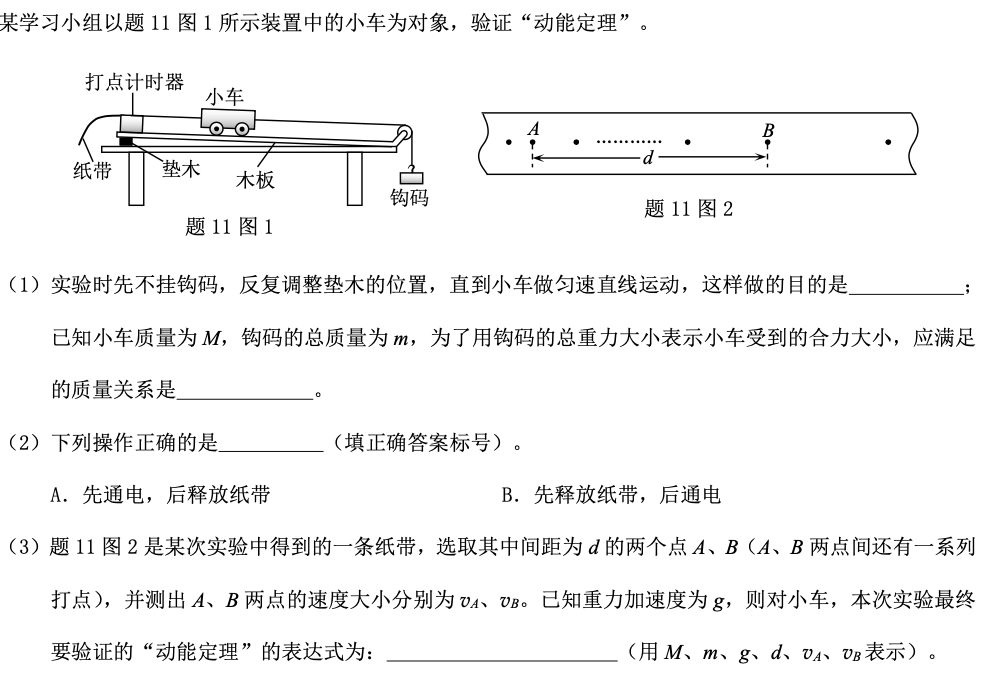
\includegraphics[width=0.95\textwidth,keepaspectratio]{./pictures/1.7-2.png}

\begin{itemize}
    \item 正解:\quad 
    
    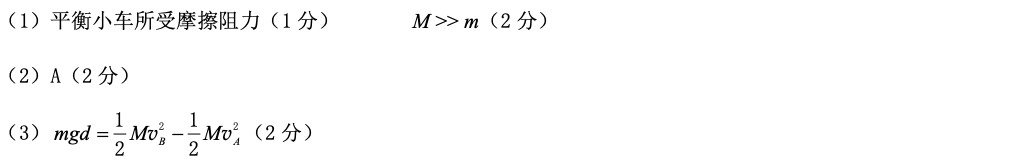
\includegraphics[width=0.85\textwidth,keepaspectratio]{./pictures/1.7-3.png}

    \item 总结:\quad 先通电再释放;钩码总质量远小于小车质量
    
    \hspace{3.2em}$T = Ma \quad mg - T = ma \quad a = \frac{m}{m+M}g \lra T = \frac{mM}{m+M}g$

    \hspace{3.2em}上下同时除以$M \lra$$T = \frac{m}{\frac{m}{M}+1}g$,因此当$m$远小于$M$时$T = mg$
\end{itemize}

\vspace{2em}

\section{高二}

\subsection{机械振动专题}
\subsubsection{I-1:起振方向未知的多解问题}
一个弹簧振子沿$x$做简谐运动,平衡位置在坐标原点,振幅为$0.2m$.$t= 0$时振子的位移为$-0.1m$,$t = 0.5s$时位移第一次为$0.1m$,则振子的周期可能是
$$
    A. 1s   \hspace{10em}    B. 1.5s      \hspace{10em}    C. 2s      \hspace{10em}    D. 3s
$$

\begin{itemize}
    \item 正解:\quad $AD$
    \item 总结:\quad 起振方向未知,存在多解
          \begin{align*}
              y & = 0.2\sin{(\omega t + \varphi)}                            \\
              t & = 0  \quad  \sin{\varphi} = -\dfrac{1}{2} \quad \lra \quad
              \begin{cases}
                  \varphi = - \dfrac{\pi}{6} \\
                  \,                         \\
                  \varphi = - \dfrac{5\pi}{6}
              \end{cases}                                     \\
              t & = 0.5s \quad \sin{0.5 \omega  + \varphi } = \dfrac{1}{2}   \\
                & \begin{cases}
                      \dfrac{\omega}{2} - \dfrac{\pi}{6} = \dfrac{\pi}{6} \\
                      \,                                                  \\
                      \dfrac{\omega}{2} - \dfrac{5\pi}{6} = \dfrac{\pi}{6}
                  \end{cases}
              \quad \lra  \quad
              \begin{cases}
                  \omega = \dfrac{2\pi}{3} \quad \lra \quad T = \dfrac{2\pi}{\omega} = 3s \\
                  \,                                                                      \\
                  \omega = 2\pi \quad \lra \quad T = \dfrac{2\pi}{\omega} = 1s
              \end{cases}
          \end{align*}

    \item 扩展:\quad

          造成波的多解性的三大原因:
          \begin{itemize}
              \item \textbf{波的周期性:}\hspace{1em}
                    $\begin{cases}
                            \text{时间周期性:时间间隔}\triangle t \text{与周期} T \text{的关系不明确} \\
                            \text{空间周期性:波传播距离}\triangle x \text{与波长} \lambda \text{的关系不明确}
                        \end{cases}$

              \item \textbf{波的双向性:}\hspace{1em}
                    $\begin{cases}
                            \text{传播方向双向性:波的传播方向不确定} \\
                            \text{振动方向双向性:质点振动方向不确定}
                        \end{cases}$

              \item \textbf{波形隐含性:}\hspace{1em}
                    $\begin{cases}
                            \text{在波动问题中,有时只给出几个特殊点} \\
                            \text{(大多是两个特殊的点)的运动状态,其余信息均处于隐含状态}
                        \end{cases}$
          \end{itemize}

\end{itemize}

\vspace{2em}

\subsubsection{I-2:球面波干涉图像问题}
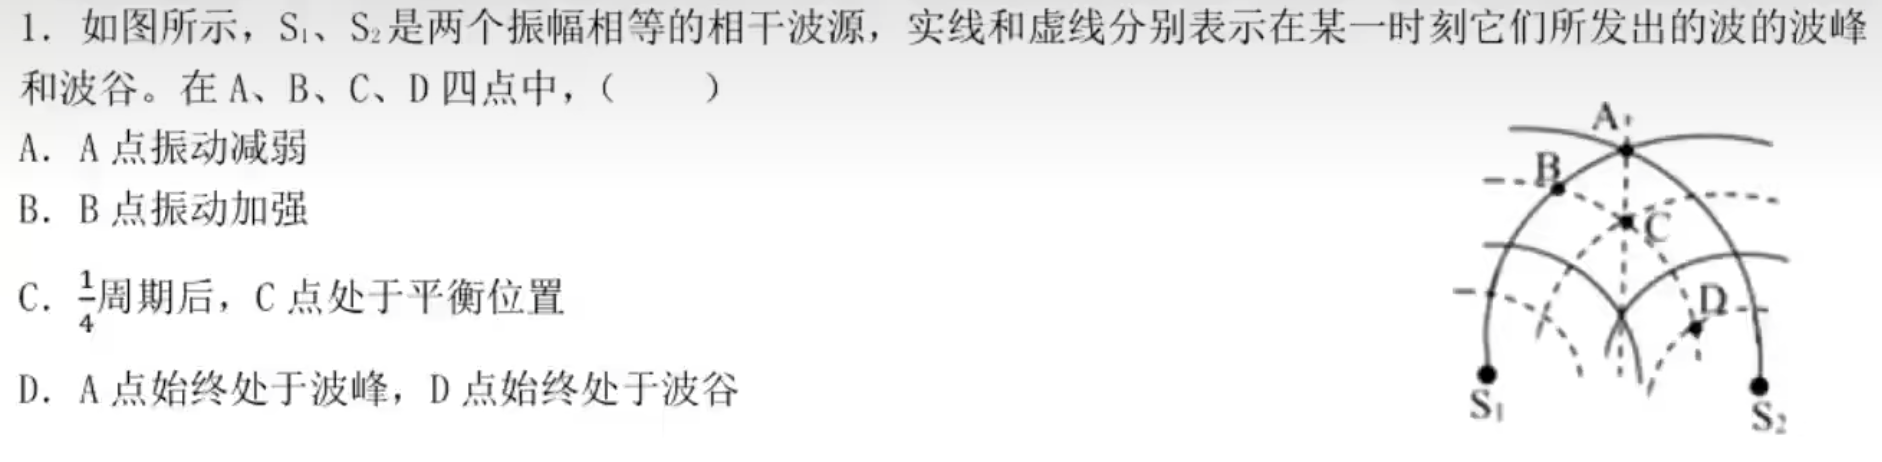
\includegraphics[width = 0.95\textwidth]{./pictures/2.1-1.png}

\begin{itemize}
    \item 正解:\quad $C$
    \item 总结:\quad C选项,c点为振动加强点,仅仅是振幅变大,并非不在平衡位置振动,研究$\frac{1}{T}$时间后
          的位置情况,是根据叠加波(周期不变)的传播来看,经过该时间后,波谷达到平衡位置,所以C选项正确
    \item 扩展:\quad 此类干涉图的所有振动加强点的连线是双曲线.有的此类图形未必是干涉图像,比如两个水波的叠各自具有不同的周期,因此某个点振动加强或减弱并非恒定
\end{itemize}

\begin{center}
    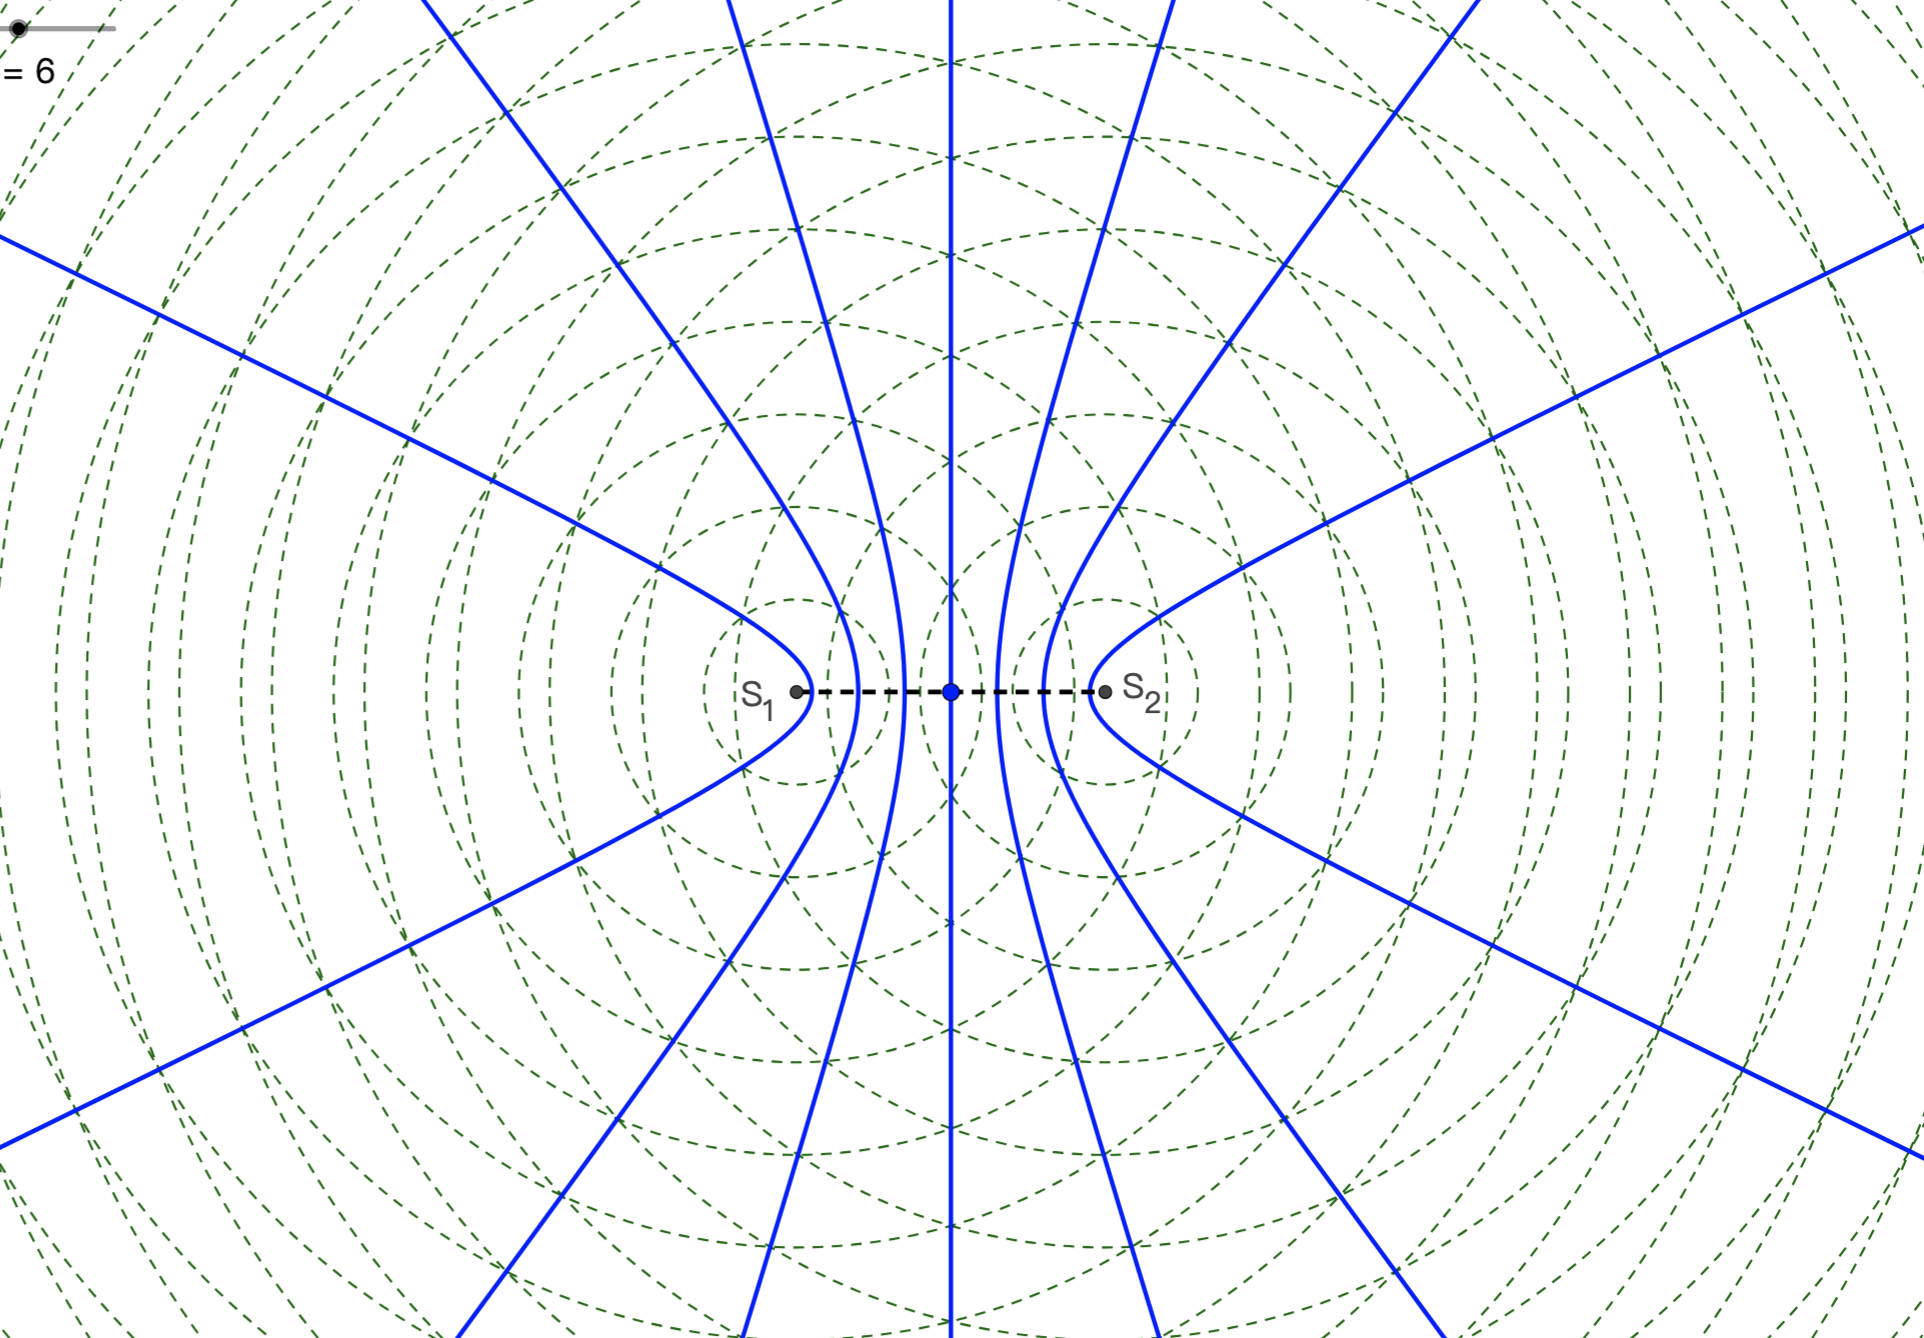
\includegraphics[width = 0.6\textwidth]{./pictures/2.1-2.png}
\end{center}

\vspace{2em}

\subsubsection{I-3:球面波非干涉图像问题}
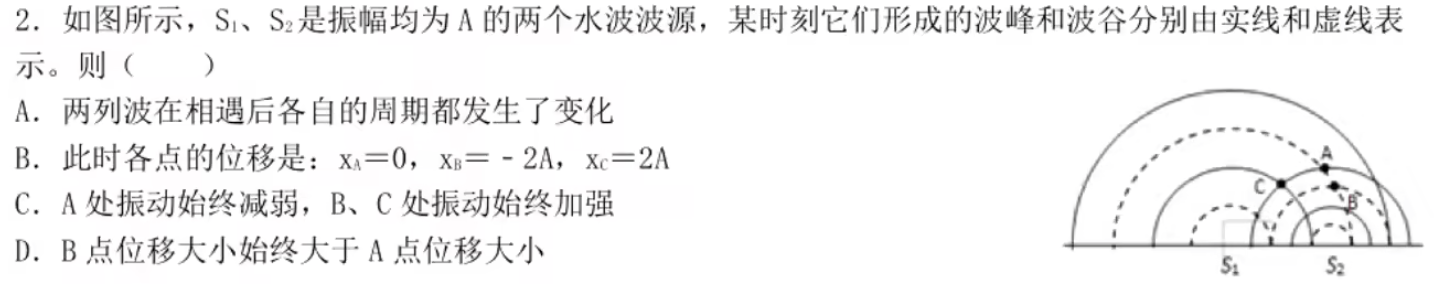
\includegraphics[width = 0.95\textwidth]{./pictures/2.1-6.png}

\begin{itemize}
    \item 正解:\quad $B$
    \item 总结:\quad 两个水波没有特定说明则是非相干波源,因此振幅的加强或减弱是非恒定的
\end{itemize}

\vspace{2em}

\subsubsection{I-4:折射率几何求解}
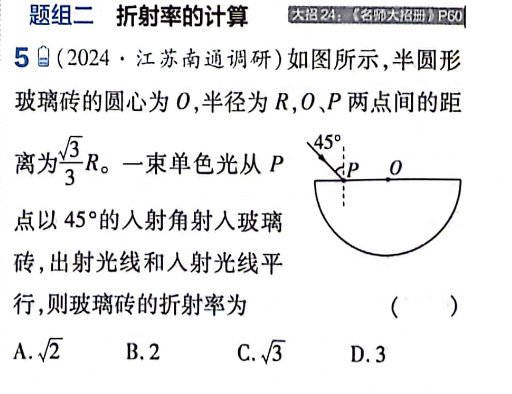
\includegraphics[width = 25em]{./pictures/2.1-9.png}

\begin{itemize}
    \item 正解:\quad $A$
    \item 总结:\quad 此类问题关键是寻找折射光线在圆弧的位置,因为要求出射光线与入射光线平行,因此两次折射情况应该完全一致$45^\circ \ra \gamma \quad \gamma \ra 45^\circ$.
          那么可以得出第二次折射处的情况也是一个水平面(至少法线方向和第一次折射的法线方向平行).于是可以得到第二次折射点恰为圆弧底,且法线在竖直方向上且过圆心.
    \item
\end{itemize}


\vspace{2em}

\subsubsection{II-1:平面波干涉图像问题}
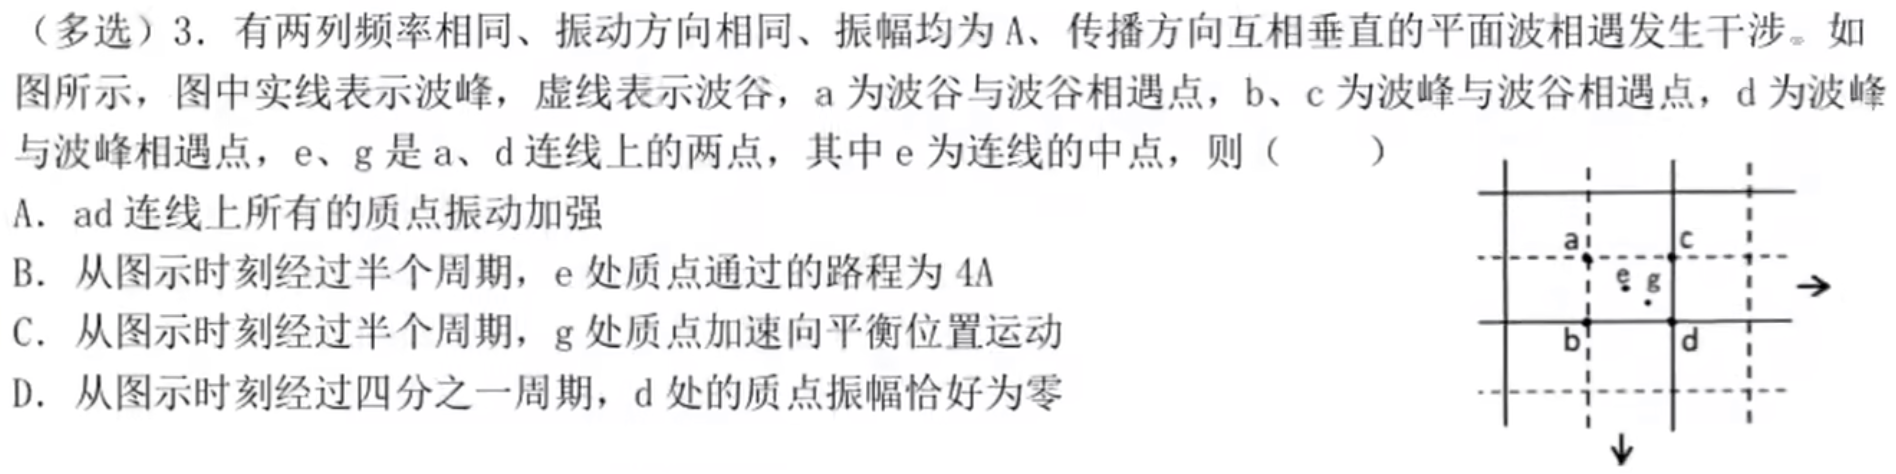
\includegraphics[width = 0.95\textwidth]{./pictures/2.1-3.png}

\begin{itemize}
    \item 正解:\quad $ABC$
    \item 总结:\quad
          \begin{itemize}
              \item[A.] 两个振幅加强点的连线上的所有点都是加强点.
              \item[B.] 简谐运动的结论,经过一个周期,质点(平衡位置或最大振幅位置)走过路程为4倍振幅.
                  经过半个周期,质点走过2倍振幅.在此选项中,质点$e$为加强点振幅为$2A$,经过半个周期,质点走过$2*2A = 4A$
              \item[C.] 运用简谐波的结论和同侧法判断振动方向(当然题目存在一定的语言上的细节,$g$减速到最大振幅后向平衡位置移动,加速度指向平衡位置)
              \item[D.] 题目考查的语言的艺术,可以描述$d$点所处位置为平衡位置,但是$d$点是振幅加强点不为$0$
          \end{itemize}
\end{itemize}

\vspace{2em}

\subsubsection{II-2:斜面弹簧组合体简谐振子}
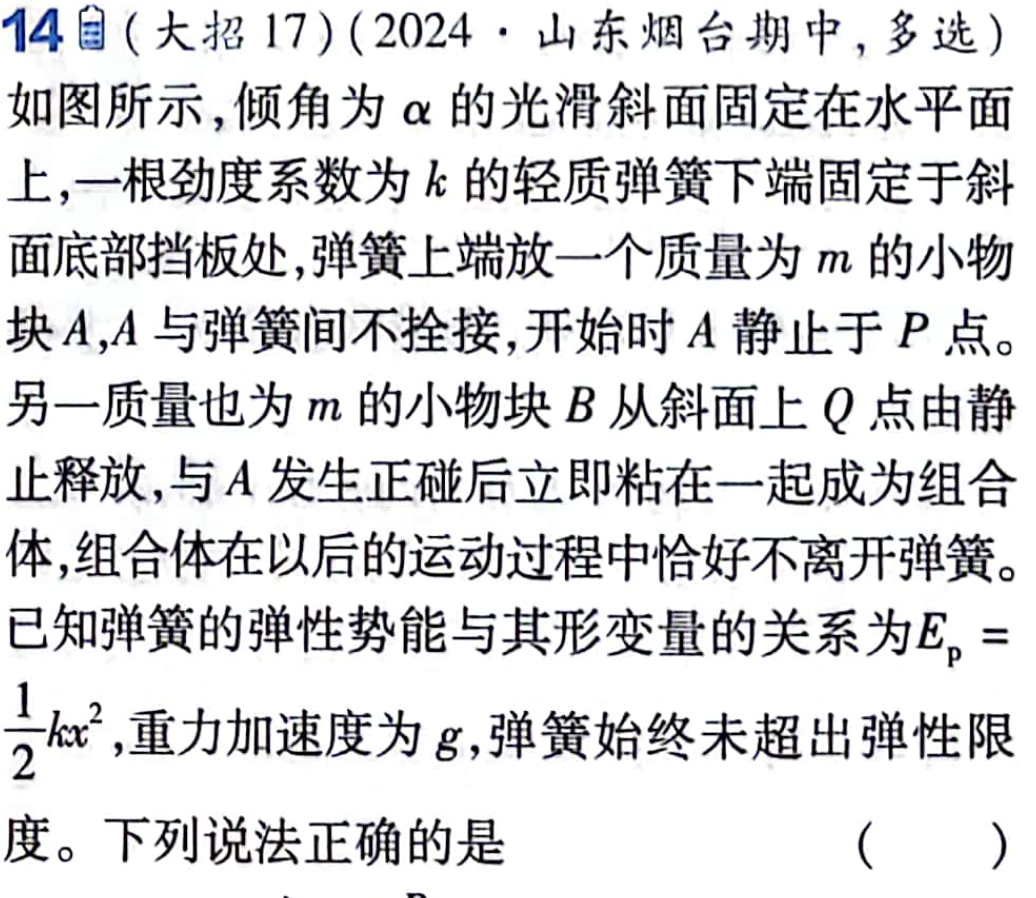
\includegraphics[width = 20em]{./pictures/2.1-7.png}
\hspace{2em}
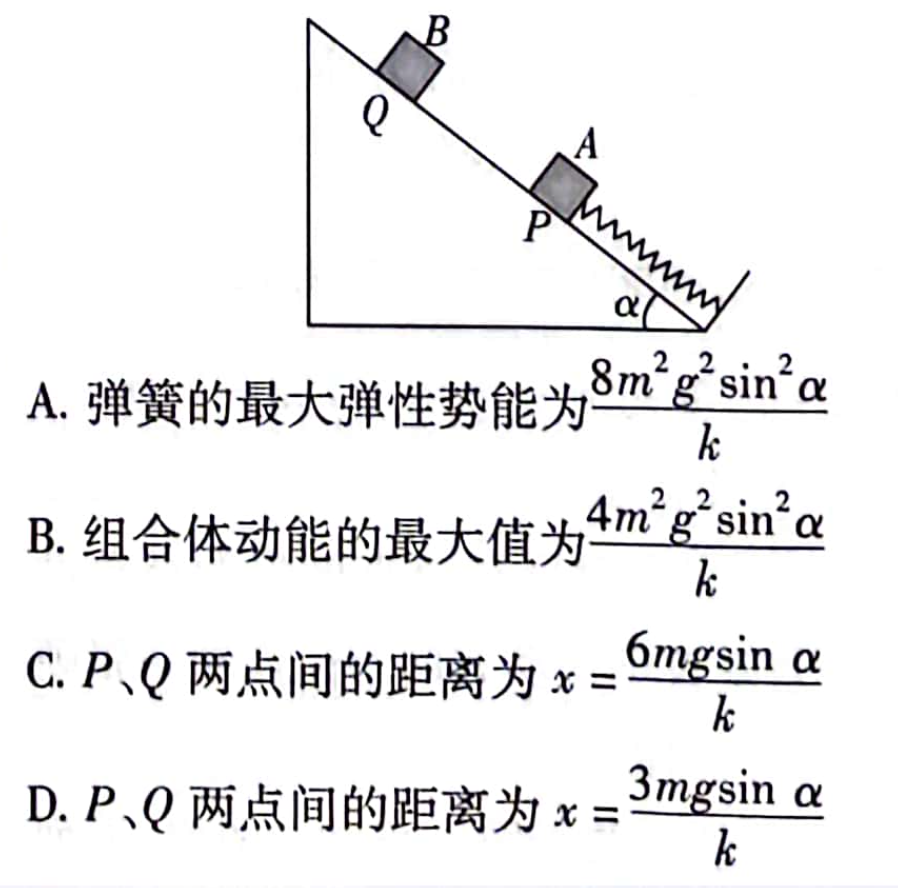
\includegraphics[width = 20em]{./pictures/2.1-8.png}

\begin{itemize}
    \item 正解:$AD$
    \item 总结:
          题目的过程较为复杂,我们需要理清每一个阶段
          \begin{enumerate}
              \item 初始阶段,物块$A$静止,弹簧被压缩至$x_{1} = \frac{mg\sin{\alpha}}{k}$
              \item 组合体阶段,题目的关键信息:组合体运动过程中\textbf{恰好}不离开弹簧,因此在恢复原长时组合体的速度为$0$.此时的回复力$F_{\text{回}} = 2mg\sin{\alpha}$(向下),
                    由简谐振动的性质,压缩到最大时的回复力大小也应该如此,因此$kx_{2} - 2mg\sin{\alpha} = 2mg\sin{\alpha} \quad \lra \quad x_{3} = \frac{4mg\sin{\alpha}}{k}$.

                    由此可得弹簧的最大弹性势能$ E_{pmax} = \frac{1}{2}kx_{2}^{2} = \frac{8m^{2}g^{2}\sin^{2}{\alpha}}{k} = 8J \quad (J = \frac{m^{2}g^{2}\sin^{2}{\alpha}}{k} )$

              \item 研究组合体最大的动能,显然我们需要找到谐振运动的平衡点即$F_{\text{回}} = 0$的位置$x_{2} = \frac{2mg\sin{\alpha}}{k} $.

                    因此在组合体从弹簧原长位置到平衡位置的过程中,弹簧弹性势能增加量$ \triangle E_{p} = 2J $,重力势能的减少量$ \triangle E_{g}2mgx_{2}\sin{\alpha} = 4J $ ,所以组合体的动能为$2J$

              \item 计算$PQ$距离重要在于研究初始位置$x_{1}$的碰撞问题得到速度,碰撞后成为组合体的动量守恒问题比较简单$ mv = 2mv^{'} \quad v^{'} = \frac{v}{2} $.组合体的速度从初始位置压缩到最大位置$x_{3}$(速度变为$0$),
                    其中重力势能的减少量$ \triangle E_{g} = 2mg(x_{3} - x_{1})\sin{\alpha} = 6J$,弹簧弹性势能的增加量$ \triangle E_{p} = 8J - \frac{1}{2}J  = \frac{15}{2}J$,所以组合体的初动能为$\frac{3}{2}J$,因策
                    得到$v^{'} = \sqrt{\frac{3mg^{2}\sin^{2}{\alpha}}{2k}} \quad \lra \quad v = 2 v^{'} \quad mgx_{PQ}\sin{\alpha} = \frac{1}{2}mv^{2} \quad x_{PQ} = \frac{3mg\sin{\alpha}}{k} $
          \end{enumerate}
\end{itemize}


\vspace{2em}

\subsubsection{IV-1:干涉计算}
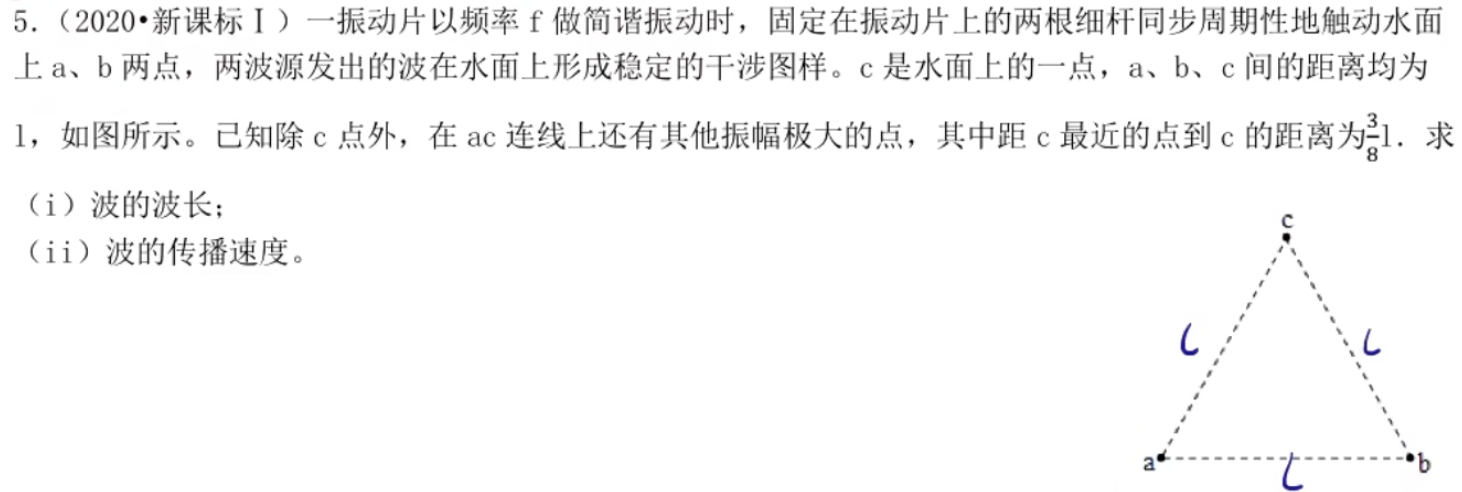
\includegraphics[width = 0.95\textwidth]{./pictures/2.1-4.png}

\begin{itemize}
    \item 正解:\quad $(1)\,\frac{1}{4}L \quad (2)\,\frac{1}{4}fL$
    \item 总结:\quad 需要理清波源为哪两个点,同时找到某个振动加强点(多少个$\lambda$)到波源的两个距离,余弦定理做计算.
    \item 扩展:\quad 三角函数相关
          \begin{formal}
              \begin{itemize}
                  \item 展开
                        $$ \sin{(\theta \pm \beta)} = \sin{\theta}\cos{\theta} \pm \cos{\theta}\sin{\theta} $$
                        $$ \cos{(\theta \pm \beta)} = \cos{\theta}\cos{\theta} \mp \sin{\theta}\sin{\theta} $$
                        $$ \tan{(\theta \pm \beta)} = \dfrac{\tan{\theta} \pm \tan{\beta}}{1 \mp \tan{\theta}\tan{\beta}}$$

                  \item 余补关系
                        $$ \sin{(\pi - \theta)} = \sin{\theta} \quad \cos{(\pi - \theta)} = - \cos{\theta} \quad \tan{(\pi - \theta)} = -\tan{\theta}$$

                        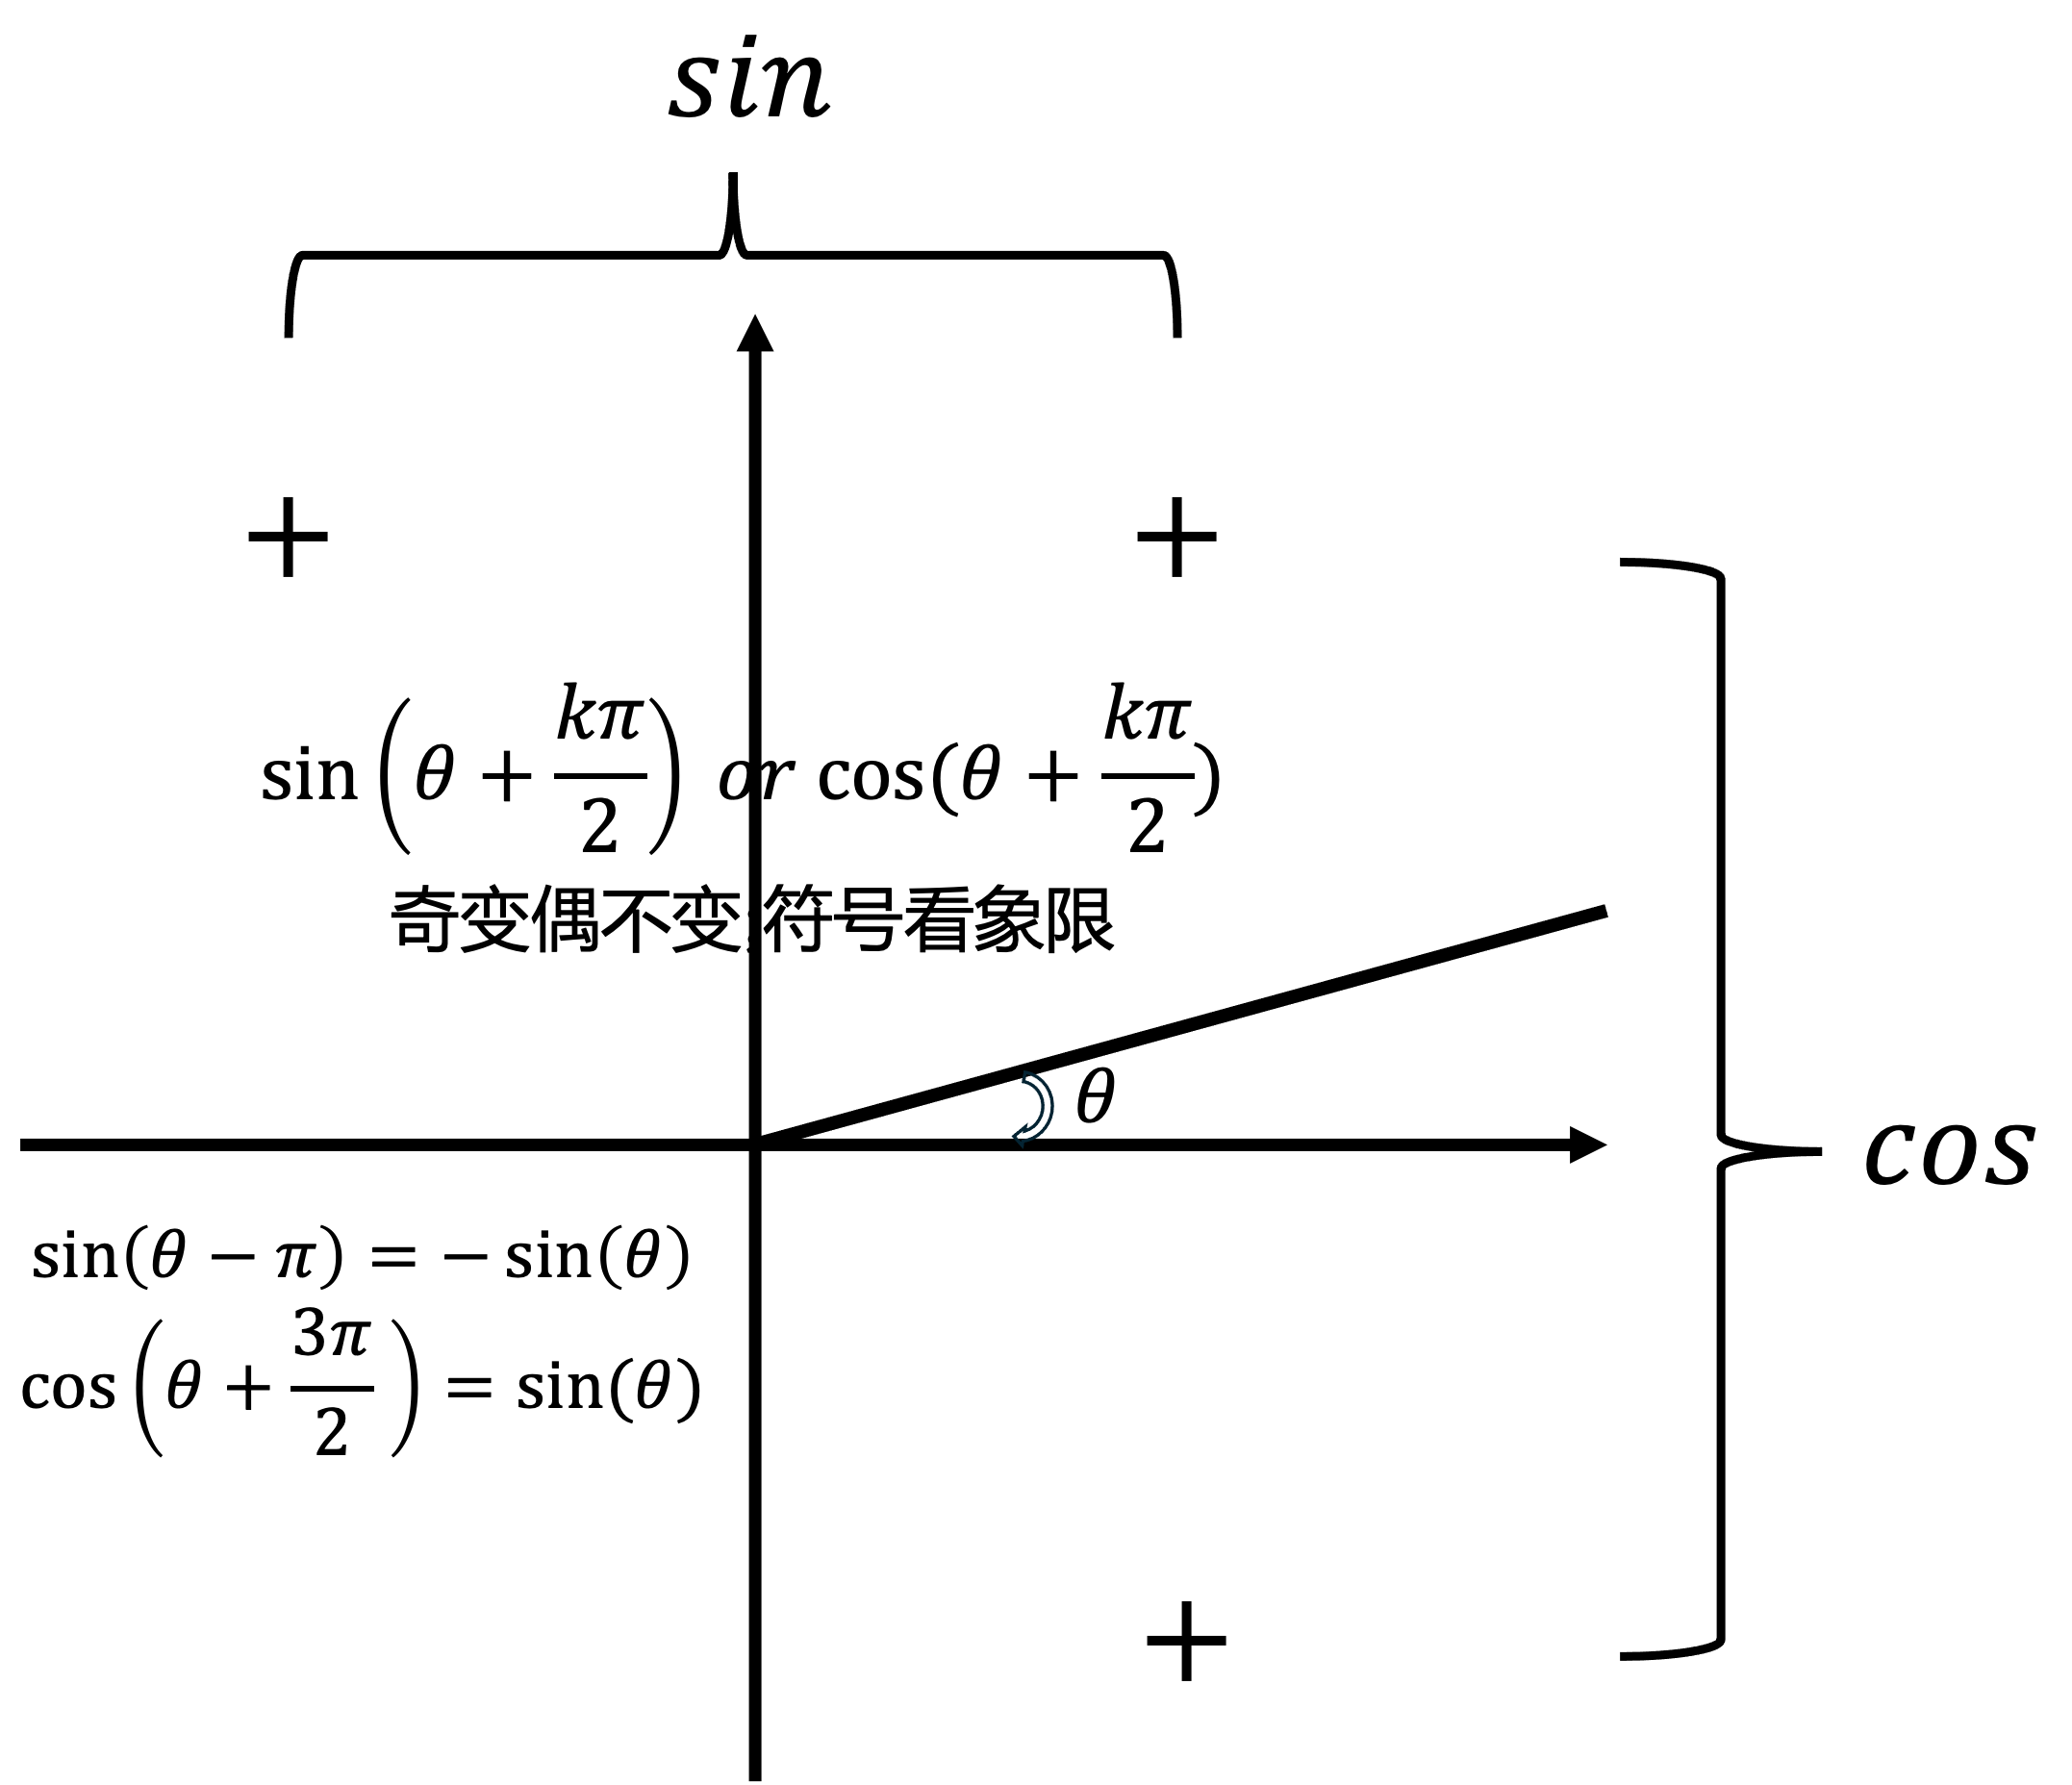
\includegraphics[width = 20em]{./pictures/2.1-5.png}

                  \item 正弦定理
                        $$ \dfrac{a}{\sin{\alpha}} = \dfrac{b}{\sin{\beta}} = \dfrac{c}{\sin{\gamma}}   $$

                  \item 余弦定理
                        $$ \cos{\gamma} = \dfrac{a^{2}+b^{2} - c^{2}}{2ab} $$

                  \item 二倍角
                        $$ \sin{2\theta} = 2\sin{\theta}\cos{\theta} \quad \cos{2\theta} = \cos^{2}{\theta} - \sin^{2}{\theta} \quad \tan{2\theta} = \dfrac{2\tan{\theta}}{1-\tan^{2}{\theta}}$$

                  \item 降次
                        $$ \sin^{2}{\theta} = \dfrac{1 - \cos{2\theta}}{2} \quad \cos^{2}{\theta} = \dfrac{1 + \cos{2\theta}}{2} \quad \tan^{2}{\theta} = \dfrac{1-\cos{2\theta}}{1+\cos{2\theta}}$$
              \end{itemize}
          \end{formal}
\end{itemize}

\vspace{2em}

\subsection{原子核物理}
\subsubsection{I-1: 不同原子核的平均值质量和}
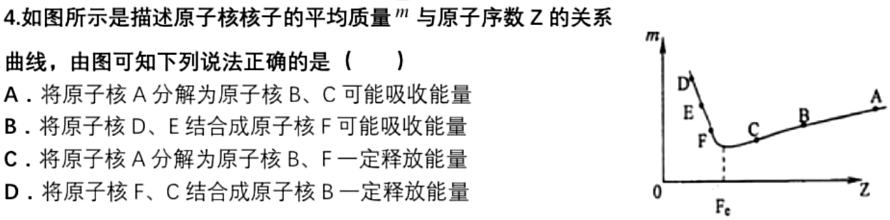
\includegraphics[width = 0.95\textwidth,keepaspectratio]{./pictures/2.2-1.png}

\begin{itemize}
    \item 正解:\quad $C$
    \item 总结:\quad 质量亏损释放能量,质量增大吸收能量

          \hspace{3.3em}在计算某两种元素原子核的平均质量时,并不是简单的加和

          \hspace{3.3em}例如$B \, C$两种元素混合后其平均质量值应该介于两者之间.
\end{itemize}

\vspace{2em}

\subsubsection{II-1: 比结合能大小与能量吸收释放}
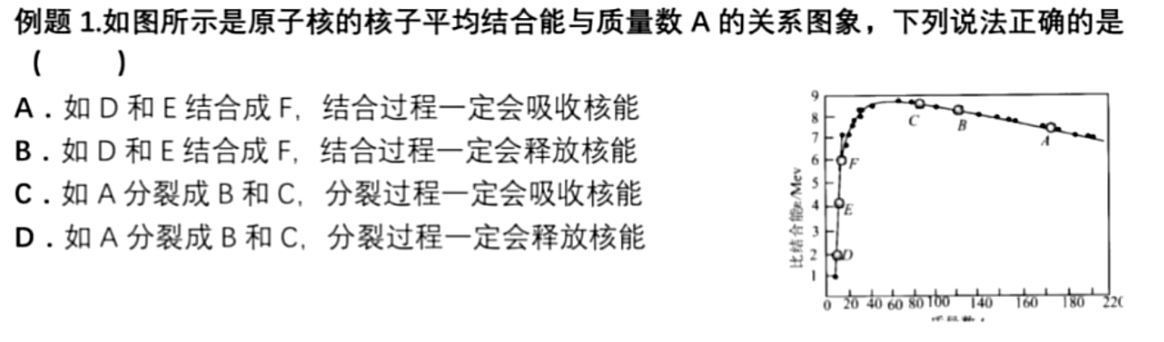
\includegraphics[width = 0.95\textwidth,keepaspectratio]{./pictures/2.2-2.png}

\begin{itemize}
    \item 正解:\quad $BD$
    \item 总结:\quad 比结合能越大则原子核状态更稳定,具备更低的能量状态.因此当比结合能上升时释放能量

          \hspace{3.3em}多元素的比结合能的计算类同理与平均质量
\end{itemize}

\subsection{热学}
\subsubsection{I-1: 三管连通器}
已知$h_{1};h_{2};h_{3};P_{A}$,求解$P_{B}$

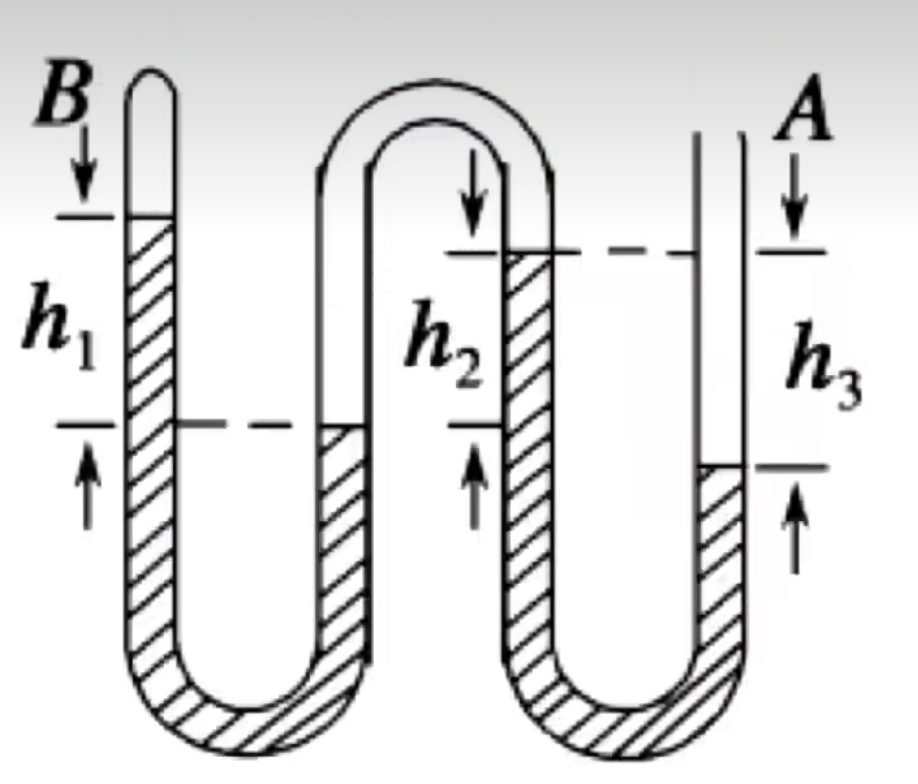
\includegraphics[width = 0.3\textwidth,keepaspectratio]{./pictures/2.3-1.png}
\begin{itemize}
    \item 正解:\quad $P_{B} = P_{A} + \rho g (h_{3} - h_{1}) $
    \item 总结:\quad 前两管: $ P_{B} + \rho g h_{1} = P_{C}\text{,后两管} P_{C} + \rho g h_{3} = P_{0}$

\end{itemize}

\vspace{2em}

\subsubsection{I-2: 液泡上浮问题}
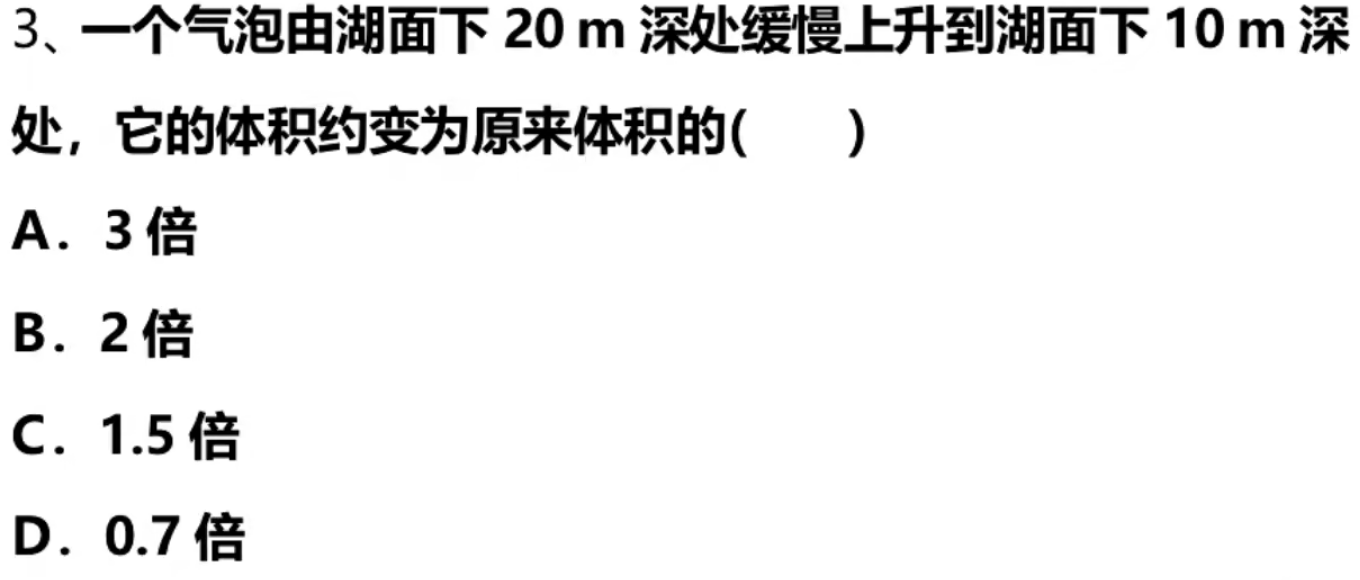
\includegraphics[width = 0.55\textwidth,keepaspectratio]{./pictures/2.3-2.png}

\begin{itemize}
    \item 正解:\quad $C$
    \item 总结:\quad 外界大气压的作用应该被计算进去
\end{itemize}

\vspace{2em}

\subsubsection{I-3: 图像计算}
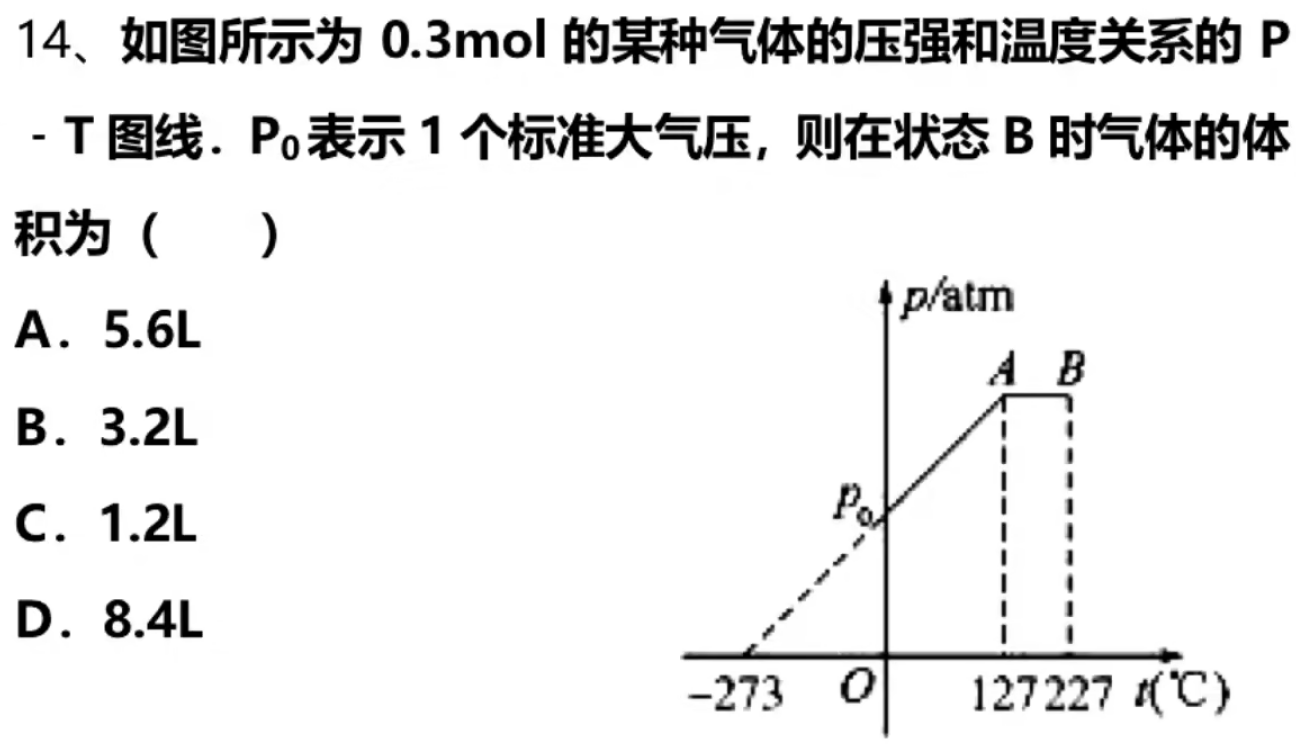
\includegraphics[width = 0.55\textwidth,keepaspectratio]{./pictures/2.3-3.png}

\begin{itemize}
    \item 正解:\quad $D$
    \item 总结:\quad 首先应该向左平移$y$轴,使得横坐标换算成开尔文温度.

          \hspace{3.3em}新的坐标系下,斜线$OA$满足$P = \frac{C}{V}T$斜率为定值,因此为等容过程.

          \hspace{3.3em}$T = 273k$时直线过$P_{0}$,此时气体体积为$22.4L$,因此$V_{A} = 22.4L$
          
          \hspace{3.3em}横线$A \ra B$为等压过程,计算温度之比即可求得$V_{B}$
\end{itemize}

\vspace{2em}

\subsubsection{I-4: 液柱动力学问题}
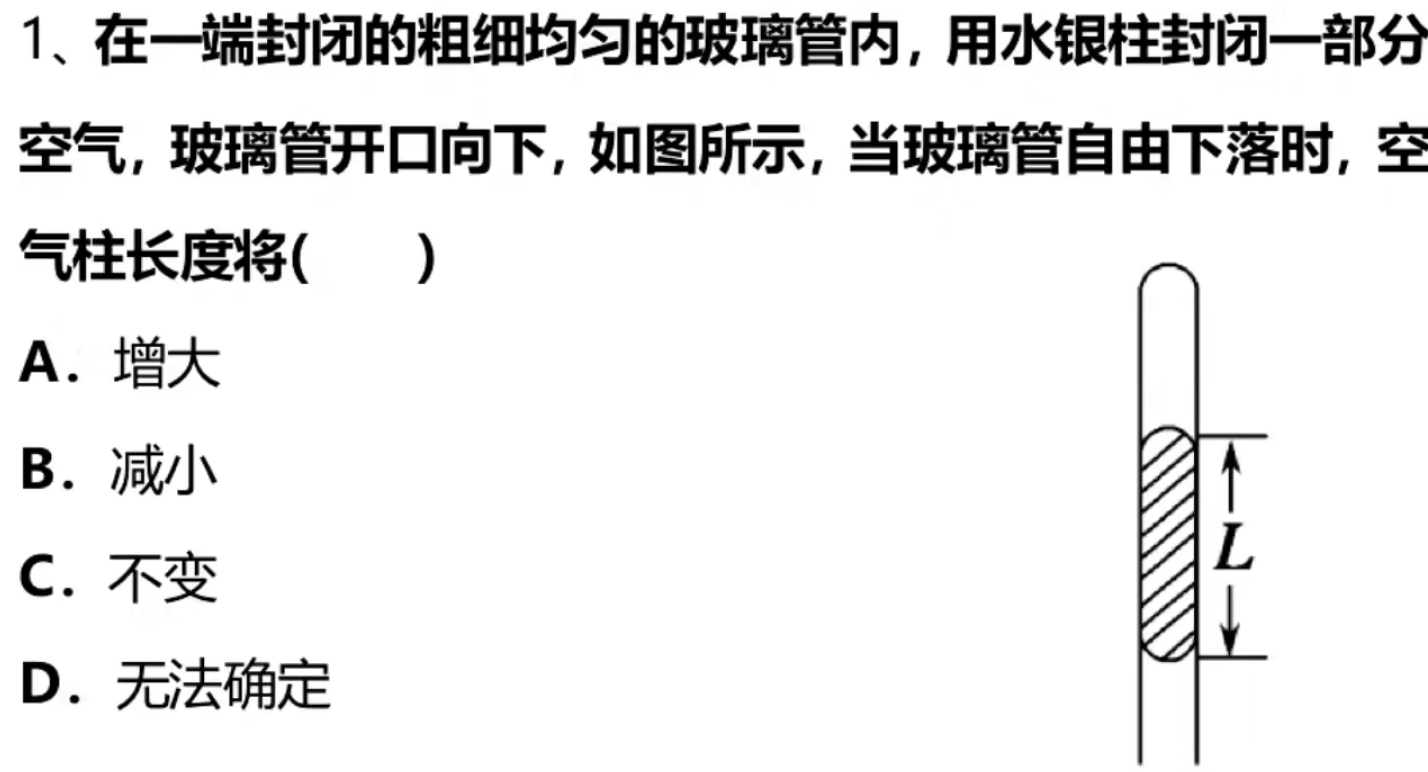
\includegraphics[width = 0.55\textwidth,keepaspectratio]{./pictures/2.3-4.png}

\begin{itemize}
    \item 正解:\quad $B$
    \item 总结:\quad 动力学问题主要在于分析好初末态,同时列受力分析方程.

          \hspace{3.3em}初态$PS + mg = P_{0}S$,末态自由落体加速度为$g$

          \hspace{3.3em}$P^{'}S + mg - P_{0}S = ma = mg \lra P^{'} = P_{0}$液柱上方压强增大,因此液柱上方体积减小
\end{itemize}

\vspace{2em}

\subsubsection{I-5: 等体两气挤压问题}
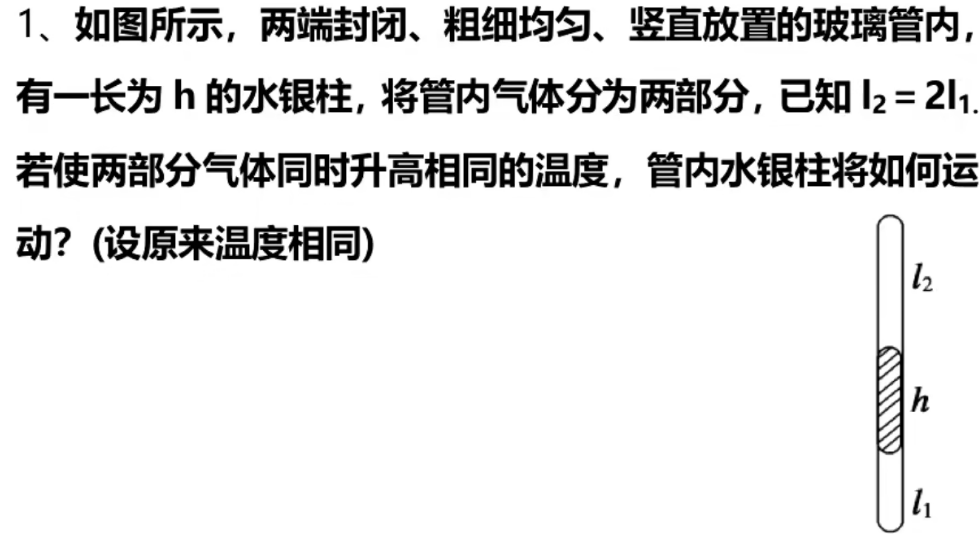
\includegraphics[width = 0.55\textwidth,keepaspectratio]{./pictures/2.3-5.png}

\begin{itemize}
    \item 正解:\quad 向上移动
    \item 总结:\quad 三个状态参量中,真正使得液柱移动的物理量是$P$,在查理定律中$\frac{P}{T} = \frac{C}{V}$

          \hspace{3.3em}升温瞬间可视为\textbf{等体}过程,因此函数为过原点的直线可得$\frac{P}{T} = \frac{\triangle P}{\triangle T}$

          \hspace{3.3em}$ \triangle P_{1} = \frac{P_{1}}{T_{1}} \triangle T = \frac{C}{V_{1}} \triangle T $

          \hspace{3.3em}$ V_{2} = 2 V_{1}  \quad \lra \triangle P_{1} > \triangle P_{2}$
\end{itemize}

\vspace{2em}

\subsubsection{I-5: 斜试管等体变化液面移动与稳态分析}
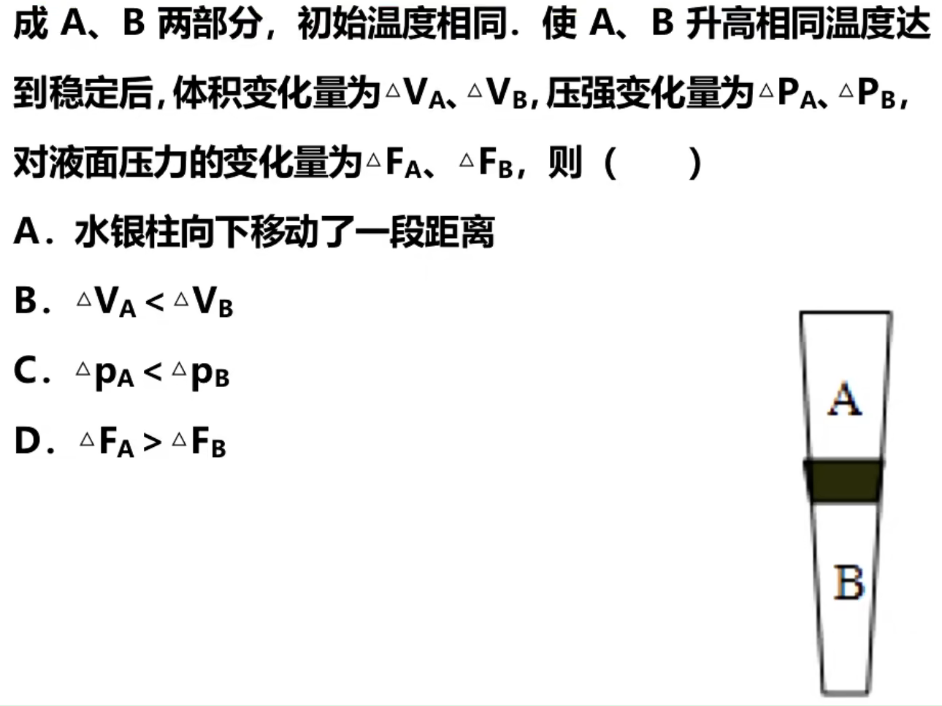
\includegraphics[width = 0.55\textwidth,keepaspectratio]{./pictures/2.3-6.png}


\begin{itemize}
    \item 正解:\quad $D$
    \item 总结:\quad (此题有时候瞬态与稳态的$\triangle$是混用的,变化量与变化量绝对值$\triangle$也是混用的)

          \hspace{2.5em}\begin{minipage}{0.88\textwidth}
              \begin{enumerate}[label = (\arabic*)]
                  \item 判断移动使用瞬态公式(这里的$\triangle$表示的瞬态并非题干中的稳态)
                        \begin{align*}
                             & \triangle P_{A} = \frac{P_{A}}{T} \triangle T  \quad  \triangle P_{B} = \frac{P_{B}}{T} \triangle T \\
                             & P_{B} > P_{A} \lra \triangle P_{B} > \triangle P_{A} \quad \text{液柱向上移动}                            \\
                             & \text{向上移动的过程中,液面上下表面的面积也在发生改变,液体的高度因为面积的增大而减小}
                        \end{align*}
                  \item 由于整个管内是封闭的,且认为液体的体积是不会改变的,因此$\triangle V_{A} = \triangle V_{B}$
                  \item $P_{A}^{'} + h^{'} = P_{B}^{'} \quad h^{'} \text{是由}h\text{变小} \, \triangle h < 0 \lra \triangle P_{A} > \triangle P_{B} $
                  \item 需要列受力分析方程$ F_{A}^{'} + F_{\text{斜}} + mg = F_{B}^{'}$

                        由于液面的上升,液面高度下降了,压在侧面的液体体积减少,因此$\triangle F_{\text{斜}} < 0 \lra \triangle F_{A} > \triangle F_{B}$
              \end{enumerate}
          \end{minipage}
\end{itemize}

\vspace{2em}

\subsubsection{I-6: 等压液面移动问题}
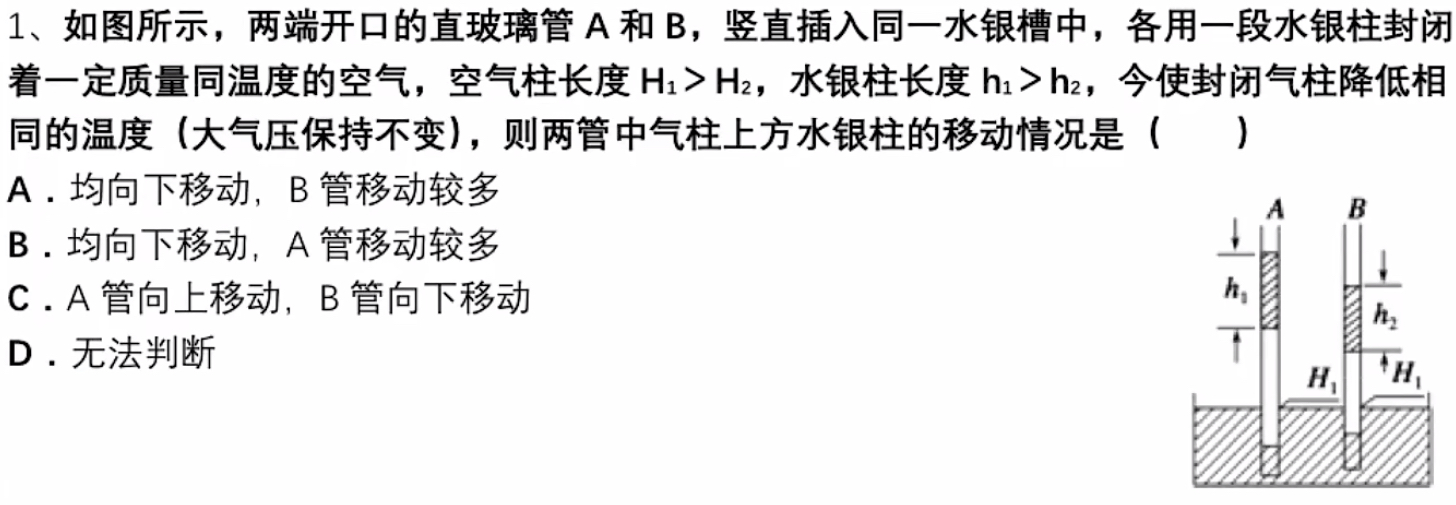
\includegraphics[width = 0.95\textwidth,keepaspectratio]{./pictures/2.3-7.png}

\begin{itemize}
    \item 正解:\quad $B$
    \item 总结:\quad

          \hspace{3em}\begin{minipage}{0.88\textwidth}
              此题不能使用等体过程的$\frac{\triangle P}{\triangle T}$进行分析

              两试管各自独立,区别于等体两气挤压问题(作用对象为同一个液柱)

              但两试管均连通大气$P_{0} + h_{1} = P_{A} \quad P_{0} + h_{2} = P_{B}$

              因此可视作等压过程,同有过原点的直线$V = \frac{1}{P} T \lra \frac{V}{T} = \frac{\triangle V}{\triangle T}$

              $V_{A} = \frac{\triangle V_{A}}{\triangle T} T \quad V_{A} > V_{B} (\text{两者均为负数,液柱下移})\lra \triangle V_{A} > \triangle V_{B}$
          \end{minipage}
\end{itemize}

\vspace{2em}

\subsubsection{I-7: 试管移动问题}
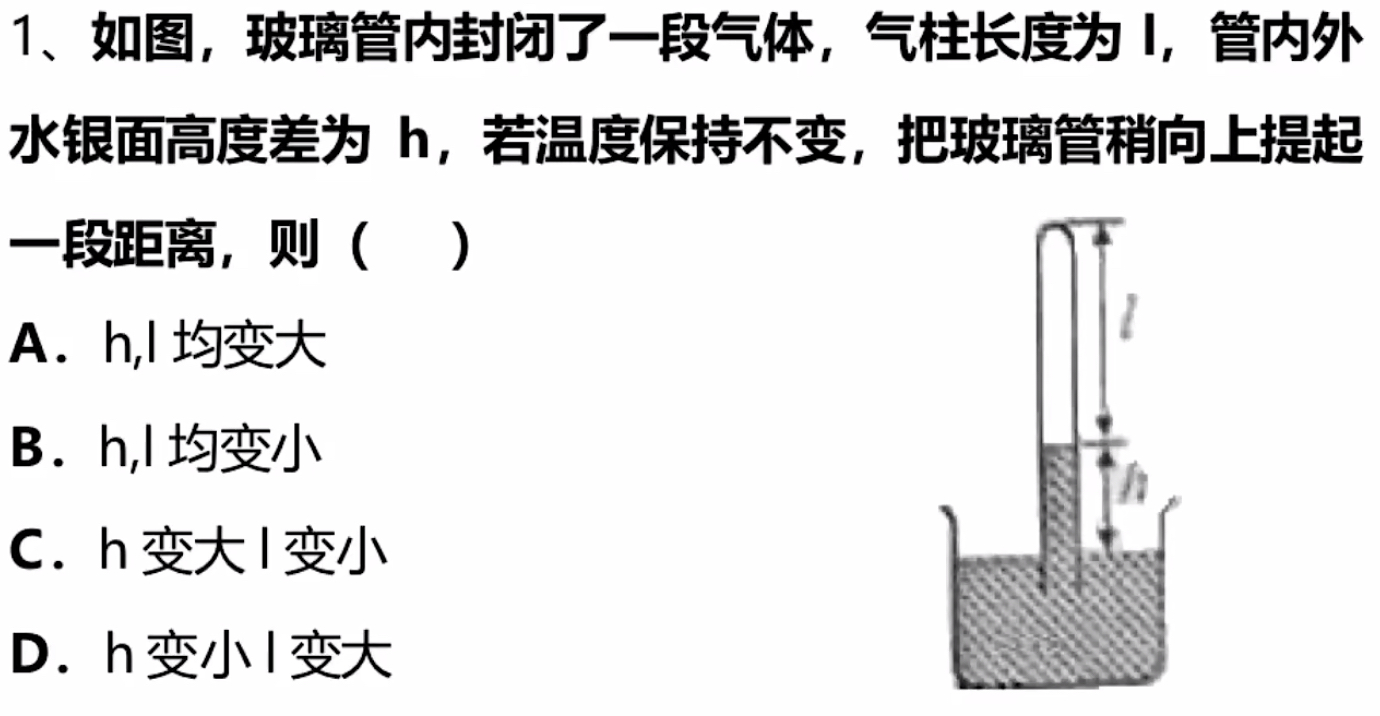
\includegraphics[width = 0.55\textwidth,keepaspectratio]{./pictures/2.3-8.png}

\begin{itemize}
    \item 正解:\quad $A$
    \item 总结:\quad

          \hspace{3em}\begin{minipage}{0.88\textwidth}
              此题没有明确的等状态参量(有等温条件但是在此题中没有直接作用)

              可以视作\text{等体}(气体体积不变)过程分析,即先假设$l$不变.

              初状态$P + h = P_{0}$,向上提试管,等体过程气体体积不变意味$l$不变,$h$变大,所以$P$减小

              $P$在等温过程中意味着$V$增大,压缩液柱$h$减小.

              $h$在此分析过程中既有增大也有减小.很难直接分析哪个改变量更大

              只需分析末状态$P + h = P_{0}$,$P$是一定在减小的,因此末状态$h$是增大的.所以$h \, l$均增大
          \end{minipage}
\end{itemize}

\subsubsection{I-8: 液面移动综合分析 }
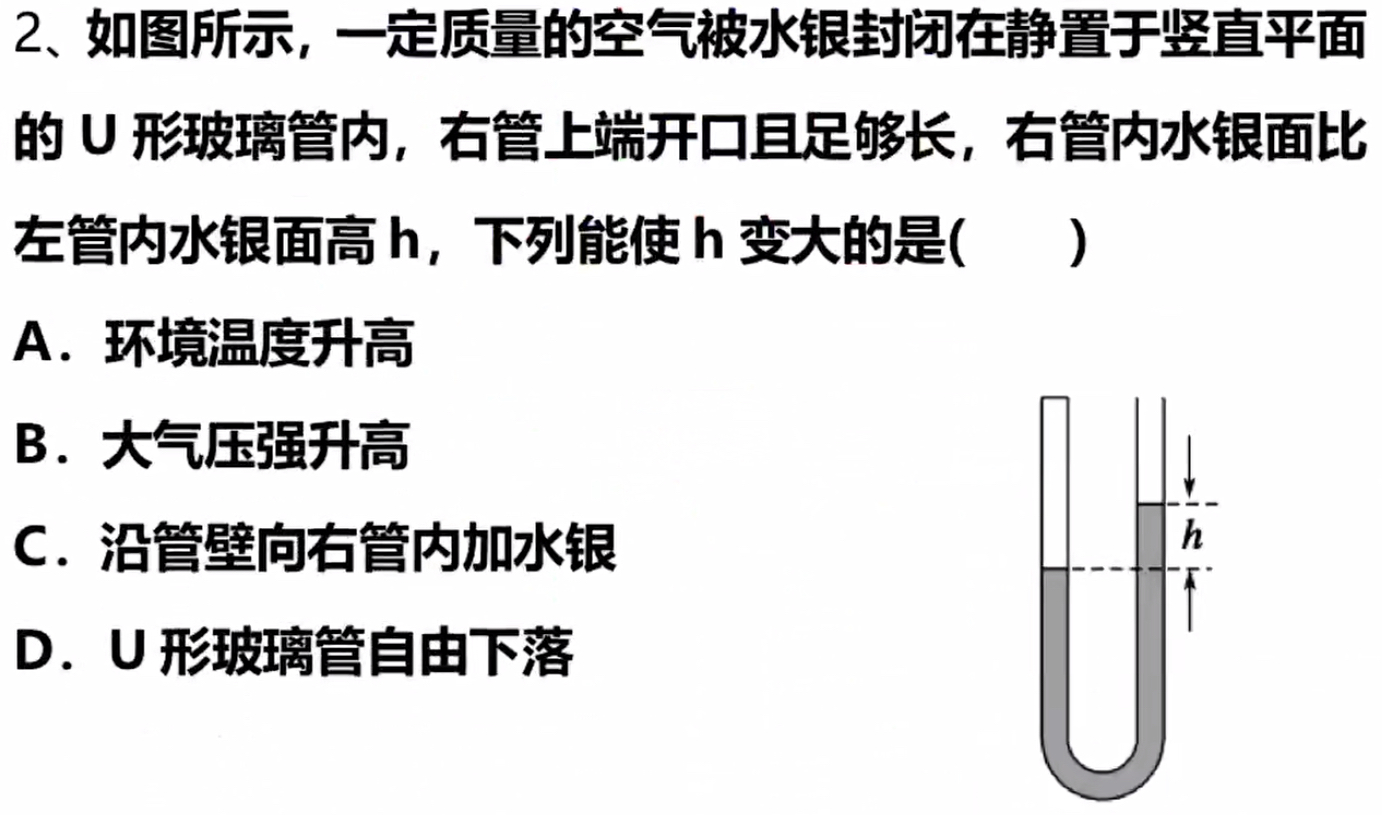
\includegraphics[width = 0.55\textwidth,keepaspectratio]{./pictures/2.3-9.png}

\begin{itemize}
    \item 正解:\quad $ACD$
    \item 总结:\quad

          \hspace{3em}\begin{minipage}{0.88\textwidth}
              \begin{enumerate}[label = (\Alph*)]
                  \item 通常当多个变量发生变化,优先假设$V$不变,因此瞬态满足$\frac{P}{T} = \frac{\triangle P}{\triangle T} = C$

                        $P = P_{0} + h$方程右边暂时不变,环境温度上升$\triangle T > 0 \lra \triangle P > 0$,压强$P$增大

                        虽然体积$V$减小导致$h$又下降,但稳态总有$P$变大,因此需要$h$变大,$A$正确
                  \item $P_{0}$上升,$P$上升,等温条件下$V$下降,因此试管左边的体积下降导致$h$变小
                  \item 可以从两个角度思考,只要持续往里加水银,必然会使得液面高$h$上升

                        另一个角度,瞬态时$h$变大,$P$变大,$V$减小,末态方程$P^{'} = P_{0} + h^{'}$

                        结果上必然有$P^{'}>P$,因此$h$变大
                  \item 自由落体需要列动力学方程,$P_{0}S + mg - P^{'}S = mg \lra P^{'} = P_{0}$压强变小,体积变大,$h$上升
              \end{enumerate}
          \end{minipage}
\end{itemize}

\vspace{2em}

\subsubsection{I-9: 充气问题}
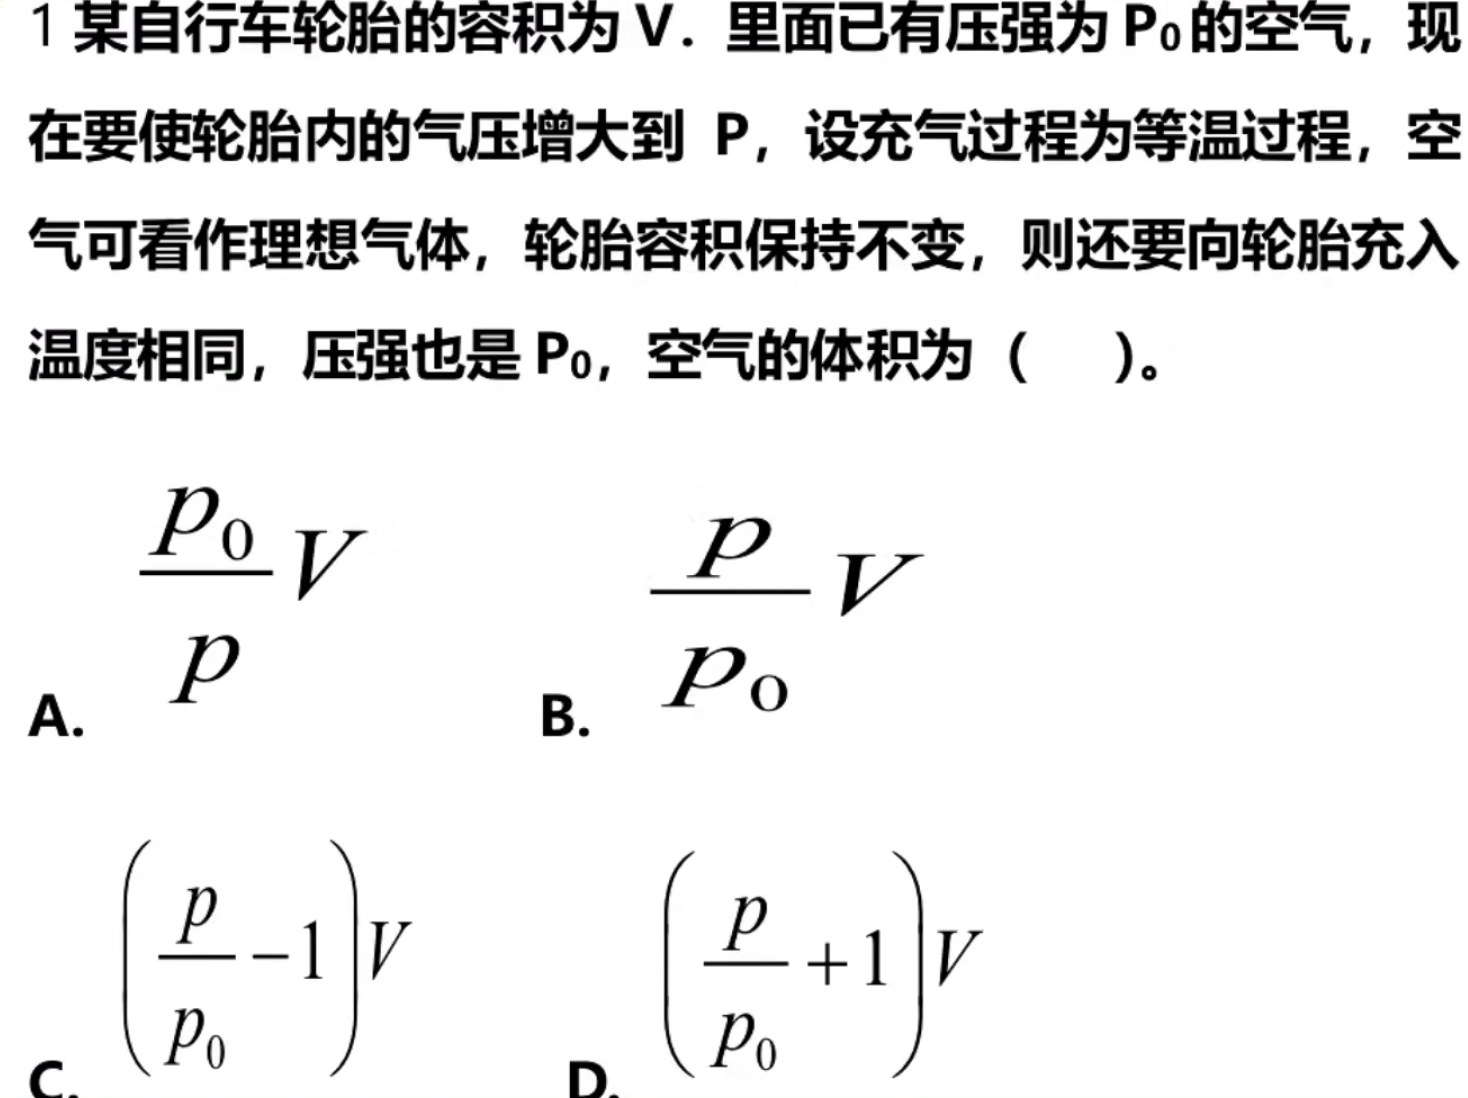
\includegraphics[width = 0.55\textwidth,keepaspectratio]{./pictures/2.3-10.png}

\begin{itemize}
    \item 正解:\quad $C$
    \item 总结:\quad

          \hspace{3.2em}\begin{minipage}{0.88\textwidth}
              \begin{align*}
                                        & \text{由于是限容问题,本质上是求}:\triangle n \llra \triangle V                                          \\
                  P_{0}V                & = n_{1}RT                                                                                   \\
                  PV                    & = n_{2}RT \quad \lra \quad (P-P_{0})V = (n_{2} - n_{1})RT                                   \\
                  P_{0} \triangle V     & = \triangle n RT = (n_{2} - n_{1})RT  \quad \lra \quad \triangle V = (\frac{P}{P_{0}} - 1)V \\
                                        & \text{或者使用一个方程要求: 原状态 \, + \, 打入气 = 末状态}                                                    \\
                  P_{0} V + P_{0} V_{0} & = PV \quad \lra \quad \triangle V = (\frac{P}{P_{0}} - 1)V
              \end{align*}
          \end{minipage}

\end{itemize}

\vspace{2em}

\subsubsection{I-10: 物理现象中的热力学定律问题}
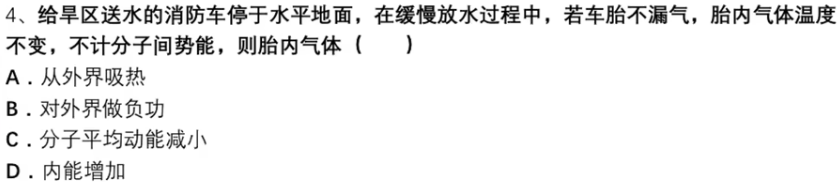
\includegraphics[width = 0.95\textwidth,keepaspectratio]{./pictures/2.3-32.png}

\begin{itemize}
    \item 正解:\quad $A$
    \item 总结:\quad 重点在于洒水车在洒水的过程中,对轮胎的压力在下降
    
    \hspace{2.7em} 因此轮胎内的气体是在膨胀的,气体对外做功$W < 0$,温度不变因此$\triangle u = 0 \lra Q > 0$
\end{itemize}

\vspace{2em}

\subsubsection{I-11: 热力学定律的图像问题1}
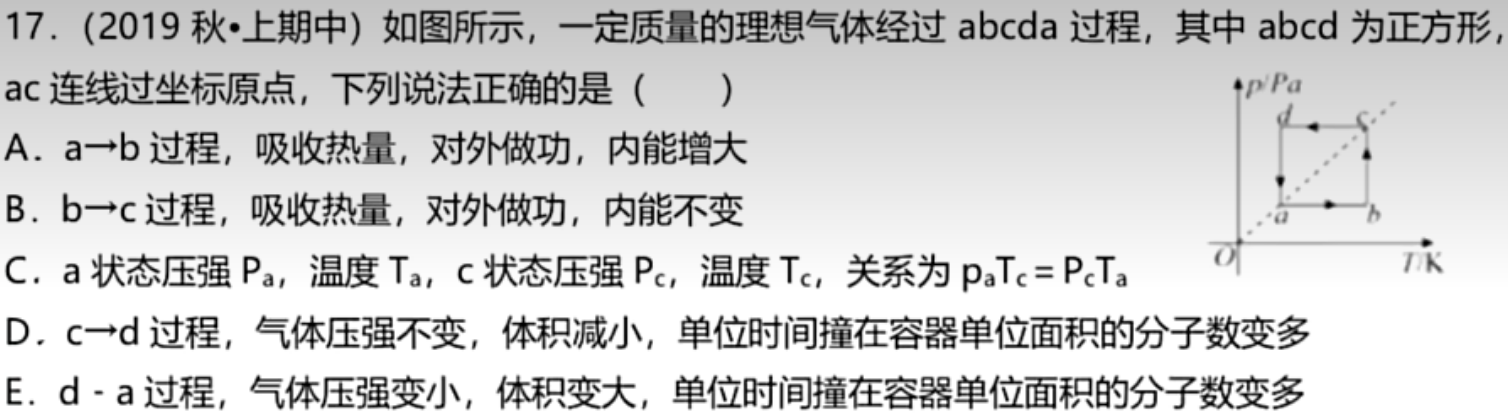
\includegraphics[width = 0.95\textwidth,keepaspectratio]{./pictures/2.3-33.png}

\begin{itemize}
    \item 正解:\quad $ACD$
    \item 总结:\quad $D \, E$选项的判断体积越小,那么显然单位体积内的分子数上升,碰撞容器壁的概率会上升
\end{itemize}

\vspace{2em}

\subsubsection{I-12: 热力学定律的图像问题2}
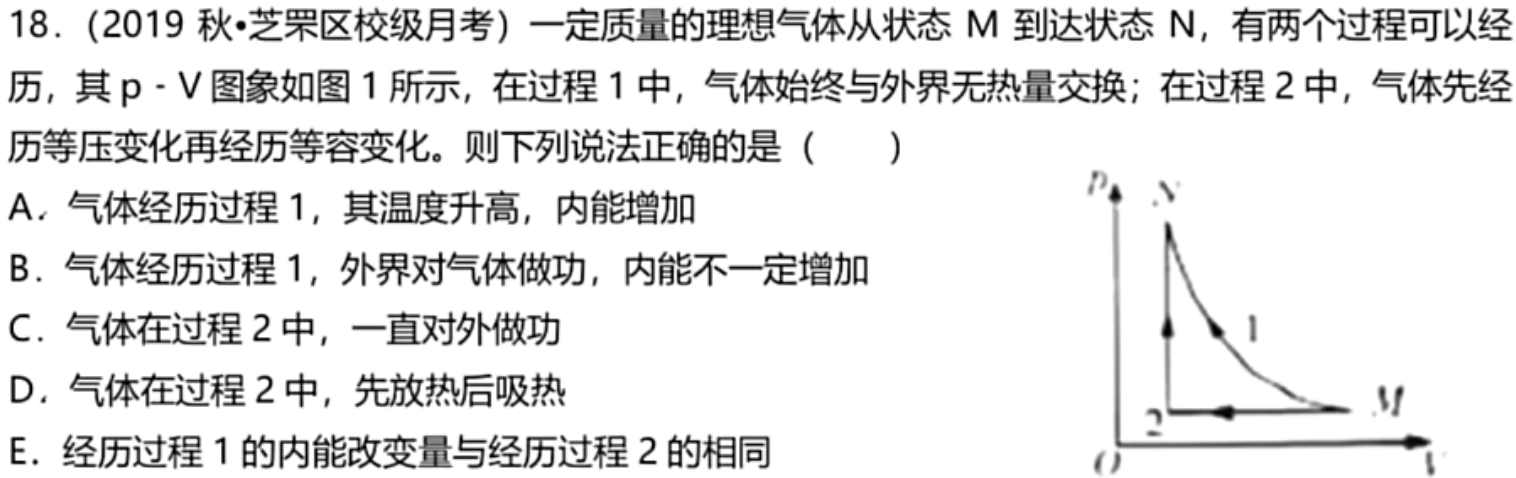
\includegraphics[width = 0.95\textwidth,keepaspectratio]{./pictures/2.3-34.png}

\begin{itemize}
    \item 正解:\quad $ADE$
    \item 总结:\quad $E$选项由于是理想气体,因而温度的改变量决定内能的改变量
    
    \hspace{2.7em}初末状态一致,因此实际温度的改变量也一样,所以内能的改变量一样
\end{itemize}

\vspace{2em}

\subsubsection{I-13: 热力学定律的图像问题3}
\includegraphics[width = 0.95\textwidth,keepaspectratio]{./pictures/2.3-35.png}

\begin{itemize}
    \item 正解:\quad $BCE$
\end{itemize}

\vspace{2em}

\subsubsection{I-14: 热力学定律的图像问题4}
\includegraphics[width = 0.95\textwidth,keepaspectratio]{./pictures/2.3-36.png}

\begin{itemize}
    \item 正解:\quad $BCD$
    \item 总结:\quad $E$选项注意能量的转化角度,热量一部分转化为对外做功一部分作为内能储存
\end{itemize}

\vspace{2em}

\subsubsection{I-15: 热力学定律的图像问题5}
\includegraphics[width = 0.95\textwidth,keepaspectratio]{./pictures/2.3-37.png}

\begin{itemize}
    \item 正解:\quad $BDE$
\end{itemize}

\vspace{2em}

\subsubsection{I-16: 热力学定律的图像问题6}
\includegraphics[width = 0.95\textwidth,keepaspectratio]{./pictures/2.3-38.png}

\begin{itemize}
    \item 正解:\quad $ABD$
\end{itemize}

\vspace{2em}

\subsubsection{IV-1: 放气问题}
\includegraphics[width = 0.55\textwidth,keepaspectratio]{./pictures/2.3-11.png}

\begin{itemize}
    \item 正解:\quad $25$次
    \item 总结:\quad 主要在于排出气体的压强与水压+大气压平衡,是恒压为$1 \, atm + P_{\text{水}}$,其中$P_{\text{水}} = 15 \, atm$
\end{itemize}

\vspace{2em}

\subsubsection{IV-1: 单试管加液问题}
\includegraphics[width = 0.95\textwidth,keepaspectratio]{./pictures/2.3-12.png}

\begin{itemize}
    \item 正解:\quad $(1) \, 450k$  $(2) \, 7cm$
    \item 总结:\quad $(1)$问中转化为开尔文温度计算;$(2)$问假设加入了$x \, cm$水银柱来分析末状态.计算量较大
\end{itemize}

\vspace{2em}

\subsubsection{IV-2: 单试管液柱加速问题}
\includegraphics[width = 0.95\textwidth,keepaspectratio]{./pictures/2.3-13.png}

\begin{itemize}
    \item 正解:\quad $(1) \, \frac{1}{2}l$  $(2) \, \frac{P_{0}S + mg}{P_{0}S + ma} l$
    \item 总结:\quad $(2)$问在于水平放置的刚开始左端气压为初始竖直状态下的气压,稳定时液柱向右以加速度$a$运动

          \hspace{3.2em}$PS - P_{0}S = ma \quad$ (水平后液柱重力竖直向下,对分析过程并不产生作用)
\end{itemize}

\vspace{2em}

\subsubsection{IV-3: 单试管多过程问题}
\includegraphics[width = 0.95\textwidth,keepaspectratio]{./pictures/2.3-14.png}

\begin{itemize}
    \item 正解:\quad $(1) \, \frac{1}{2}T_{1}$  $(2) \, 0.75P_{0}$
    \item 总结:\quad 多过程问题重点在于分清楚每个阶段满足的平衡方程与物态方程
\end{itemize}

\vspace{2em}

\subsubsection{IV-4: 单试管多过程问题2}
\includegraphics[width = 0.95\textwidth,keepaspectratio]{./pictures/2.3-15.png}

\begin{itemize}
    \item 正解:\quad $(1) \, \frac{1}{3}h$  $(2) \, 3T_{0}$
\end{itemize}

\vspace{2em}

\subsubsection{IV-5: 气缸多过程问题}
\includegraphics[width = 0.95\textwidth,keepaspectratio]{./pictures/2.3-16.png}

\begin{itemize}
    \item 正解:\quad $(1) \, 4 \, kg$  $(2) \, 640 \, cm^{3}$
    \item 总结:\quad $(1)$问求解活塞质量其实为分析一个等体升温过程;$(2)$可以假设固体体积$V_{0}$进行计算即可
\end{itemize}

\vspace{2em}

\subsubsection{IV-6: L型试管分类讨论问题}
\includegraphics[width = 0.95\textwidth,keepaspectratio]{./pictures/2.3-17.png}

\begin{itemize}
    \item 正解:\quad $(1) \, 24 \, cm$  $(2) \, 23.5 \, cm $
    \item 总结:\quad $(1)$问注意在分析平衡方程时,水平的液柱并不产生作用,只需要竖直部分

          \hspace{3.2em}$(2)$问应当注意的时需要分析液柱是否被完全挤压出竖直部分,当为完全挤压时$P = P_{0}$

          \hspace{3.2em}具体分析方法为假设刚好完全挤压出去,得到此时所需要的压强$P_{x}$,比较和刚竖直时的压强

          \hspace{3.2em}若$P_{x}$较小则将继续挤压,那么$P = P_{0}$.否则只挤出一部分,竖直方向仍有水银柱
\end{itemize}

\vspace{2em}

\subsubsection{IV-7: L型试管分类讨论问题2}
\includegraphics[width = 0.95\textwidth,keepaspectratio]{./pictures/2.3-18.png}

\begin{itemize}
    \item 正解:\quad $(1) \, 516 \, k$  $(2) \, 52.6 \, cm $
    \item 总结:\quad $(2)$问的特殊点就在于,液柱完全被挤压出竖直方向($P_{x} = 80 \, cmHg < 96 \, cmHg$)

          \hspace{3.2em}所以被封空气柱的压强应当$76 \, cmHg$计算
\end{itemize}

\vspace{2em}

\subsubsection{IV-8: 挤压液体临界情况分析}
如图所示,一竖直放置且开口向上的玻璃管,长度为$L = 94 \, cm$,管里一段长为$h = 24 \, cm$的水银柱封闭

一段理想气体,气体的长度为$l = 50 \, cm$,环境温度为$27 ^{\circ} C$,大气压强为$76 \, cmHg$,求:

$(1)$当水银柱恰好上升到玻璃管顶部,此时气体温度为多少?

$(2)$要使水银全部溢出,则气体温度为多少?

\vspace{1em}

\begin{minipage}{0.4\textwidth}
    \includegraphics[width = 0.16\textwidth,keepaspectratio]{./pictures/2.3-19.png}
\end{minipage}
\hfill
\begin{minipage}{0.5\textwidth}
    \includegraphics[width = 0.8\textwidth,keepaspectratio]{./pictures/2.3-20.png}
\end{minipage}


\begin{itemize}
    \item 正解:\quad $(1) \, 420 \, k$  $(2) \, 433.5 \, k $
    \item 总结:\quad $(2)$问的临界情况比较特殊,液体是连续不断的被挤压出试管

          \hspace{3.2em}所以在此过程中液体的质量在不断减少,所需要的压强也变少了

          \hspace{3.2em}所以达到某个临界温度时,停止升温,依靠自身的压强可以完成后续的挤压过程

          \hspace{3.2em}因此需要假设所剩液柱高度为$x \, cm$时,后续依靠自身压强

          \hspace{3.2em}$\frac{100 \, S \, 50 }{300} = \frac{(76+x)(94-x) \, S}{T} \quad \lra \quad T = \frac{3}{50} (76+x)(94-x)$

          \hspace{3.2em}该函数在$x \in [0,24] $区间上的图像如右上所示.物理过程$x$逐渐减小(函数从右向左看).

          \hspace{3.2em}$x$从大变小的过程中,需要的温度逐渐上升.

          \hspace{3.2em}在此区间抛物线函数上,取到最大温度$T = 433.5k$后(对应$x=9cm$)

          \hspace{3.2em}则可靠当前压强继续挤压液体溢出.若是直接使用完全溢出后连通大气的压强计算

          \hspace{3.2em}得到的温度$T = 428.64 \, k$恰是越过了抛物线顶端向左的一个值

          \hspace{3.2em}所以符合物理实际过程的温度是顶端温度$433.5 \, k$

\end{itemize}

\vspace{2em}

\subsubsection{IV-9: 双气缸平衡问题}
\includegraphics[width = 0.95\textwidth,keepaspectratio]{./pictures/2.3-21.png}

\begin{itemize}
    \item 正解:\quad $(1) \, 4 \, T$  $(2) \, 5:4 $
    \item 总结:\quad 隐含的条件是,在平衡状态下活塞是无法移动的,因此两边气体的压强必然相等
\end{itemize}

\vspace{2em}

\subsubsection{IV-10: 双气缸平衡问题2}
\includegraphics[width = 0.95\textwidth,keepaspectratio]{./pictures/2.3-22.png}

\begin{itemize}
    \item 正解:\quad $(1) \, \frac{5}{3} \, P_{0}$  $(2) \, \frac{4}{3} T_{0} $
    \item 总结:\quad 此题的对于可导热气缸$A$而言,其温度始终与环境温度一致
    
    \hspace{3.2em} 注意活塞和气缸$B$是不导热的,所以打开阀门后$B$的温度发生变化
\end{itemize}

\vspace{2em}

\subsubsection{IV-11: 双活塞平衡问题}
\includegraphics[width = 0.95\textwidth,keepaspectratio]{./pictures/2.3-23.png}

\begin{itemize}
    \item 正解:\quad $a$活塞向上移动$\frac{1}{12} \, L \quad b$活塞向上移动$\frac{1}{4} \, L$
    \item 总结:\quad 此题注意活塞与大气相连,因此平衡态三气恒压为大气压.
    
    \hspace{3.2em}且求出$a$活塞向上移动$\frac{1}{12} \, L $后,在求$b$活塞时得出$\frac{2}{3} \, L \quad $变为$\frac{1}{2} \, L $ 

    \hspace{3.2em}活塞$B$实际的移动距离需要考虑活塞$a$的移动距离$ \frac{2}{3} \, L + \frac{1}{12} \, L - x = \frac{1}{2} \, L \quad \lra x = \frac{1}{4} \, L$
\end{itemize}

\vspace{2em}

\subsubsection{IV-12: 双活塞漏气问题}
\includegraphics[width = 0.95\textwidth,keepaspectratio]{./pictures/2.3-24.png}

\begin{itemize}
    \item 正解:\quad $\triangle L = \frac{V}{S}(2 - \frac{(P_{0} + \frac{3mg}{S})}{P_{0} + \frac{mg}{S}})$
    \item 总结:\quad 活塞$B$漏气会使得下方气体(气压更大)向上充气.但是整体的而言气体都在容器内
    
    \hspace{3.2em}所以本质此问题是一个充气问题,需要用到涉及物质的量的方程  
    
    \hspace{3.2em}$\frac{(P_{0} + \frac{mg}{S}) V}{T_{0}} + \frac{(P_{0} + \frac{2mg}{S}) V}{T_{0}} = \frac{(P_{0} + \frac{mg}{S}) V^{'}}{T_{0}}  
    \quad \lra V^{'} = \frac{(P_{0} + \frac{3mg}{S})}{P_{0} + \frac{mg}{S}}$
\end{itemize}

\vspace{2em}

\subsubsection{IV-13: U型管问题}
\includegraphics[width = 0.95\textwidth,keepaspectratio]{./pictures/2.3-25.png}

\begin{itemize}
    \item 正解:\quad $(1) \, P_{1} = P_{0} + \frac{mg}{S} \quad (2) \, T_{1} = (1 + \frac{mg}{P_{0}S}) T_{0} \quad (3) \, T^{'} 
    = (1 + \frac{mg}{P_{0}S} + \frac{\rho g L}{P_{0}}) T_{0}$
    \item 总结:\quad 主要在于液面高度差$L$,在实际分析左侧试管下降高度为$\frac{1}{2}L$
\end{itemize}

\vspace{2em}

\subsubsection{IV-14: U型管移动问题}
\includegraphics[width = 0.95\textwidth,keepaspectratio]{./pictures/2.3-26.png}

\begin{itemize}
    \item 正解:\quad $(1) \, 8 \, cm \quad (2) \, 270 \, k$
    \item 总结:\quad $(1)$问容易得到错误答案$6 \, cm$,通过计算两管新的液柱高度差为$4 \, cm$,需要分步分析
    
    \hspace{3.2em}由于$A$管液面上升了$2 \, cm$,即先向上移动试管$2 \, cm$,此时右侧液面低于左侧$2 \, cm$

    \hspace{3.2em}再抬升$B$管直到右侧高于左侧$4 \, cm$,则需要抬升$8 \, cm$

    \hspace{3.2em}$(2)$问由于液面高度差为$4 \, cm $,$A$管气柱此时$38 \, cm$需要上升$2 \,cm$到$36 \, cm$计算
\end{itemize}

\vspace{2em}

\subsubsection{IV-15: 不同粗细U型管的活塞移动问题}
\includegraphics[width = 0.95\textwidth,keepaspectratio]{./pictures/2.3-27.png}

\begin{itemize}
    \item 正解:\quad $(1) \, 88 \, cmHg \quad (2) \, 4.5 cm $
    \item 总结:\quad 不同粗细的$U$型管的分析重点在于,某一侧上升或下降的高度,并不等于另一侧
    
    \hspace{3.2em}需要严格使用$ \triangle V_{down} = \triangle V_{up} \lra 
    sh_{1} = 3 s h_{2} \quad h_{1} + h_{2} = 4 cm \lra h_{1} = 3cm$

    \hspace{3.2em}最终左侧空气柱长度为$9.5 \, cm$,计算推动距离需要加上液柱下降的高度,$11+3-9.5=4.5 \, cm$
\end{itemize}

\vspace{2em}

\subsubsection{IV-16: 不同粗细U型管的活塞移动问题2}
\includegraphics[width = 0.95\textwidth,keepaspectratio]{./pictures/2.3-28.png}

\begin{itemize}
    \item 正解:\quad $\frac{15}{8} L \, cmHg$
    \item 总结:\quad 此题优先给了活塞移动距离,可以利用此计算出末状态的空气柱长度,计算出$P_{0} = \frac{3}{2} L \, cmHg$
\end{itemize}

\vspace{2em}

\subsubsection{IV-17: 不同截面积双气缸活塞问题}
\includegraphics[width = 0.95\textwidth,keepaspectratio]{./pictures/2.3-29.png}

\begin{itemize}
    \item 正解:\quad $ 500 \, k $
    \item 总结:\quad 此类问题需要对活塞进行受力平衡分析,尤其小心因为面积不同而导致压力不同
    
    \hspace{3.2em}受力平衡方程$ P_{A}S + P_{B}2S = P_{0}S + P_{0}2S \quad P_{B} = 0.75 P_{0}$

    \hspace{3.2em}同理末状态的受力平衡方程可得$P_{B}^{'} = 0.5 P_{0}$

    \hspace{3.2em}$A$体积$V_{0} = S L$; $B$体积$V_{0} = 2S \frac{L}{2}$,末状态$B$的体积写为$2S(\frac{L}{2} + \triangle L)$,易解得$\triangle L = 0.25L$
\end{itemize}

\vspace{2em}

\subsubsection{IV-18: 不同截面积单气缸活塞问题}
\includegraphics[width = 0.95\textwidth,keepaspectratio]{./pictures/2.3-30.png}

\begin{itemize}
    \item 正解:\quad $(1) \, 400 \,k \quad (2) \, 75 \, N$
    \item 总结:\quad $(1)$问的难点在于首先要分析到底是到哪一侧底才是合理的
    
    \hspace{3.2em}其次在分析受力平衡方程时,末状态某侧活塞触底,但并不意味着去掉该侧内部气体的压强作用

    \hspace{3.2em}如果去掉该侧内部气体压强来做计算则会得到$200 \, k$降温结果(上侧触底为例)

    \hspace{3.2em}实际上由于整个过程时缓慢的,所以需要考虑临界的情况,该侧气体刚刚好还存在时

    \hspace{3.2em}因此整个过程其实是恒压过程(因此可以判断是上塞触底,压强恒定温度升高要求体积上升)

    \hspace{3.2em}$(2)$问更加数学的做法是表示出$F$与$P$的关系$F = P \cross 10 \cross 10^{-4} \, m^{-2} - 150N $
    
    \hspace{3.2em}而压强可以表示为与下压深度的关系$P = \frac{(15)^{2} \cross 10^{4}}{15 -x} \quad x \in [0,5]$

    \hspace{3.2em}$F = \frac{(15)^{2} \cross 10}{15 - x} \quad \text{因此} x = 5 \lra F_{max} = 225 - 150 = 75 \, N$
\end{itemize}

\vspace{2em}

\subsubsection{IV-19: 不同截面积单气缸活塞问题2}
\includegraphics[width = 0.95\textwidth,keepaspectratio]{./pictures/2.3-31.png}

\begin{itemize}
    \item 正解:\quad $(1) \, \text{右移} \, L \quad (2) \, 9.8 \cross 10^{4} \, Pa $
    \item 总结:\quad 计算位移问题最好还是假设移动距离,不要直接带体积
    
    \hspace{3.2em}初体积表示为$10^{-2} \, L$,末体积表示为$10^{-2} \cross (L - 0.2 \, x)$

    \hspace{3.2em}$(2)$问的巧妙之处需要判断在降温的过程中,左侧挡板向右移动过程中被挡住时的温度$300 \, k$

    \hspace{3.2em}此温度是大于$294 \, k$的,因此接下来的降温过程是等体降温计算压强的过程(末体积已知,末温度已知)
\end{itemize}

\vspace{2em}

\subsubsection{IV-20: 热力学第三定律做功计算}
\includegraphics[width = 0.95\textwidth,keepaspectratio]{./pictures/2.3-39.png}

\begin{itemize}
    \item 正解:\quad $(1) \, \frac{9}{8} \, T \quad (2) \,  Q + \frac{3}{4}P_{0}Sh$
    \item 总结:\quad 做功计算是准静态过程,此过程中所有的力视为不变
    
    \hspace{3.2em}受力分析包括: 物块与活塞重力,大气压力
\end{itemize}

\vspace{2em}



\section{高三}

\subsection{2023届巴蜀中学高考适应性月考(十)}
\subsubsection{I-6:同步卫星}
\includegraphics[width = 0.95\textwidth,keepaspectratio]{./pictures/3.1-1.png}

\begin{itemize}
    \item 正解:\quad $C$
    \item 总结:\quad
          \begin{itemize}
              \item 近地卫星:其\textbf{运动轨道半径约为地球半径},因此为\textbf{最大的环绕速度$7.9km/s$},周期为85分钟(不用记忆)
              \item 同步卫星:其\textbf{周期与地球自转相同为$24h$}
          \end{itemize}
    \item 扩展:第三与四个选项的计算需要知道两个竖数值中的一个
          \begin{itemize}
              \item 同步卫星的轨道高度为$3.6 \cross 10^{7} m$,然后用开普勒第三定律
                    \begin{thm*}
                        开普勒行星运动定律(不用纠结证明)
                        \begin{itemize}
                            \item 第一定律:行星运动在椭圆轨道上,太阳处于椭圆的焦点上
                            \item 第二定律:行星与太阳的连线在相同时间内扫过的面积相等
                            \item 第三定律: $\frac{a^{3}}{T^{2}} = k$
                        \end{itemize}
                    \end{thm*}
              \item 近地卫星的周期为$85$分钟,根据第三定律得知太阳同步轨道卫星的周期至少大$85$分钟,因此选$C$
          \end{itemize}
\end{itemize}

\vspace{2em}

\subsubsection{II-1:简谐波的图像问题}
\includegraphics[width=0.95\textwidth,keepaspectratio]{./pictures/3.1-2.png}

\begin{itemize}
    \item 正解:\quad $BD$
    \item 总结:\quad 选项$C$问的是起振($t=0s$)方向,而题目\textbf{图乙}是给的$t=1s$的质点振动图\\
          选项$D$需要求$t=\frac{1}{3}s$时对应的$y$值,所以需要根据图像中已知数据点求解三角函数的具体表达式
\end{itemize}

\begin{proof}
    设$ y = 10 \sin{\omega t + \phi_{0}}$
    \begin{align*}
        t & = 0s \quad \sin{\phi_{0}} = 0 \lra \phi_{0} = 0                           \\
        t & = 1s \quad \sin{\omega} = 0 \lra \omega = n\pi                            \\
        t & = \frac{1}{2}s \quad \sin{\frac{\omega}{2}} = 1 \lra \omega = \pi + 4n\pi
    \end{align*}
\end{proof}
$$
    y = 10\sin{\pi t} \quad t = \frac{1}{3}s \lra y = 10 \vdot \frac{\sqrt{3}}{2} = 5\sqrt{3}
$$

\vspace{2em}

\subsubsection{II-3:动生电动势的平均值问题}
\includegraphics[width=0.95\textwidth,keepaspectratio]{./pictures/3.1-3.png}

\begin{itemize}
    \item 正解:\quad $ACD$
    \item 总结:\quad 选项B, $E = - \frac{\triangle \Phi}{\triangle t}$,在高中阶段$\triangle t$比较小的时候为瞬时
          电动势,当$\triangle t$比较大的时候,即为一个过程量得到的是$\overline{E}$,因此可以得到$\overline{I},\overline{F}$
          \begin{align*}
              \varepsilon         & = \frac{\triangle \Phi}{\triangle t} = \frac{B \vdot \triangle S}{\triangle t} \\
              I                   & = \frac{\varepsilon}{2R} = \frac{B}{2R} \vdot \frac{\triangle S}{\triangle t}  \\
              F                   & = B I L = \frac{B^{2}L \triangle S}{2R \vdot \triangle t}                      \\
              F \vdot \triangle t & = \frac{B^{2} L \triangle S}{2 R} = m(v_{t} - v_{0})
          \end{align*}
          复杂变化的安培力对导体棒的冲量,仅仅与面积的改变量有关$\lra$速度的变化量仅与走过的面积有关 \\
          选项D,恰好不能第二次碰撞即再次扫过2次磁场面积后速度为球2第一次碰后速度
\end{itemize}

\vspace{2em}

\subsubsection{IV-1:均匀滴落的沙漏问题}
\includegraphics[width=0.95\textwidth,keepaspectratio]{./pictures/3.1-4.png}

\begin{itemize}
    \item 总结:好题收藏,第二问关键在与「沙粒随时间均匀漏下」,从已知条件中求出\textbf{沙粒平均流量},计算第二段的时间长度即可
\end{itemize}

\vspace{2em}


\subsubsection{IV-2:折射率几何大题}
\includegraphics[width=0.95\textwidth,keepaspectratio]{./pictures/3.1-5.png}

\begin{itemize}
    \item 总结:第一问当光垂直入射介面交界处 or 平行入射介面交界处,光路沿原方向继续传播
    \item 第二问不难,即光线接触真空区域时,以临界角$\frac{\pi}{2}$射入,值的思考的是遮挡面积是一个圆形域
\end{itemize}

\vspace{2em}

\subsubsection{IV-3:磁聚焦+区域面积问题}
\includegraphics[width=0.95\textwidth,keepaspectratio]{./pictures/3.1-6.png}

\begin{itemize}
    \item 总结:\quad 第一问考的\textbf{磁聚焦}(证明通过相似三角形),粒子旋转半径刚好为磁场半径$R$,也可以取特殊角度$\frac{\pi}{2}$
          \begin{figure}[h]
              \centering
              \includegraphics[width=20em,keepaspectratio]{./pictures/3.1-7.png}
          \end{figure}
    \item 第二问不难,注意电场需要求出来,设射入电场的粒子$(x_{0},y_{0})$,位移为坐标的负数.$E = \frac{2mv^{2}}{qR} \quad y = - \frac{1}{R} x^{2}$
    \item 第三问比较特殊,需要设$h$(距离下$x$轴的距离),去求不同高度下打到$y$轴上点的坐标,设进入第二磁场区域的速度方向与$x$轴成$\theta$角,打击点$ y = 2 r \cos{\theta}$
          $$
              \cos{\theta} = \frac{1}{\sqrt{1 + \frac{4h}{R}}} = 1 \quad \quad \quad r = \frac{mv}{qB_{2}} = \frac{mv_{0} \sqrt{1+\frac{4h}{R}}}{q B_{2}} = \frac{mv_{0} k}{qB_{2}}
          $$
          $$
              2 r \cos{\theta} = \frac{2mv_{0}}{qB_{2}}
          $$
          因此不同速度的粒子打在$y$轴上的点为同一点
          $$
              h = 0 \lra r_{0} = \frac{mv_{0}}{qB_{2}} \quad \quad \quad h = R \lra r_{1} = \frac{\sqrt{5} m v_{0}}{qB_{2}} \quad \theta = 0.35\pi
          $$
          \begin{align*}
              S_{0} & = \frac{1}{2} \vdot \pi r_{0}^{2} = \frac{\pi}{2} \vdot (\frac{mv_{0}}{qB_{2}})^{2}                                                           \\
              S{1}  & = \pi r_{1}^{2} (\frac{\pi - 2\theta}{2 \pi}) - r_{1}^{2} \sin{\theta} \cos{\theta} = (\frac{3\pi}{4} - 2) \vdot (\frac{m v_{0}}{qB_{2}})^{2} \\
              S     & = S_{0} - S_{1} = (\frac{8-\pi}{4}) \vdot (\frac{m v_{0}}{qB_{2}})^{2}
          \end{align*}
\end{itemize}

\vspace{2em}

\subsection{2024八中高考适应性月考(六)}
\subsubsection{I-1:万有引力航天}

\includegraphics[width=0.95\textwidth,keepaspectratio]{./pictures/3.2-1.png}

\begin{itemize}
    \item 正解: $A$
    \item 总结: 正确选项容易选出,仅需要判断此时的万有引力的大小,没有涉及变轨时的加减速.选项$C$的引力势能的计算是$E_{p} = - \frac{GmM}{R}$.
          但是这里注意是两个卫星的机械能比较,无法知道质量关系(易错点)
\end{itemize}

\vspace{2em}

\subsubsection{I-2:势能计算}
\includegraphics[width=0.95\textwidth,keepaspectratio]{./pictures/3.2-2.png}

\begin{itemize}
    \item 正解: $C$
    \item 总结: 比较有新意的一道题,重点在于找到等势能的两点并连接,$\varphi_{1} \, \varphi_{2}$的大小位置,应该根据对称性计算出$\varphi = 0$
          的两个位置的角度为$\frac{2\pi}{3} \, \frac{5\pi}{6} $,由此可以得到电场线的方向.
\end{itemize}

\vspace{2em}

\subsubsection{II-1:纯电阻动生电动势杆模型}
\includegraphics[width=0.95\textwidth,keepaspectratio]{./pictures/3.2-3.png}

\begin{itemize}
    \item 正解:\quad $BC$
    \item 总结:\quad 注意有两个磁场区域均在切割.$C$选项需要求得第二个匀速运动的速度大小$\frac{1}{4}v_{0}$在根据动量定理(平均值法)计算时间.
          选项$D$使用动能定理即可
\end{itemize}

\vspace{2em}

\subsubsection{IV-1:变质量多次碰撞与数列}
\includegraphics[width=0.95\textwidth,keepaspectratio]{./pictures/3.2-4.png}

\begin{itemize}
    \item 正解: \begin{enumerate}[label = (\arabic*)]
              \item $60N$
              \item $\sqrt{2} \, m \slash s$
              \item $E_{kn0} = \frac{1}{n} E_{k10} - \frac{2^{2} + 3^{2} + \cdots n^{2}}{n} mg\mu d$
          \end{enumerate}
    \item 总结: 重点在于第三问,每次质量碰撞后会发生改变,这会影响每一阶段的动量定理以及摩擦力做功

          \hspace{3em}得到递推公式后变成数学问题

          \begin{align*}
                                & \text{假设第}n-1\text{次碰撞后的动能为}  E_{k(n-1)1}\text{,此时有}n\text{个物块粘黏}                      \\
              E_{kn0}           & = E_{k(n-1)1} - nmg\mu d                                                               \\
                                & \text{研究第}n-1\text{次碰撞过程}     \text{,物块由}n-1\text{个增大到}n\text{个}                       \\
              nmV_{(n-1)1}      & = (n-1)mV_{(n)0}                                                                       \\
              V_{(n-1)1}        & = \frac{n-1}{n} V_{(n-1)0}                                                             \\
              E_{k(n-1)1}       & = \frac{1}{2} n m V_{k(n-1)1}^{2} = \frac{1}{2} n m (\frac{n-1}{n})^{2} V_{(n-1)0}^{2} \\
              E_{k(n-1)1}       & = \frac{n-1}{n} \frac{1}{2} (n-1) m V_{(n-1)0}^{2} = \frac{n-1}{n} E_{k(n-1)0}         \\
              E_{kn0}           & = \frac{n-1}{n} E_{k(n-1)0} - nmg \mu d \quad (\text{递推公式})                            \\
              n E_{kn0}         & = (n-1) E_{k(n-1)0} - n^{2} mg \mu d                                                   \\
              (n-1) E_{k(n-1)0} & = (n-2) E_{k(n-2)0} - (n-1)^{2}mg \mu d                                                \\
                                & \cdots                                                                                 \\
              2E_{k20}          & = E_{k10} - 2^{2} mg \mu d                                                             \\
                                & \text{累加相消}                                                                            \\
              n E_{kn0}         & = E_{k10} - (2^{2} + 3^{2} + \cdots n^{2}) mg \mu d                                    \\
              E_{kn0}           & = \frac{1}{n} E_{k10} - \frac{(2^{2} + 3^{2} + \cdots n^{2})}{n} mg \mu d
          \end{align*}

\end{itemize}

\vspace{2em}

\subsection{2024八中高考适应性月考(七)}
\subsubsection{I-1:霍尔元件}

\includegraphics[width=0.95\textwidth,keepaspectratio]{./pictures/3.3-1.png}


\begin{itemize}
    \item 正解:\quad $B$
    \item 总结:\quad 霍尔元件的载流子是电子,在具体分析电荷偏转积累的时候必须考虑的是电子的移动才能正确判断极板的正负.同时涉及
          电流的微观表达式进行解题$I = nevs$.
\end{itemize}

\vspace{2em}

\subsubsection{II-1:弹簧与杆环模型}
\includegraphics[width=0.95\textwidth,keepaspectratio]{./pictures/3.3-2.png}

\begin{itemize}
    \item 正解:\quad $BCD$
    \item 总结:\quad $C$选项比较难做,需要求解出在刚好发生相对滑动的时候整体向上的加速度为$g$

          \hspace{3em}\begin{minipage}{0.85\textwidth}
              而在刚接触弹簧的时候加速向下也为$g$.同时此时的速度为$\sqrt{gh}$

              因此可以由对称性判断在刚好发生相对滑动的时候的速度为$\sqrt{gh}$.

              $D$选项对杆而言,回到相同的加速度意味着压缩到最底端后再向上运动到之前的长度

              此过程中杆的重力势能不变,弹性势能不变,甚至摩擦力在这个对称过程中所做功为$0$

              因此仅需要计算环所受摩擦力做的功即可(初速度加速度知道,时间为$2t$,摩擦力大小知道)
          \end{minipage}


\end{itemize}

\vspace{2em}

\subsubsection{III-2:电容测量实验}

\includegraphics[width=0.95\textwidth,keepaspectratio]{./pictures/3.3-4.png}

\begin{itemize}
    \item 正解: \begin{enumerate}[label = (\arabic*)]
              \item a \,
              \item 2.00 \, $3.5 \cross 10^{-3}$左右
              \item 可以,纵截距的大小表示初始放电时的电流大小,此时的电压可近似当作电容稳定时的电压值,除以电流得到电阻,再减去$R_{1}$
          \end{enumerate}
    \item 总结: 初始状态滑动变阻器置于支路分压最大的一端以保护电路

          \hspace{3em}$C = \frac{Q}{U} = \frac{I \triangle t}{U} \lra I-t\text{图 围成的面积是总电荷量}$

          \hspace{3em}通过计算每个方格的电荷量大小同时数方格再除以稳定状态时的电压得到电容大小.
    \item 扩展: 电阻的作用是为了延缓电容器充电或放电的速度.

          \hspace{3em}在同一$I-t$图中充放电的电流方向不同因此位于不同象限.电压同象限

          \hspace{3em}电容器的充电电路中的\textbf{短路或漏电}分析,可以先假设电容器短路,计算短路电流与纵截距比较大小,

          \hspace{3em}若远小于纵截距电流值说明电容器在一边漏电一边充电,导致电流表计数稳定为一较小定植

          \hspace{3em}纵截距:表示初始放电电流,电阻越小电流值越大

          \hspace{3em}横截距: 表示总的充放电时间,电阻越大时间越长
\end{itemize}

\vspace{2em}

\subsection{2024巴蜀高考适应性月考(八)}
\subsubsection{I-1:摩擦力和接触面的大小关系}

\includegraphics[width=0.95\textwidth,keepaspectratio]{./pictures/3.4-1.png}

\begin{itemize}
    \item 正解:\quad $D$
    \item 总结:\quad 考察滑动摩擦力大小与接触面积大小(非质点模型)的关系.特别的类似2024八中高考适应性月考(七)的$II-1$,在此题中进入摩擦区的加速度恰好与完全
          进入摩擦区的加速度大小上一样大的(平均加速度大小其实为$0$),因此具有对称性,速度不变,重力势能在这个过程全部转化为摩擦力做功
\end{itemize}

\vspace{2em}

\subsubsection{II-1:匀速运动的磁场}
\includegraphics[width=0.95\textwidth,keepaspectratio]{./pictures/3.4-2.png}

\begin{itemize}
    \item 正解:\quad $ACD$
    \item 总结: \hspace{3em}\begin{enumerate}[label = (\arabic*{})]
              \item 稳定运行的状态存在$3$个电动势,电源电动势,磁感应电动势,动生电动势(或者使用相对速度计算)
              \item 对于电动势非完全由磁感方式提供,那么克服安培力做功并不等于电路产生的焦耳热
          \end{enumerate}
\end{itemize}

\vspace{2em}

\subsubsection{IV-1:非特征性动量守恒与周期性运动}
\includegraphics[width=0.95\textwidth,keepaspectratio]{./pictures/3.4-3.png}

\begin{itemize}
    \item 正解: \hspace{3em}\begin{enumerate}[label = (\arabic*{})]
              \item $E = \frac{3mg\mu}{q}$
              \item $x_{1} = \frac{10}{49}x_{0}$
              \item $s = \frac{4}{39}x_{0}$
          \end{enumerate}
    \item 总结: \hspace{3em}\begin{enumerate}[label = (\arabic*{})]
              \item 整体向右匀速运动,得到受力平衡方程
              \item $A$与$B$碰撞时尽管存在来自两个摩擦面的受力但是仍旧视为动量守恒,其次仅计入$B$的质量,
                    且电场力与$ABC$整体摩擦力大小相等,所以动量也守恒
              \item 考察周期性运动,每次弹回$AB$间有一新距离,且这个距离和上一次距离有一比例关系
          \end{enumerate}
\end{itemize}

\vspace{2em}

\subsection{2024八中高考适应性月考(五)}
\subsubsection{I-1: 质子数-中子数元素衰变图}
\begin{minipage}{0.6\textwidth}
    \includegraphics[width=\textwidth,keepaspectratio]{./pictures/3.5-1.png}
\end{minipage}
\hfill
\begin{minipage}{0.35\textwidth}
    \includegraphics[width=\textwidth,keepaspectratio]{./pictures/3.5-2.png}
\end{minipage}

\begin{itemize}
    \item 正解:\quad $C$
    \item 总结:\quad 横坐标为中子数;$\nuc{207}{81}{Y}$还可以进行$\beta$衰变到$\nuc{207}{82}{X}$,衰变途径$2 \cross 2 = 4$,没有特别。
\end{itemize}

\vspace{2em}

\subsubsection{I-2: 隐含全反射考察}
\includegraphics[width=0.95\textwidth,keepaspectratio]{./pictures/3.5-3.png}

\begin{itemize}
    \item 正解:\quad $C$
    \item 总结:\quad 实际上是在计算临界的全反射现象,要考虑到某一条的两端可以朝两个方向射出被全反射的光(二维下),同时要计算两个端点,会发现中间有空白区域无法有光,
          画出俯视图,每个点在水面上可被观察到成圆形,沿着正方形边缘平移此圆,中间有一正方形区域为无光区域,计算面积时,将图像补充为$1m$的正方形减去中间和四个角
\end{itemize}

\vspace{2em}

\subsubsection{II-1: 双约束磁场周期问题}
\includegraphics[width=0.95\textwidth,keepaspectratio]{./pictures/3.5-4.png}

\begin{itemize}
    \item 正解:\quad $ACD$
    \item 总结:\quad 最后一个选项不算难,要考虑到出射时的双约束,即时间约束,与几何约束.假设$OSM$($M$为出射点)构成的角
          为$\theta$,时间被约束为$\frac{\pi - 2\theta + 2n\pi}{\omega^{'}}$,几何被约束为$r = R\tan{\theta}$,
          再列出射时满足的路径或者弧度(粒子转过弧度为$2\theta$)等式,
          且$ 0 \leq \theta \leq \frac{\pi}{2}$,得到$0 \leq \theta = \frac{(2n+1)\pi}{20} \leq \frac{\pi}{2} \lra 0 \leq n \leq 4.5$,
          $n$为整数时仅有$5$个
\end{itemize}

\vspace{2em}

\subsubsection{III-1: 热力学漏气实验题}
\includegraphics[width=0.85\textwidth,keepaspectratio]{./pictures/3.5-5.png}

\begin{itemize}
    \item 正解:\quad (1) $AB$ \hspace{2em} (2) $D$ \hspace{2em}  (3) $B$ \hspace{2em}  (4) $a_{2} - a_{1}$
    \item 总结:\quad

          \hspace{2.5em}\begin{minipage}{0.85\textwidth}
              \begin{enumerate}[label = (\arabic*)]
                  \item 跳过
                  \item 活塞最前方有一段无法被排出测量的体积$V_{0}$,$P,V$都是实际的测量值

                        因此满足的物态方程应该在体积项加上$V_{0}$.

                        $P$的测量是准确的.$P(V+V_{0}) = C \lra V = \frac{C}{P} - V_{0}$
                  \item 漏气后$C$减少(物质的量减少了),因此斜率下降,截距不变
                  \item 添加大米后新方程满足$P(V + V_{0} - V_{\text{米}}) = C$,仅发生了截距的变化
              \end{enumerate}
          \end{minipage}
\end{itemize}

\vspace{2em}

\subsection{yh五月大区考}
\subsubsection{IV-1:重叠体的静摩擦力判断}
\includegraphics[width=0.65\textwidth,keepaspectratio]{./pictures/3.6-1.png}

\begin{itemize}
    \item 正解: $(1) \frac{1}{2}L \quad (2) \frac{2}{3}L$
    \item 总结: 第二问,物块$E$的上下表面均有摩擦面,事实上水平拉力作用在$E$上,因此\textbf{摩擦力传下不传上}

          \hspace{2.6em}$D$与$E$之间不存在静摩擦力,如果存在则物块$D$水平方向上无其他力使之平衡

    \item 拓展:

          \includegraphics[width=0.55\textwidth,keepaspectratio]{./pictures/3.6-3.png}

          \hspace{2.6em} 答案$ACD$(实验见素材里的力学文件夹)

\end{itemize}

\vspace{2em}

\subsection{24南开高三物理质量检测(九)}
\subsubsection{II-1:变比系数变化的动态分析}
\includegraphics[width=0.95\textwidth,keepaspectratio]{./pictures/3.7-1.png}

\begin{itemize}
    \item 正解:\quad $BD$
    \item 总结:
          \begin{enumerate}[label = (\arabic*)]
              \item 对于交流电而言,频率代表每秒包含的周期个数为$f$

                    在一个周期内电流从$+ \, \ra - \, \ra +$,发生了两次电流的转向,因此$50HZ$的频率每秒改变$100$次方向
              \item 三个电阻的电阻值一样大,且功率一致,则每个电阻的分压都是$U_{0}$,满足$\frac{u-U_{0}}{U_{0}} = \frac{2}{1}$

                    $U_{0} = 4v \lra I_{2} = \frac{U_{0}}{R_{2}} = 2A$
              \item 需要用到等效电阻法(推导过程中的等效电阻为$R_{w}$)

                    \begin{minipage}{0.45\textwidth}
                        \includegraphics[width=\textwidth,keepaspectratio]{./pictures/3.7-3.png}
                    \end{minipage}
                    \hfill
                    \begin{minipage}{0.28\textwidth}
                        \includegraphics[width=\textwidth,keepaspectratio]{./pictures/3.7-4.png}
                    \end{minipage}

                    \begin{align*}
                        R_{w}               & = \frac{U_{1}}{I_{1}}                                                                             \\
                        \frac{U_{1}}{U_{2}} & = \frac{n_{1}}{n_{2}} = k \hspace*{0.5em} \text{(变比系数)}   \quad \frac{I_{1}}{I_{2}} = \frac{1}{k} \\
                        R_{2}               & = \frac{U_{2}}{I_{2}} \quad \lra R_{w} = k^{2} R_{2}                                              \\
                        \text{此}            & \text{处}R_{w}\text{的分压为原线圈的输出电压,若要计算副线圈电路,需要在使用变比系数计算副线圈电压}
                    \end{align*}

                    此题中右侧的总电阻为$10 \Omega$,所以$R_{w} = (\frac{2}{1})^2 \cross 10 = 40 \Omega$

                    顺时针移动$P \lra $增大$k$,$R_{w}$增大,$I_{1}$电流减小因此$R_{1}$的功率下降

              \item 断开$S_{1}$后,$R_{w} = 4 \cross 20 = 80 \Omega$,逆时针转动$P$,$k$减小,$R_{w}$减小

                    干路总电流增大,$R_{w}$的功率增大$\llra R_{0}$的功率增大
          \end{enumerate}

    \item 拓展:\quad $CD$ \hspace{0.5em} (使用等效电阻法计算此题)

          \includegraphics[width=0.85\textwidth,keepaspectratio]{./pictures/3.7-2.png}

\end{itemize}

\vspace{2em}

\subsection{2024八中高考适应性月考(三)}
\subsubsection{II-1:速度反向判断}
\includegraphics[width=0.95\textwidth,keepaspectratio]{./pictures/3.8-1.png}

\begin{itemize}
    \item 正解:\quad $BC$
    \item 总结:\quad $D$选项的判断并不复杂,变换质量后断开时的速度$\frac{\sqrt{5}}{5} v_{0}$

          \hspace{2.7em}此后动量守恒能量守恒来计算,计算量比较大$v = \frac{\sqrt{5}v_{0} \pm 2\sqrt{3}v_{0}}{7}$

          \hspace{2.7em}存在负解,因此方向会发生变化,另一种方法是假设物体停下来时的质量$3m$,与题干质量进行比较

          \hspace{2.7em}更大的质量更不易速度方向反向,因此
\end{itemize}

\vspace{2em}

\subsubsection{IV-1:金属球碰撞的电荷守恒}
\includegraphics[width=0.95\textwidth,keepaspectratio]{./pictures/3.8-2.png}

\begin{itemize}
    \item 正解:
          \begin{enumerate}[label = (\arabic*)]
              \item $v_{1} = \frac{5}{8} \sqrt{EkH} \quad (\frac{3}{8}H,0)$
              \item $E_{1} = \frac{9}{4}E$
              \item $E_{1} = \frac{9n+27}{8n+12} \quad (n = 0,1,2,\cdots)$
          \end{enumerate}
    \item 总结:
          \begin{itemize}
              \item[(2)]问的难点在与,两金属球碰撞后会均分电荷.
              \item[(3)]问的难点在于,$A$球刚从孔射出时,$V_{Bx}$计算得到的大小是个负数(方向向右)

              计算相对速度(向左为负)后还要再取一个负号得到一个正值

              相遇时间$\triangle t$内,两个球的纵坐标一致满足的等式是$(V_{Bx}+V_{Ax})\triangle t = 2n \frac{H}{2}$

              这个关系的列法不应该是$B$球相对于$A$球多走$n$\text{个} $\frac{H}{2}$

              $A$,$B$两球可以\text{对向}或者\text{同向}相遇,无论哪种满足的几何关系都是共同走过的路径为偶数倍间距$\frac{H}{2}$
          \end{itemize}
    \item 拓展:\quad 该等间距反弹相遇模型可以简化为,间距$d$的平行板,同侧发两个相距$\triangle x$的粒子

          \hspace{3.4em}两粒子水平速度不变,同向但大小不同,不同纵向匀速度

          \hspace{3.4em}求所有相遇情况满足的关系.

          \hspace{3.4em}相遇时间$\triangle t = \frac{\triangle x}{v_{1x - v_{2x}}} \quad $相遇等式$(v_{1y}+v_{2y}) \triangle t = 2n d$

\end{itemize}

\vspace{2em}

\subsection{2024八中高考适应性月考(二)}
\subsubsection{III-I:动量守恒实验水平摩擦力}

\includegraphics[width=0.95\textwidth,keepaspectratio]{./pictures/3.9-1.png}

\begin{itemize}
    \item 正解:\quad $(1) \, \text{左侧} \quad (2) \, \sqrt{2gh}\sqrt{\frac{x_{0}}{L_{1}}} \quad
              m_{1}\sqrt{\frac{x_{0}}{L_{1}}} = m_{1} \sqrt{\frac{x_{1}}{L_{1}}} + m_{2}\sqrt{\frac{x_{2}}{L_{2}}} \quad (3) \,
              \sqrt{\frac{x_{2}}{L_{2}}} = \sqrt{\frac{x_{0}}{L_{1}}} + \sqrt{\frac{x_{1}}{L_{1}}}$
    \item 总结:\quad 此类题的方法大都类似,只是这道题为水平匀减速运动.

          \hspace{3.2em}因此要考虑在斜面上摩擦力做功的几何特点$ mg \cos{\theta} \mu \triangle L = mg\mu \triangle x $
\end{itemize}

\vspace{2em}

\subsection{2024巴蜀高考模拟(十)}
\subsubsection{I-1:天体运动观察角问题}

\includegraphics[width=0.95\textwidth,keepaspectratio]{./pictures/3.10-1.png}

\begin{itemize}
    \item 正解:\quad $D$
    \item 总结:\quad 通过计算角速度即可,单位为\textbf{年}时,需要将计算出的时间除以地球周期

          \hspace{3.2em}数学关系满足角速度差$\triangle \omega$乘以$\triangle t = $  行星多转过的弧度

          \hspace{3.2em}$D$选项的另一个结果为分子部分为$(\pi - 2 \theta) \sqrt{\sin^3{\theta}}$
\end{itemize}

\vspace{2em}

\subsubsection{IV-1:电容电阻动生电动势问题}
\includegraphics[width=0.95\textwidth,keepaspectratio]{./pictures/3.10-2.png}

\begin{itemize}
    \item 正解:\quad $(1) \, a = 2 \, m/s^{2} \quad (2) \, v_{2} = 1 \, m/s \quad (3) \, Q_{R} = 0.48 \, J$
    \item 总结:\quad $(1) \, C = \frac{Q}{U} \, \text{表达式可以过原点因此} \, C = \frac{\triangle Q}{\triangle U}$
          ,同时用到其他两个表达式$I = \frac{\triangle Q}{\triangle t} \quad a = \frac{\triangle v}{\triangle t}$

          \hspace{3.2em}$(3)$问注意两次切割等效电路不同,第一次切割右侧电阻$R$是被短路的
\end{itemize}

\vspace{2em}

\subsubsection{IV-2:动量守恒与弹簧势能}
\includegraphics[width=0.95\textwidth,keepaspectratio]{./pictures/3.10-2.png}

\begin{itemize}
    \item 正解:\quad $(1) \, 3.6A \quad (2) \, V_{3max} = 4.5 m/s \quad (3) \, 0.03125 J \leq E_{p} \leq 7.03125 J $
    \item 总结:\quad $(1) \,$问的物理情景比较难以理解,事实上金属球可作为导体连通两个板

          \hspace{3.2em}因此金属球内有恒定电流$I$,在安培力的作用下驱动.

          \hspace{3.2em}$(3) \,$碰撞时的动量守恒需要假设$P_{4}$的未知速度

          \hspace{3.2em}需要先分析弹簧过程中$P_{4}$速度的取值范围, $-1m/s \leq V_{x} \leq 3 m/s$

          \hspace{3.2em}$3$者共速时在列动量守恒的时候用$P_{4}$初速度定值$3 \, m/s$
\end{itemize}

\vspace{2em}

\subsection{七校三诊(攥江中学)}

\subsubsection{I-1: 机械波的某质点振动方程问题}
\includegraphics[width=0.95\textwidth,keepaspectratio]{./pictures/3.11-1.png}

\begin{itemize}
    \item 正解:\quad $B$
    \item 总结:\quad 波的传播方向为$x$轴的正方向,$P$点此时向下振动,再振动$\frac{1}{8} \lambda$回到平衡点

          \hspace{3.2em}因此等价于$\frac{1}{8} T = \frac{1}{8} \cross 2 = 0.25 \,s $.

          \hspace{3.2em}$D$选项的判断可以带入$t = 0.5 \,s \, (\frac{1}{4}T)$,为负位移,而根据图像$Q$的位移应该为正因此错误

          \hspace{3.2em}具体计算方法,首先位于半个周期的平衡位置(相位为$\pi$),而向上振动(位移为正)

          \hspace{3.2em}由此可知在圆周运动中角速度方向应该为顺时针,$y = 20 sin(-\pi t + \pi) \, cm$
\end{itemize}

\vspace{2em}

\subsubsection{I-2: 双球杆连接的运动过程分析}
\includegraphics[width=0.95\textwidth,keepaspectratio]{./pictures/3.11-6.png}

\begin{itemize}
    \item 正解:\quad C
    \item 总结:\quad 拒绝脑内分析(认为杆与墙壁成$45^\circ$时,$A$达到最大速度).

          \hspace{3.2em}必须求解$v_{A}$的具体表达式以求解最值

          \hspace{3.2em}$v_{A}^{2} = 2gl (\cos^{2}{\theta} - \cos^{3}{\theta}) \quad$ ($\theta$为$B$与墙面的夹角),求此函数的最值设$\cos{\theta} = x \in [0,1]$,求导计算

          \hspace{3.2em}事实上杆(轻杆)存在一个内力为$0$的状态,此时$v_{A}$的速度达到最大

          \hspace{3.2em}求墙壁对$B$的冲量等价于求最后小球$A$获得的水平动量(内部相互作用不影响水平总动量)

          \hspace{3.2em}轻杆的力的方向分析仅允许沿杆方向

          \hspace{3.2em}更细致的讨论,见教学研究论文文件夹下的「双球轻杆模型.pdf」(强烈推荐)
\end{itemize}

\vspace{2em}

\subsubsection{II-1: 变压器的动态分析}
\includegraphics[width=0.95\textwidth,keepaspectratio]{./pictures/3.11-2.png}


\begin{itemize}
    \item 正解:\quad $AC$
    \item 总结:\quad 整体难度不大,$D$选项是无法判断的,变压器的动态分析偶尔会出一些无法判断的选项
\end{itemize}


\vspace{2em}

\subsubsection{II-2: 存在外力电容式动生电动势}
\includegraphics[width=0.95\textwidth,keepaspectratio]{./pictures/3.11-3.png}

\begin{itemize}
    \item 正解:\quad $BCD$
    \item 总结:\quad

          \hspace{2em}\begin{minipage}{0.88\textwidth}
              \begin{enumerate}[label = (\Alph*)]
                  \item 对整体分析$Mg - BIL = (m+M)g = ma \quad I = \frac{\triangle Q}{\triangle t}
                            = \frac{C \triangle U}{\triangle t} = \frac{C BL \triangle v}{\triangle t} = CBL \, a$

                  \item[] $a = \dfrac{Mg}{B^{2}L^{2}C + (m+M)} $
                  \item 在纯电阻中,安培力做功大小等于电阻产生的焦耳热,能量转化角度仅仅有动能转化为焦耳热.
                  \item[] 在此选项中,仅有安培力做功,而安培力做功实际是电容的电场能增加.
                  \item[] 所以在不考虑导体棒的电阻情况下
                  \item[] 能量转化角度就是,机械能损失变为电容器的电场能,其大小为克服安培力做功大小
                  \item 已经算初加速度,隔离分析$M$即可(隔离分析$m$是不可行的)
                  \item 此问在电阻类的计算通常是$q = \overline{I} \triangle t$(全过程方程)
                  \item[] 然而显然在此问电流是无法用欧姆定律表示的,所以使用瞬态方程
                      $I = \frac{\triangle q}{\triangle t} \lra I \triangle t = CBd \triangle v$
                  \item[] $\triangle v$通过确定的下降高度和匀加速运动计算
              \end{enumerate}
          \end{minipage}
\end{itemize}

\vspace{2em}

\subsubsection{IV-1: 热力学的准静态做功计算}
\includegraphics[width=0.95\textwidth,keepaspectratio]{./pictures/3.11-4.png}

\begin{itemize}
    \item 正解:\quad $(1) \, \frac{9}{8} T_{0} \quad (2) \,Q+\frac{3}{4} P_{0} S h $
    \item 总结:\quad 第二问需要将所有的力考虑进去计算准静态的做功.($P_{0}S + 2mg $)

          \hspace{3.2em}热力学第三定律$Q = \triangle \varepsilon + W$,其中规定系统对外做功$W>0$
\end{itemize}

\vspace{2em}

\subsubsection{IV-2: 洛伦兹力分量动量定理}
\includegraphics[width=0.95\textwidth,keepaspectratio]{./pictures/3.11-5.png}

\begin{itemize}
    \item 正解:\quad $(1) \, v_{1} = \frac{qdB_{1}}{m} \hspace{1em} v_{2} = \frac{qd(B_{1}+B_{2})}{m} \quad (2) \, (d,0) \quad (3) \, v = \frac{qkd^{2}}{2m}$
    \item 总结:\quad
          \begin{enumerate}[label = (\arabic*)]
              \item 不难,找到相似三角形或者其他几何关系即可
              \item 本质上由题目给的条件知道了竖直方向上的位移$y = 0$

                    同时由于\textbf{周期大小仅与磁场与荷质比有关},运动时间也是已知的为$\frac{3}{4}T$(不知道也能做)

                    在竖直方向上使用动量定理,并认为力在一个$\triangle t$内维持不变
                    \begin{align*}
                        m(v_{y_2} - v_{y_{1}})                       & = -(kv_{y_{1}} + qB_{1}v_{x_{1}}) \triangle t                                         \\
                        m(v_{y_3} - v_{y_{2}})                       & = -(kv_{y_{2}} + qB_{1}v_{x_{2}}) \triangle t                                         \\
                        \cdots  \cdots \cdots                        & \cdots  \cdots \cdots \cdots \cdots                                                   \\
                        m(v_{y_n} - v_{y_{n-1}})                     & = -(kv_{y_{n-1}} + qB_{1}v_{x_{n-1}}) \triangle t                                     \\
                        \sum_{n=2}^{+\infty} m \triangle v_{y_{n}}   & = - m v = - \sum_{n=2}^{+\infty} (k v_{y_{n-1}} + qB_{1} v_{x_{n-1}}) \triangle t     \\
                        \sum_{n=2}^{+\infty} v_{y_{n-1}} \triangle t & = 0 \quad \sum_{n=2}^{+\infty} v_{x_{n-1}} \triangle t = x \quad \text{这也是不需要运动时间的原因} \\
                        mv                                           & = qB_{1}x \lra x = \frac{mv}{qB_{1}} = d
                    \end{align*}

              \item 水平方向上: $\, \sum_{n=1}^{+\infty} qky_{n} v_{y_{n}} \triangle t = mv$

                    $ v_{y_{n}} \triangle t = \triangle x \lra qk \sum_{n=1}^{+\infty} y_{n} \triangle x \, \text{为}y=kx\text{纵坐标为}d\text{时与}x\text{轴围城的面积} \, \frac{d^{2}}{2}
                        \lra v = \frac{qkd^{2}}{2m} $
          \end{enumerate}

\end{itemize}

\vspace{2em}

\subsection{yh六月大区考}
\subsubsection{I-1: 匀变速运动学(x-t)}
\includegraphics[width=0.55\textwidth,keepaspectratio]{./pictures/3.12-1.png}

\begin{itemize}
    \item 正解:\quad $B$
    \item 总结:\quad $x = -\frac{1}{2} a t^{2} + v_{0}t$使用抛物线方程求解即可

          \hspace{3.2em}灵活运用对称轴求解;同时注意是减速运动,受力分析要对
\end{itemize}

\vspace{2em}

\subsubsection{I-2: 匀变速运动学图像结合万有引力}
\includegraphics[width=0.55\textwidth,keepaspectratio]{./pictures/3.12-2.png}

\begin{itemize}
    \item 正解:\quad $B$
\end{itemize}

\vspace{2em}

\subsubsection{I-3: 弹簧过程中的图像问题}
\includegraphics[width=0.55\textwidth,keepaspectratio]{./pictures/3.12-3.png}

\begin{itemize}
    \item 正解:\quad $A$
    \item 总结:\quad 定性分析
    
    \begin{minipage}{0.88\textwidth}
        \begin{enumerate}
            \item[A.] 未接触弹簧前,匀加速运动;接触后$a \downarrow$的加速运动.之后反向减速$a \uparrow \,$ (\checkmark)
            \item[B.] 由于加速度从$a_{0} \ra 0$的阶段与$0 \ra a_{0}$,压缩量一样,但显然前段平均速度更大,因此时间相对更短
            
            而图像上看,两段所用时间几乎一样 \, ($\times$)

            也可以进行更严格的计算\,末加速度$a = \frac{k \triangle x }{m} - a_{0} \quad \text{能量守恒} \triangle x = \frac{ma_{0} + \sqrt{m^{2}a_{0}^{2} + 2kma_{0}x_{0}}}{k} > \frac{2ma_{0}}{k}$

            \item[C.] 接触弹簧后速度并不会立刻降低,仍做加速运动
            \item[D.] $E = E_{0} - \frac{1}{2} k (x-x_{0}) - fx$(弹簧弹性势能不视为物块的机械能),是开口向下的抛物线 
        \end{enumerate}
        
    \end{minipage}
\end{itemize}

\vspace{2em}

\subsubsection{II-1: 势能图像的运动学问题}
\includegraphics[width=0.55\textwidth,keepaspectratio]{./pictures/3.12-4.png}

\begin{itemize}
    \item 正解:\quad $AB$
    \item 总结:\quad 注意物体的起始位置为$x_{1}$, $(2)$仅要求物体不越过$x_{2}$即可
    
    \hspace{3.2em}前段加速度向左,后段加速度向右,因此不会往复运动
\end{itemize}

\vspace{2em}

\subsubsection{IV-1: 机械波两质点的运动方向问题}
\includegraphics[width=0.55\textwidth,keepaspectratio]{./pictures/3.12-5.png}

\begin{itemize}
    \item 正解:\quad $(1) \, 20 \, m/s \quad (2) \, t = (n + 0.5) \, s \, (n = 0,1,2 \cdots)$
    \item 总结:\quad 第二问需要讨论周期性解.解的要求需要此两质点距离平衡位置相同
    
    \hspace{3.2em}同时需要舍去速度方向不一致的周期性解
\end{itemize}

\vspace{2em}
\newpage

\subsubsection{IV-2: 碰撞反向通过传送带变向}
\includegraphics[width=0.6\textwidth,keepaspectratio]{./pictures/3.12-6.png}

\begin{itemize}
    \item 正解:\quad $(1) \, 6 \, m/s \quad (2) \, 4 \, m/s \quad (3) \, \frac{2}{3} \, m$
    \item 总结:\quad 整体不难,但是第$(3)$问需要额外考虑
    
    \hspace{3.2em}碰撞后反向的物体$A$($2 \, m/s$)在重新返回传送带后反向,是否会在斜面上碰撞$B$
    
    \hspace{3.2em}$A$再次从传送带下来后的速度($2 \, m /s$),停在在斜面($\frac{1}{6} \, m$)
    
    \hspace{3.2em}无法再次与$B$相碰,因此仅对$B$使用动能定理即可
\end{itemize}

\vspace{2em}

\subsection{yh七月大区考(2023南开高三7)}

\subsubsection{I-1: 电容在接入电路中状态分析}
\includegraphics[width=0.95\textwidth,keepaspectratio]{./pictures/3.13-1.png}

\begin{itemize}
    \item 正解:\quad $C$
    \item 总结:\quad 电容在刚接入电路时,会有缓慢充电过程,初始状态视作短路.
    
    \hspace{3.2em}充满后可以视为断路.此问题中初始状态短路($R_{2}$被短路),等效电阻为$R_{1} = 6 \Omega $    
\end{itemize}

\vspace{2em}

\subsubsection{I-2: 牛顿环,偏振镜头与增透增反膜}
\includegraphics[width=0.95\textwidth,keepaspectratio]{./pictures/3.13-2.png}

\begin{itemize}
    \item 正解:\quad $C$
    \item 总结:\quad $B$选项严格讲是使用的\textbf{平凸透镜}  
    
    \hspace{3.2em}$D$选项:相机镜头相关的物理应用包括两个方面(此选项使用了偏振镜头)

    \hspace{3.2em}增反 or 增透膜: 入射光在薄膜的上表面,下表面产生反射光,存在光程差(干涉)

    \hspace{10.4em}通过调节干涉情况,形成增透或增反膜(入射光能量=反射光能量+透射光能量)

    \hspace{10.4em}此类膜如增透膜是为了增加透射光,让光学系统更好的利用光线

    \hspace{3.2em}偏振镜头: 自然光是非偏振光,大量的光线经过散热反射等变成偏振光

    \hspace{8em}为了使得景物在镜头下显示出原本的色彩,使用偏振镜头滤去杂光(偏振光),即滤镜效果
\end{itemize}

\vspace{2em}

\subsubsection{II-2: 简谐振动双图的路程计算}
\includegraphics[width=0.95\textwidth,keepaspectratio]{./pictures/3.13-3.png}
\begin{itemize}
    \item 正解:\quad $AC$
    \item 总结:\quad 波长为$4 \, m$,周期为$T = \frac{2 \pi}{\pi} = 2 \, s$,波速为$\frac{4}{2} = 2 \, m/s$
    
    \hspace{3.2em}计算路程问题用到结论,$T \llra 4A$

    \hspace{3.2em}而这个结论的使用要求质点\textbf{起末位置}在平衡或最大位置

    \hspace{3.2em}因此可以先计算该质点到平衡位置需要的时间为$\frac{1}{6} \, s$,剩下$\frac{3}{2}s \llra \frac{3}{4}T$,回到波峰位置

    \hspace{3.2em}使用结论,$\frac{3}{4}T \llra 6 \, cm$,所以总路程为$7 \, cm$

    \hspace{3.2em}画圆法,旋转方向顺时针,初相位$\frac{\pi}{3}$,$\frac{5}{3} \,s \llra \frac{5}{6}T$,即$\frac{5}{3} \pi$

    \hspace{3.2em}显然转到圆顶,因此路程为$1+2+2+2 = 7cm$

    \hspace{3.2em}$D$选项转到圆顶向右$15 ^ \circ$.显然不是$7 \,cm$
\end{itemize}

\vspace{2em}

\subsubsection{III-1: 力的合成实验}
\includegraphics[width=0.95\textwidth,keepaspectratio]{./pictures/3.13-4.png}

\begin{itemize}
    \item 正解:\quad $A$;乙;$C$;$B$
    \item 总结:\quad 实验不难.注意第三问对于余弦定理的使用.最后一,旋转$3F$从水平至竖直.
    
    \hspace{3.2em}竖直力的取值范围在$4F - 8F$(两边不取等)    
\end{itemize}


\vspace{2em}

\subsubsection{IV-1: 变质量多次碰撞}
\includegraphics[width=0.95\textwidth,keepaspectratio]{./pictures/3.13-5.png}

\begin{itemize}
    \item 正解:\quad $(1) \, \frac{P}{P+1}mgd \, \llra \, \frac{1}{2}mgd \quad (2) \,
    (\frac{i+1}{i+2})^{2} E_{k_{i}} + \frac{2}{i+2} \, mgd \quad (3) \, t = 5 \sqrt{\frac{6d}{g}} $
    \item 总结:第三问要使用第二问求得的关于$1$号物块动能递推关系,不过注意这里的$P=3$递推关系要改
    
    \hspace{3.2em}$E_{k_{(i+1)0}} = (\frac{i+2}{i+3})^{2} E_{k_{i}} + \frac{2}{i+3} \, mgd$

    \hspace{3.2em}进而关于它速度的递推关系$V_{(i+1)0}^{2} = (\frac{i+2}{i+3})^{2} V_{i0}^{2} + \frac{2gd}{i+3}$

    \hspace{3.2em}可化简为$(i+3)^{2} V_{(i+1)0}^{2} = (i+2)^{2} V_{i0}^{2} + 2gd(i+3)$

    \hspace{3.2em}可递推计算得到$(i+3)^{2}V_{i0}^{2} = 3^{2} V_{1}^{2} + gd(i+6)(i-1) \quad Fd = \frac{3}{2} mV_{1}^{2}$

    \hspace{3.2em}$V_{i0}^{2} = gd \frac{i^{2} + 5i}{i^{2} + 4i + 4} \quad \lra \quad V_{i}^{2} = gd(1 + \frac{1}{(i-4)+\frac{36}{i-4} + 12})$

    \hspace{3.2em}$i = 10$(第$10$次碰前)时函数取得最大值$V_{(10)0} = \frac{5}{2}\sqrt{\frac{1}{6}gd}$
    
    \hspace{3.2em}并对整个系统使用动量定理(仅有外力$F$,以及系统末动量已知)$Ft = 12mV_{(10)0} \lra t= 5\sqrt{\frac{6d}{g}}$
\end{itemize}







\end{document}